%%%%%%%%%%%%%%%%%%%%%%%%%%%%%%%%%%%%%%%%%%%%%%%%%%%%%%%%%%%%%%%%%%%%%%%%%%%%%%%%%%%%%%%%%%%%%%%%%%%
%%%%%%%%%%%%%%%%%%%%%%%%%%%%%%%%%%%%%%%%%%%%%%%%%%%%%%%%%%%%%%%%%%%%%%%%%%%%%%%%%%%%%%%%%%%%%%%%%%%
%%%%%%%%%%%%%%%%%%%%%%%%%%%%%%%%%%%%%%%%%%%%%%%%%%%%%%%%%%%%%%%%%%%%%%%%%%%%%%%%%%%%%%%%%%%%%%%%%%%
%%%%%%%%%%%%%%%%%%%%%%%%%%%%%%%%%%%%%%%%%%%%%%%%%%%%%%%%%%%%%%%%%%%%%%%%%%%%%%%%%%%%%%%%%%%%%%%%%%%

%\documentclass[12pt,letterpaper]{mitthesis}
%\documentclass[12pt,letterpaper,draft]{book}
\documentclass[12pt,letterpaper]{book}
\usepackage[utf8]{inputenc}
\usepackage[spanish]{babel}

% para poner el tamano de los margenes
\usepackage[left=4cm,top=4cm,right=2.5cm,bottom=2.5cm]{geometry}

% para poner doble espacio
\usepackage{setspace}
\onehalfspacing

% util para revisar detalles finos, descativar despues
\usepackage{layouts}

% para que escriba 'Figura...' en negritas
\usepackage[labelfont=bf]{caption}

% numeros con punto decimal (el default es coma decimal)
\decimalpoint

% tienen algunos comandos que ocupo, como align o defn
\usepackage{amsmath}
\usepackage{amsfonts}
\usepackage{amssymb}

% sin este no se pueden incluir imagenes
\usepackage{graphicx}

% sobre el formato de las paginas
\usepackage{cmap}
\pagestyle{plain}

% para importar el codigo de R y que se vea bien
\usepackage{listings}
\usepackage{color}

% este paquete pone las fracciones bonitas
\usepackage{nicefrac}

% hipervinculos a internet
\usepackage{url}

% para poner imagenes verticales en pagina completa
\usepackage{pdflscape}
\usepackage{afterpage}
\usepackage{everypage}
\usepackage{environ}

% tablas a hoja completa
\usepackage{tabularx}

% tablas con lineas gruesas
\usepackage{booktabs}

% grandes cantidades de codigo como comentario
\usepackage{verbatim}

% para que no se muevan mucho las figuras y tablas
\usepackage[section]{placeins}

% etiquetas en un multiplot
\usepackage[caption=false]{subfig}
\usepackage{float}

% para que el indice tenga hipervinculos
%\usepackage{hyperref}
\usepackage[pdftex,
            pdfauthor={JC Enciso Alva},
            pdftitle={TITULO DE LA TESIS},
            pdfsubject={Matemáticas Aplicadas},
            %pdfkeywords={PALABRAS CLAVE},
            %pdfproducer={Latex con hyperref},
            pdfcreator={pdflatex}]{hyperref}

% para que la bibliografia aparezca en el indice
\usepackage[nottoc]{tocbibind}

% opciones de la bibliografia en espanol
\usepackage{babelbib}

% para tablas de colores
\usepackage{xcolor,colortbl}
\usepackage{multirow}

% arreglar problemas con las etiquetas con archivos multiples
\usepackage{xr}
\usepackage{zref}

% para poner palomita y tache
\usepackage{pifont}

% usar la F bonita para la tr de Fourier
\usepackage{mathrsfs}

% para escribir pseudocodigo
%\usepackage[spanish,onelanguage,linesnumbered,vlined]{algorithm2e}
\usepackage[spanish,onelanguage,linesnumbered,ruled,vlined]{algorithm2e}
% boxed

% para que aparezcan bien microvolt
\usepackage{siunitx}

%%%%%%%%%%%%%%%%%%%%%%%%%%%%%%%%%%%%%%%%%%%%%%%%%%%%%%%%%%%%%%%%%%%%%%%%%%%%%%%%%%%%%%%%%%%%%%%%%%%
%%%%%%%%%%%%%%%%%%%%%%%%%%%%%%%%%%%%%%%%%%%%%%%%%%%%%%%%%%%%%%%%%%%%%%%%%%%%%%%%%%%%%%%%%%%%%%%%%%%

% ajustando las figuras, parametros globales
%\renewcommand{\fps@figure}{!b}
%\renewcommand{\fps@table}{!b}

%%%%%%%%%%%%%%%%%%%%%%%%%%%%%%%%%%%%%%%%%%%%%%%%%%%%%%%%%%%%%%%%%%%%%%%%%%%%%%%%%%%%%%%%%%%%%%%%%%%
%%%%%%%%%%%%%%%%%%%%%%%%%%%%%%%%%%%%%%%%%%%%%%%%%%%%%%%%%%%%%%%%%%%%%%%%%%%%%%%%%%%%%%%%%%%%%%%%%%%

% comandos para tablas/figuras en hoja completa: SidewaysTable y SidewaysFigure

\newcounter{abspage}% \thepage not reliab

\makeatletter
\newcommand{\newSFPage}[1]% #1 = \theabspage
  {\global\expandafter\let\csname SFPage@#1\endcsname\null}

\NewEnviron{SidewaysFigure}{
\begin{figure}[p]
\protected@write\@auxout{\let\theabspage=\relax}% delays expansion until shipout
  {\string\newSFPage{\theabspage}}%
\ifdim\textwidth=\textheight
  \rotatebox{90}{\parbox[c][\textwidth][c]{\linewidth}{\BODY}}%
\else
  \rotatebox{90}{\parbox[c][\textwidth][c]{\textheight}{\BODY}}%
\fi
\end{figure}}

\NewEnviron{SidewaysTable}{
\begin{table}[p]
\bordes{1.1}
\protected@write\@auxout{\let\theabspage=\relax}% delays expansion until shipout
  {\string\newSFPage{\theabspage}}%
\ifdim\textwidth=\textheight
  \rotatebox{90}{\parbox[c][\textwidth][c]{\linewidth}{\BODY}}%
\else
  \rotatebox{90}{\parbox[c][\textwidth][c]{\textheight}{\BODY}}%
\fi
\end{table}}

%%%%%%%%%%%%%%%%%%%%%%%%%%%%%%%%%%%%%%%%%%%%%%%%%%%%%%%%%%%%%%%%%%%%%%%%%%%%%%%%%%%%%%%%%%%%%%%%%%%
%%%%%%%%%%%%%%%%%%%%%%%%%%%%%%%%%%%%%%%%%%%%%%%%%%%%%%%%%%%%%%%%%%%%%%%%%%%%%%%%%%%%%%%%%%%%%%%%%%%

\newcommand{\abbrlabel}[1]{\makebox[3cm][l]{\textbf{#1}\ \dotfill}}
\newenvironment{abbreviations}{\begin{list}{}{\renewcommand{\makelabel}{\abbrlabel}}}{\end{list}}

\pagestyle{plain}

%%%%%%%%%%%%%%%%%%%%%%%%%%%%%%%%%%%%%%%%%%%%%%%%%%%%%%%%%%%%%%%%%%%%%%%%%%%%%%%%%%%%%%%%%%%%%%%%%%%
%%%%%%%%%%%%%%%%%%%%%%%%%%%%%%%%%%%%%%%%%%%%%%%%%%%%%%%%%%%%%%%%%%%%%%%%%%%%%%%%%%%%%%%%%%%%%%%%%%%

% munchas abreviaciones que uso para ahorrar codigo, quiza ponga mas

\newtheorem{definicion}{Definición}[chapter]
\newtheorem{teorema}{Teorema}[chapter]
\newtheorem{proposicion}{Proposición}[chapter]
\newtheorem{demostracion}{Demostración}[chapter]

\newcommand{\R}{\mathbb{R}}
\newcommand{\C}{\mathbb{C}}
\newcommand{\N}{\mathbb{N}}
\newcommand{\Z}{\mathbb{Z}}
\newcommand{\intR}{\int_{-\infty}^{\infty}}
\newcommand{\intZ}{\int_{-\infty}^{0}}
\newcommand{\intPI}{\int_{-\pi}^{\pi}}
\newcommand{\simint}[1]{\int_{- #1 }^{ #1 }}
\newcommand{\prima}{^{\prime}}

\newcommand{\ddd}{$\delta$}
\newcommand{\dirac}{$\delta$  de Dirac}

\newcommand{\aste}[1]{\widehat{ #1 }^{\star}}
\newcommand{\est}[1]{\widehat{ #1 }}

\newcommand{\COS}[1]{\mathrm{cos}\left( #1 \right)}
\newcommand{\SEN}[1]{\mathrm{sen}\left( #1 \right)}

\newcommand{\E}[1]{\mathrm{E}\left[ #1 \right]}
\newcommand{\Var}[1]{\mathrm{Var}\left( #1 \right)}
\newcommand{\Cov}[1]{\mathrm{Cov}\left( #1 \right)}
\newcommand{\abso}[1]{\left| #1 \right|}

\newcommand{\xt}{$\{X(t)\}_{t\in \boldsymbol{T}}$ }
\newcommand{\xtd}{$\{x_t\}_{t=0,\dots,N}$ }
\newcommand{\orden}{\mathcal{O}}

\newcommand{\talque}{\mathrel{}\middle|\mathrel{}}

\newcommand{\lp}{\ell^{p}}
\newcommand{\llp}{L^{p}[I]}
\newcommand{\ldos}{\ell^{2}}
\newcommand{\lldos}{L^{2}[I]}

\newcommand{\sip}{\ding{51}}
\newcommand{\nop}{\ding{55}}

\newcommand{\pz}{\phantom{.0}}

\newcommand{\hz}{\si{\hertz}}
\newcommand{\mv}{\si{\micro\volt}}

%%%%%%%%%%%%%%%%%%%%%%%%%%%%%%%%%%%%%%%%%%%%%%%%%%%%%%%%%%%%%%%%%%%%%%%%%%%%%%%%%%%%%%%%%%%%%%%%%%%
%%%%%%%%%%%%%%%%%%%%%%%%%%%%%%%%%%%%%%%%%%%%%%%%%%%%%%%%%%%%%%%%%%%%%%%%%%%%%%%%%%%%%%%%%%%%%%%%%%%

% colores para tablas

\newcommand{\bordes}[1]{\renewcommand{\arraystretch}{#1}}

\definecolor{gris}{gray}{0.925}
\definecolor{gris2}{gray}{0.8}

\newcommand{\toprulec}{%
  \arrayrulecolor{black}\specialrule{\heavyrulewidth}{\aboverulesep}{0pt}
  \arrayrulecolor{gris}\specialrule{\belowrulesep}{0pt}{0pt}
  \arrayrulecolor{black}
}
\newcommand{\midrulec}{%
  \arrayrulecolor{gris}\specialrule{\aboverulesep}{0pt}{0pt}
  \arrayrulecolor{black}\specialrule{\lightrulewidth}{0pt}{\belowrulesep}
}
\newcommand{\bottomrulec}{%
  \arrayrulecolor{black}
  \arrayrulecolor{gris}\specialrule{\belowrulesep}{0pt}{0pt}
  \arrayrulecolor{black}\specialrule{\lightrulewidth}{0pt}{\belowrulesep}
}

%%%%%%%%%%%%%%%%%%%%%%%%%%%%%%%%%%%%%%%%%%%%%%%%%%%%%%%%%%%%%%%%%%%%%%%%%%%%%%%%%%%%%%%%%%%%%%%%%%%
%%%%%%%%%%%%%%%%%%%%%%%%%%%%%%%%%%%%%%%%%%%%%%%%%%%%%%%%%%%%%%%%%%%%%%%%%%%%%%%%%%%%%%%%%%%%%%%%%%%

% colores para lslistings

\definecolor{dkgreen}{rgb}{0,0.6,0}
\definecolor{gray}{rgb}{0.5,0.5,0.5}
\definecolor{mauve}{rgb}{0.58,0,0.82}

\lstset{ %
  language=R,                     % the language of the code
  basicstyle=\footnotesize,       % the size of the fonts that are used for the code
% basicstyle=\tiny,               % the size of the fonts that are used for the code
  numbers=left,                   % where to put the line-numbers
  numberstyle=\tiny\color{gray},  % the style that is used for the line-numbers
  stepnumber=1,                   % the step between two line-numbers. If it's 1, each line
                                  % will be numbered
  numbersep=5pt,                  % how far the line-numbers are from the code
  backgroundcolor=\color{white},  % choose the background color. You must add \usepackage{color}
  showspaces=false,               % show spaces adding particular underscores
  showstringspaces=false,         % underline spaces within strings
  showtabs=false,                 % show tabs within strings adding particular underscores
  frame=single,                   % adds a frame around the code
  rulecolor=\color{black},        % if not set, the frame-color may be changed on line-breaks within not-black text (e.g. commens (green here))
  tabsize=2,                      % sets default tabsize to 2 spaces
  captionpos=b,                   % sets the caption-position to bottom
  breaklines=true,                % sets automatic line breaking
  breakatwhitespace=false,        % sets if automatic breaks should only happen at whitespace
  title=\lstname,                 % show the filename of files included with \lstinputlisting;
                                  % also try caption instead of title
  %keywordstyle=\color{blue},      % keyword style
  %commentstyle=\color{dkgreen},   % comment style
  %stringstyle=\color{mauve},      % string literal style
  %escapeinside={\%*}{*)},         % if you want to add a comment within your code
  morekeywords={*,/,.}            % if you want to add more keywords to the set
  deletekeywords={t,_,max,R}      % to remove keywords
} 

%%%%%%%%%%%%%%%%%%%%%%%%%%%%%%%%%%%%%%%%%%%%%%%%%%%%%%%%%%%%%%%%%%%%%%%%%%%%%%%%%%%%%%%%%%%%%%%%%%%
%%%%%%%%%%%%%%%%%%%%%%%%%%%%%%%%%%%%%%%%%%%%%%%%%%%%%%%%%%%%%%%%%%%%%%%%%%%%%%%%%%%%%%%%%%%%%%%%%%%

% los vinculos dentro del documento son mas discretos
\hypersetup{
    colorlinks,
    linkcolor={red!50!black},
    citecolor={blue!50!black},
    urlcolor={blue!80!black}
}

%%%%%%%%%%%%%%%%%%%%%%%%%%%%%%%%%%%%%%%%%%%%%%%%%%%%%%%%%%%%%%%%%%%%%%%%%%%%%%%%%%%%%%%%%%%%%%%%%%%
%%%%%%%%%%%%%%%%%%%%%%%%%%%%%%%%%%%%%%%%%%%%%%%%%%%%%%%%%%%%%%%%%%%%%%%%%%%%%%%%%%%%%%%%%%%%%%%%%%%
%%%%%%%%%%%%%%%%%%%%%%%%%%%%%%%%%%%%%%%%%%%%%%%%%%%%%%%%%%%%%%%%%%%%%%%%%%%%%%%%%%%%%%%%%%%%%%%%%%%
%%%%%%%%%%%%%%%%%%%%%%%%%%%%%%%%%%%%%%%%%%%%%%%%%%%%%%%%%%%%%%%%%%%%%%%%%%%%%%%%%%%%%%%%%%%%%%%%%%%

\begin{document}

\setcounter{page}{0}
\thispagestyle{empty}

\title{Estacionariedad débil en registros polisomnográficos de adultos mayores,
como posible marcador de deterioro cognitivo}
\author{Julio Cesar Enciso Alva}

%\scalebox{0.7}
{\setstretch{1.0}
\begin{center}
    \includegraphics[width=0.2\linewidth]{./img_oficiales/logo_uaeh.png}\\
    {\Large \textbf{ \textsc{
        Universidad Autónoma del Estado de Hidalgo\\
        Instituto de Ciencias Básicas e Ingeniería\\
        }}
    \vspace*{2.5em}
    }
    {\huge
        Estacionariedad débil en registros polisomnográficos de adultos mayores,
        como posible marcador de deterioro cognitivo\\
    \vspace*{2.5em}
    }
    {\large
        \textbf{Presenta}\\
        \vspace*{.25em}}
        {\Large
        Julio Cesar Enciso Alva\\
        \vspace*{3em}
        }
        {\large
        \textbf{Dirección}\\
        \vspace*{.25em}}
        {\Large
        Dra. Erika Elizabeth Rodríguez Torres\\
    \vspace*{3em}
    }
    {\large
    Pachuca, Hidalgo, Octubre de 2017\\
    M\'exico
    }
\end{center}
}

\newpage

%%%%%%%%%%%%%%%%%%%%%%%%%%%%%%%%%%%%%%%%%%%%%%%%%%%%%%%%%%%%%%%%%%%%%%%%%%%%%%%%%%%%%%%%%%%%%%%%%%%
%%%%%%%%%%%%%%%%%%%%%%%%%%%%%%%%%%%%%%%%%%%%%%%%%%%%%%%%%%%%%%%%%%%%%%%%%%%%%%%%%%%%%%%%%%%%%%%%%%%
%%%%%%%%%%%%%%%%%%%%%%%%%%%%%%%%%%%%%%%%%%%%%%%%%%%%%%%%%%%%%%%%%%%%%%%%%%%%%%%%%%%%%%%%%%%%%%%%%%%
%%%%%%%%%%%%%%%%%%%%%%%%%%%%%%%%%%%%%%%%%%%%%%%%%%%%%%%%%%%%%%%%%%%%%%%%%%%%%%%%%%%%%%%%%%%%%%%%%%%

\pagenumbering{roman}
\setcounter{page}{1}

\chapter*{Resumen}
%
%{\small
%%Si bien en el \'ultimo siglo han incrementado la esperanza y la calidad de vida, observada 
%%\cite{PlanAlzheimer04} un aumento en la presencia de enfermedades no-transmisibles asociadas con 
%%la edad, entre ellas la demencia.
%%En particular, algunos estudios estad\'isticos \cite{Amer13,Miyata13,Potvin12} sugieren una 
%%relaci\'on entre trastornos del sue\~no y el deterioro cognitivo (DC) durante la vejez.
%
%El presente trabajo, enmarcado en tal hip\'otesis, busca marcadores cl\'inicos para el DC
%relacionados con el sue\~no.
%Para ello se analizan registros de actividad cerebral durante el sue\~no (polisomnograf\'ia, PSG), 
%modelados como procesos estoc\'asticos a tiempo continuo. 
%Cuando se trabaja con este tipo de se\~nales se suelen presuponer propiedades como la 
%no-estacionariedad, que es de particular relevancia en la obtenci\'on del espectro de potencias de 
%estas se\~nales, por ejemplo; esta propiedad rara vez se verifica, y de hecho se ha sugerido
%\cite{McEwen75,Cohen77,Sugimoto78} que en casos at\'ipicos, como el del DC, podr\'ia no cumplirse. 
%En este trabajo se investiga si los registros de PSG en adultos mayores (AM) pueden modelarse 
%efectivamente como procesos d\'ebilmente estacionarios, para lo cual se utiliza la prueba propuesta 
%por Priestley y Subba Rao.
%
%Fueron analizados registros de PSG para AM diagnosticados, a trav\'es de pruebas 
%neuropsicol\'ogicas, como controles o con DC (5 y 4 sujetos, respectivamente). 
%Se prest\'o especial atenci\'on a la etapa de sue\~no denominada MOR, cuyo acr\'onimo refiere a la
%presencia de movimientos oculares r\'apidos (entre otras caracter\'isticas).
%Se encontraron, solamente en el grupo control y en las regiones frontal y posterior, diferencias 
%significativas sobre el porcentaje de tiempo que las se\~nales son estacionarias durante sue\~no 
%MOR y no-MOR.
%Estos resultados sugieren que, en presencia de DC, cambia la organizaci\'on funcional del cerebro 
%al transitar entre etapas de sue\~no.
%Por \'ultimo destacamos que en AM sin DC son reconocibles patrones de 'etapas de estacionariedad' 
%que, en un orden espec\'ifico, son consistentes con la aparici\'on del sue\~no MOR.
%
%}

%%%%%%%%%%%%%%%%%%%%%%%%%%%%%%%%%%%%%%%%%%%%%%%%%%%%%%%%%%%%%%%%%%%%%%%%%%%%%%%%%%%%%%%%%%%%%%%%%%%
%%%%%%%%%%%%%%%%%%%%%%%%%%%%%%%%%%%%%%%%%%%%%%%%%%%%%%%%%%%%%%%%%%%%%%%%%%%%%%%%%%%%%%%%%%%%%%%%%%%
%%%%%%%%%%%%%%%%%%%%%%%%%%%%%%%%%%%%%%%%%%%%%%%%%%%%%%%%%%%%%%%%%%%%%%%%%%%%%%%%%%%%%%%%%%%%%%%%%%%
%%%%%%%%%%%%%%%%%%%%%%%%%%%%%%%%%%%%%%%%%%%%%%%%%%%%%%%%%%%%%%%%%%%%%%%%%%%%%%%%%%%%%%%%%%%%%%%%%%%

\chapter*{Acrónimos}

\begin{tabular}{rl}
\textbf{AABFM} & Actividad de Amplitud Baja y Frecuencias Mixtas
\\
\textbf{AASM} & American Association of Sleep Medicine
\\
\textbf{EEG} & Electroencefalografía
\\
\textbf{EMG} & Electromiografía
\\
\textbf{EOG} & Electrooculografía
\\
\textbf{FDE} & Función de Densidad Espectral
\\
\textbf{MOR} & Movimientos Oculares Rápidos
\\
\textbf{NMOR}& No-MOR
\\
\textbf{PSG} & Polisomnografía
\\
\textbf{PDC} & Posible Deterioro Cognitivo
\\
\textbf{PSR} & [Prueba de] Priestley-Subba Rao
\\
\textbf{VA} & Variable Aleatoria
\\
\end{tabular}

\newpage

%%%%%%%%%%%%%%%%%%%%%%%%%%%%%%%%%%%%%%%%%%%%%%%%%%%%%%%%%%%%%%%%%%%%%%%%%%%%%%%%%%%%%%%%%%%%%%%%%%%
%%%%%%%%%%%%%%%%%%%%%%%%%%%%%%%%%%%%%%%%%%%%%%%%%%%%%%%%%%%%%%%%%%%%%%%%%%%%%%%%%%%%%%%%%%%%%%%%%%%
%%%%%%%%%%%%%%%%%%%%%%%%%%%%%%%%%%%%%%%%%%%%%%%%%%%%%%%%%%%%%%%%%%%%%%%%%%%%%%%%%%%%%%%%%%%%%%%%%%%
%%%%%%%%%%%%%%%%%%%%%%%%%%%%%%%%%%%%%%%%%%%%%%%%%%%%%%%%%%%%%%%%%%%%%%%%%%%%%%%%%%%%%%%%%%%%%%%%%%%

\thispagestyle{empty}

\tableofcontents
\newpage

\listoffigures
\listoftables
\newpage

%%%%%%%%%%%%%%%%%%%%%%%%%%%%%%%%%%%%%%%%%%%%%%%%%%%%%%%%%%%%%%%%%%%%%%%%%%%%%%%%%%%%%%%%%%%%%%%%%%%
%%%%%%%%%%%%%%%%%%%%%%%%%%%%%%%%%%%%%%%%%%%%%%%%%%%%%%%%%%%%%%%%%%%%%%%%%%%%%%%%%%%%%%%%%%%%%%%%%%%
%%%%%%%%%%%%%%%%%%%%%%%%%%%%%%%%%%%%%%%%%%%%%%%%%%%%%%%%%%%%%%%%%%%%%%%%%%%%%%%%%%%%%%%%%%%%%%%%%%%
%%%%%%%%%%%%%%%%%%%%%%%%%%%%%%%%%%%%%%%%%%%%%%%%%%%%%%%%%%%%%%%%%%%%%%%%%%%%%%%%%%%%%%%%%%%%%%%%%%%

\setcounter{page}{1}
\pagenumbering{arabic}

%%%%%%%%%%%%%%%%%%%%%%%%%%%%%%%%%%%%%%%%%%%%%%%%%%%%%%%%%%%%%%%%%%%%%%%%%%%%%%%%%%%%%%%%%%%%%%%%%%%
%%%%%%%%%%%%%%%%%%%%%%%%%%%%%%%%%%%%%%%%%%%%%%%%%%%%%%%%%%%%%%%%%%%%%%%%%%%%%%%%%%%%%%%%%%%%%%%%%%%
%%%%%%%%%%%%%%%%%%%%%%%%%%%%%%%%%%%%%%%%%%%%%%%%%%%%%%%%%%%%%%%%%%%%%%%%%%%%%%%%%%%%%%%%%%%%%%%%%%%

%\input{./texto/fisiologia.tex}
%%%%%%%%%%%%%%%%%%%%%%%%%%%%%%%%%%%%%%%%%%%%%%%%%%%%%%%%%%%%%%%%%%%%%%%%%%%%%%%%%%%%%%%%%%%%%%%%%%%
%%%%%%%%%%%%%%%%%%%%%%%%%%%%%%%%%%%%%%%%%%%%%%%%%%%%%%%%%%%%%%%%%%%%%%%%%%%%%%%%%%%%%%%%%%%%%%%%%%%
%%%%%%%%%%%%%%%%%%%%%%%%%%%%%%%%%%%%%%%%%%%%%%%%%%%%%%%%%%%%%%%%%%%%%%%%%%%%%%%%%%%%%%%%%%%%%%%%%%%
%%%%%%%%%%%%%%%%%%%%%%%%%%%%%%%%%%%%%%%%%%%%%%%%%%%%%%%%%%%%%%%%%%%%%%%%%%%%%%%%%%%%%%%%%%%%%%%%%%%

\chapter{Conceptos}

Para poder identificar marcadores significativos para el diagnóstico del deterioro cognitivo, 
éste debe ser estudiado desde la neuropsicología; dentro de ésta última se destaca la técnica de 
electroencefalografía, que es usada para medir cierto tipo de actividad cerebral y que posiblemente 
esté asociada al deterioro cognitivo. 
Una vez expuestos los conceptos pertinentes, se presenta una colección de objetos matemáticos
(procesos estocásticos débilmente estacionarios) con los cuales se han modelado un tipo de
actividad cerebral, y que fue comparado con mediciones de la misma.

La exposición se divide en dos subsecciones marcadamente diferentes: matemáticas y 
fisiología/psicología.
En la primera se menciona al deterioro cognitivo en adultos mayores, con énfasis en su 
caracterización dentro del sistema nervioso.
La segunda subsección se centra en las herramientas estadísticas utilizadas para analizar datos 
experimentales, entendidas no como simples \textit{técnicas} sino como objetos abstractos
definidos formalmente.

Estas dos partes difieren no sólo en temas sino también epistemológicamente: en la
primera aparecen afirmaciones basadas en datos experimentales, acompañadas de las citas 
pertinentes, mientras que en la segunda las
afirmaciones son formalmente verdaderas y demostrables en el sistema 
axiomático usual. Respecto a estas últimas, varias de las demostraciones se presentan como 
apéndice junto las definiciones pertinentes, mientras otras son citadas debido a diversos motivos.

\subsection{Psicología}

%La demencia es un síndrome debido a la disfunción cerebral, que produce desintegración
%de la conducta en los planos intelectual y emocional, alterando significativamente la
%función social y laboral del paciente.

La \textbf{demencia} es, según el Manual diagnóstico de y estadístico de trastornos mentales
(DSM-IV), \textit{un síndrome que consiste en el desarrollo de déficit cognoscitivos
suficientemente graves como para interferir significativamente en las actividades laborales 
y sociales, respecto al nivel de actividad previo. 
%Aparece precedida por una enfermedad médica o
%el efecto de exposición prolongada a sustancias tóxicas, incluso ambos.
Los sujetos con demencia tienen una baja capacidad para aprender información nueva y 
suelen olvidar lo aprendido anteriormente, siendo éste el síntoma más prominente} \cite{DCM_5}.

Cuando un sujeto presenta cambios marcados en su conducta, es relativamente fácil identificar
la demencia; caso contrario es el diagnóstico temprano de la misma, el cual es importante
para un tratamiento adecuado que 
revierta o desacelere el avance de este síndrome.
Se ha señalado que los criterios del manual DSM-IV son suficientes para este diagnóstico
\cite{Knopman01}.


Considerando a los \textbf{adultos mayores}, entendidos como individuos de 60 años o más,
conviene destacar que el
envejecimiento es determinado por una serie de procesos moleculares, celulares, fisiológicos y 
psicológicos que conducen directamente al deterioro de funciones cognitivas, específicamente 
atención y memoria \cite{Navarrete03,Park09}.
%Aunque popularmente se asocia a la vejez con el deterioro cognitivo,
La funcionalidad durante esta etapa se relaciona con el estilo de vida, los factores de riesgo, el 
acceso a la educación y las acciones para el cuidado de la salud realizadas en edades más 
tempranas \cite{Ohayon04,Sanhueza14}.
%En un principio, se consideraba que el envejecimiento cerebral ocurr\'ia fundamentalmente por una 
%muerte neuronal \cite{Coleman87}, sin embargo, estudios realizados con tejido cerebral post mortem 
%de adultos mayores que en vida fueron sanos, mostraron que dicha muerte neuronal no alcanza un 10\% 
%del tejido \cite{Esiri07}. 

%Con el paso del tiempo, la organizaci\'on an\'atomo-funcional del cerebro sufre modificaciones que 
%traen como consecuencia la afectaci\'on de diferentes capacidades cognitivas; sin embargo, la 
%vulnerabilidad de los circuitos neuronales ante estos cambios no suceden de forma homog\'enea en 
%todo el cerebro \cite{Hita14}.

Al momento de diagnosticar deterioro cognitivo en adultos mayores, deben tenerse en cuenta
el envejecimiento normal y la posible \textbf{pseudodemencia depresiva}, ya que presentan
características similares. Con respecto a ésta última, definida como \textit{un
trastorno del afecto y que produce un aparente deterioro cognitivo} \cite{DCM_5},
aunque no es efectivamente un tipo de demencia bien puede desencadenar en ello
en ausencia de un tratamiento adecuado.

Como es usual, se considerará como etapa precursora de la demencia al
\textbf{deterioro cognitivo leve}, definido como \textit{un
síndrome caracterizado por una alteración adquirida y prolongada de una o varias funciones 
cognitivas, que no corresponde a un síndrome focal y no cumple criterios suficientes de 
gravedad para ser calificada como demencia} \cite{Robles02}.
En el transcurso de este escrito este padecimiento
será manejado como \textbf{posible deterioro cognitivo (PDC)} ya
que el autor no tiene la autoridad ni la autorización para efectuar un diagnóstico clínico, y 
porque los síntomas en esta etapa se consideran --afortunadamente-- reversibles.


\subsubsection{Diagnóstico de la demencia}

En psicología los instrumentos de medición estándar son las \textbf{pruebas neuropsicológicas}, 
entendidas como muestras
de alguna conducta de interés a las que se asignan puntajes para comparar cuantitativamente
entre sujetos \cite{Ardila12}.

Las habilidades medibles a través de test neuropsicológicas se suelen agrupar en áreas o
\textbf{dominios}: atención, lenguaje, cálculo, memoria y aprendizaje, percepción,
motricidad, funciones somatosensoriales, habilidades espaciales, funciones ejecutivas. 
%Principales sindromes neuropsicologicos
%Afasia 
%Alexia 
%Agrafia 
%Acalculia 
%Agnosia 
%Apraxia 
%Amnesia 
%Sindrome disejecutivo 
%Demencia
%No  existe  un  manual  de  síndromes  neuropsicológicos,  aunque  muchos  de  ellos  se incluyen 
%en el Manual Diagnóstico y Estadístico de los Trastornos Mentales (DSM-IV, 1994)  y  en  la 
%Clasificación  Internacional  de  las  Enfermedades (ICD-10,  World  Health Organization, 2007).

HACER, QUIZA, UN CUADRO SOBRE LOS DOMINIOS Y SUS RELACIONES CON LAS PARTES DEL CEREBRO

%%%%%%%%%%%%%%%%%%%%%%%%%%%%%%%%%%%%%%%%%%%%%%%%%%%%%%%%%%%%%%%%%%%%%%%%%%%%%%%%%%%%%%%%%%%%%%%%%%%
%%%%%%%%%%%%%%%%%%%%%%%%%%%%%%%%%%%%%%%%%%%%%%%%%%%%%%%%%%%%%%%%%%%%%%%%%%%%%%%%%%%%%%%%%%%%%%%%%%%

\subsection{Fisiología}

El sistema nervioso central consiste en la médula espinal y el cerebro, siendo el segundo una
porción altemente especializada del primero; aparece protegido por las meninges, un grpo de tres capas 
protectoras, e inmerso en el llamado líquido cefalorraquídeo.
El cerebro se divide en tres partes: tallo cerebral, cerebelo y hemisferios cerebrales;
éstos últimos tienen asociadas las llamadas \textit{funciones superiores}, como son uso de lenguaje,
reconocimiento de rostros, aprendizaje, conciencia, etc., por lo que se les prestará
atención de forma exclusiva.

Los hemisferios cerebrales se componen de capas, de las cuales la más externa se conoce como
\textit{corteza cerebral}; tiene cerca de 1 cm de espesor y un color grisáceo debido a que
las céulas nerviosas en esa capa están muy densamente emapquetadas, y debido a lo cual se le conoce
como \textit{materia gris}.

La corteza cerebral presenta numerosos pliegues organizados en \textit{giros} (crestas) y
\textit{surcos} (valles), los surcos más profundos se llaman \textit{fisuras} y son usados
como referencia;
la fisura lateral define al \textbf{lóbulo temporal} como la porción por debajo de 
éste, mientras que la fisura central define al \textbf{lóbulo frontal} como la
porción delante de éste (ver figura \ref{lobulos}). Los \textbf{lóbulos parietal y occipital}
se encuentran, respectivamente, detrás de los lóbulos frontal y temporal.

Varias de las funciones superiores han sido asociadas con 

\begin{figure}
\centering
\includegraphics[width=0.8\linewidth]{./img_diagramas/brainlandmarks.jpg} 
\caption{Referentes fisiológicos usadas para definir a los lóbulos cerebrales.
Este gráfico será redibujado.
}
\label{lobulos}
\end{figure}

\begin{figure}
\centering
\includegraphics[width=\linewidth]{./img_diagramas/cabeza_proporcionada_color.pdf} 
\caption{Colocación de electrodos según el sistema 10--20. El \textbf{inion} es 
una protuberancia craneal, mientras que el \textbf{nasión} es la unión del hueso frontal y los 
huesos nasales; el \textbf{punto preauricular} se ubica arriba del cartílago llamado tragus, que 
protege el canal auditivo \cite{Butkov07}. 
}
\label{img1020}
\end{figure}

\begin{figure}
\centering
\includegraphics[width=\linewidth]{./img_diagramas/cerebro_1020.pdf} 
\caption{Esquema de la correspondencia entre el Sistema 10-20 y las regiones de la corteza
cerebral que representan, aproximadamente. Este gráfico será reconstruido.
}
\label{corresponde_1020}
\end{figure}

%%%%%%%%%%%%%%%%%%%%%%%%%%%%%%%%%%%%%%%%%%%%%%%%%%%%%%%%%%%%%%%%%%%%%%%%%%%%%%%%%%%%%%%%%%%%%%%%%%%
%%%%%%%%%%%%%%%%%%%%%%%%%%%%%%%%%%%%%%%%%%%%%%%%%%%%%%%%%%%%%%%%%%%%%%%%%%%%%%%%%%%%%%%%%%%%%%%%%%%

\subsection{Sueño}

\begin{figure}
\centering
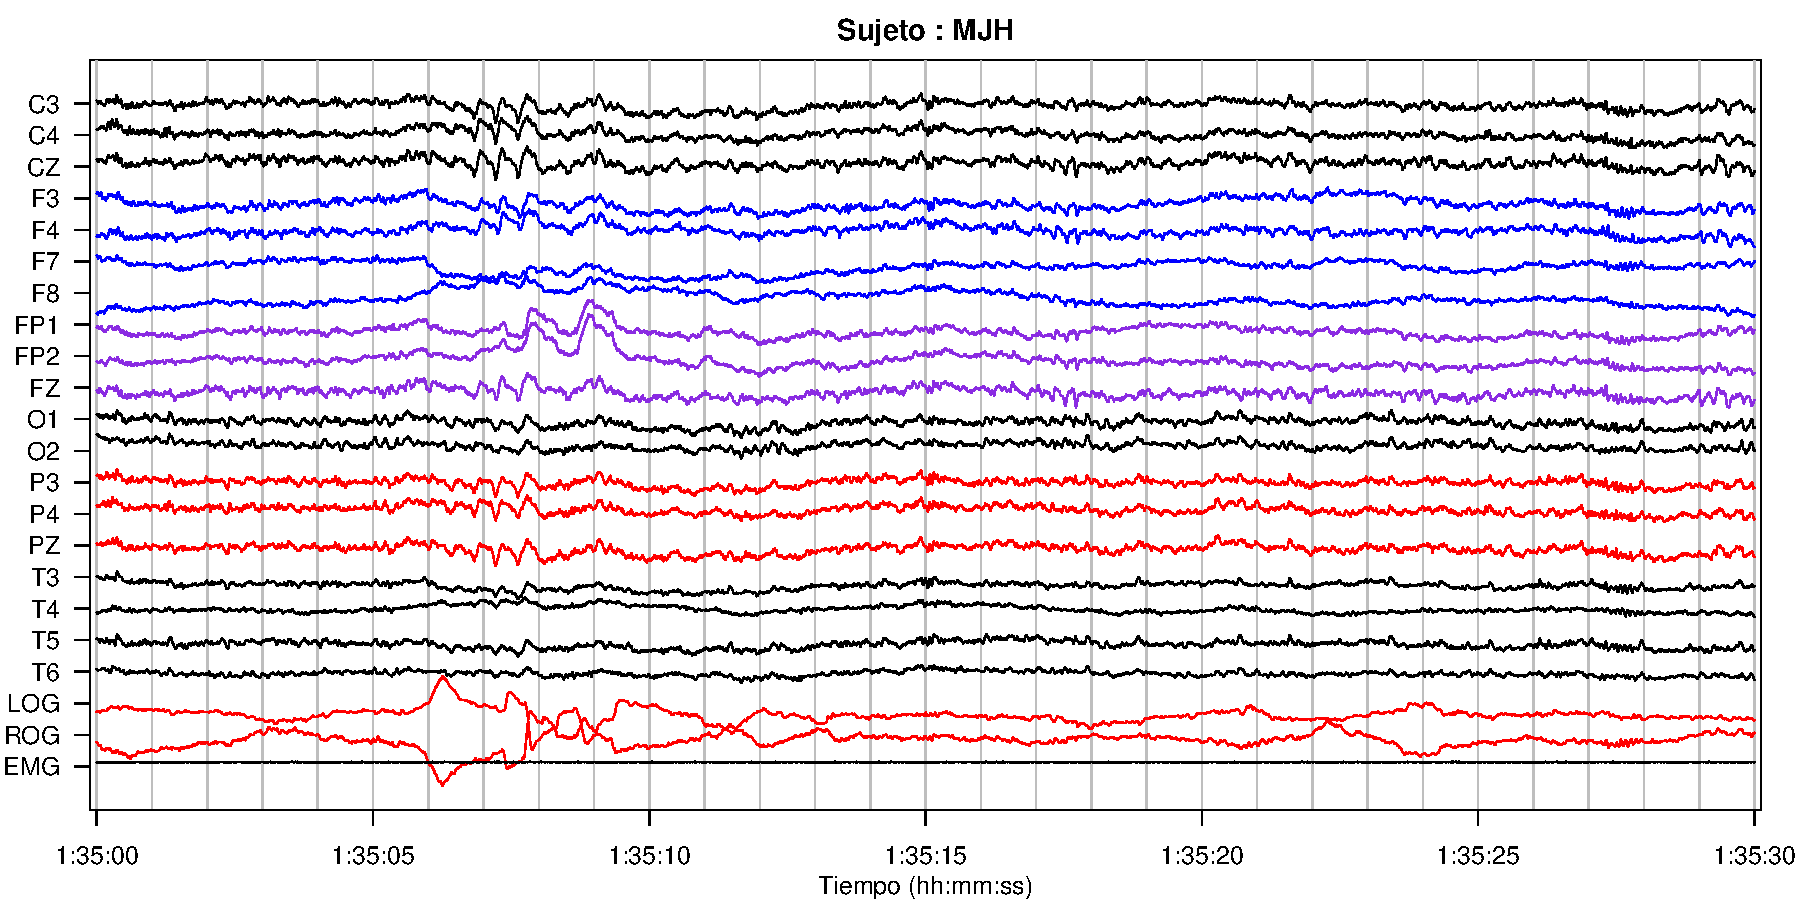
\includegraphics[width=\linewidth]
{./img_ejemplos/MJH_190_PDG_lucirse_PSG.pdf}
\caption{Registro de PSG en el sujeto MJH durante sue\~no MOR. N\'otese que el canal EMG permanece 
silente (indicativo de aton\'ia muscular) mientras que los canales ROG y LOG exhiben actividad de 
gran amplitud y sincronizaci\'on (movimientos oculares r\'apidos), caracter\'isticas indicativas de
la etapa de sue\~no.}
\label{ejemplos_mor}
\end{figure}

%textwidth: \printinunitsof{cm}\prntlen{\textwidth}
%
%linewidth: \printinunitsof{cm}\prntlen{\linewidth}

%%%%%%%%%%%%%%%%%%%%%%%%%%%%%%%%%%%%%%%%%%%%%%%%%%%%%%%%%%%%%%%%%%%%%%%%%%%%%%%%%%%%%%%%%%%%%%%%%%%
%%%%%%%%%%%%%%%%%%%%%%%%%%%%%%%%%%%%%%%%%%%%%%%%%%%%%%%%%%%%%%%%%%%%%%%%%%%%%%%%%%%%%%%%%%%%%%%%%%%
%%%%%%%%%%%%%%%%%%%%%%%%%%%%%%%%%%%%%%%%%%%%%%%%%%%%%%%%%%%%%%%%%%%%%%%%%%%%%%%%%%%%%%%%%%%%%%%%%%%
%%%%%%%%%%%%%%%%%%%%%%%%%%%%%%%%%%%%%%%%%%%%%%%%%%%%%%%%%%%%%%%%%%%%%%%%%%%%%%%%%%%%%%%%%%%%%%%%%%%


%\input{./texto/matematicas.tex}
%%%%%%%%%%%%%%%%%%%%%%%%%%%%%%%%%%%%%%%%%%%%%%%%%%%%%%%%%%%%%%%%%%%%%%%%%%%%%%%%%%%%%%%%%%%%%%%%%%%
%%%%%%%%%%%%%%%%%%%%%%%%%%%%%%%%%%%%%%%%%%%%%%%%%%%%%%%%%%%%%%%%%%%%%%%%%%%%%%%%%%%%%%%%%%%%%%%%%%%
%%%%%%%%%%%%%%%%%%%%%%%%%%%%%%%%%%%%%%%%%%%%%%%%%%%%%%%%%%%%%%%%%%%%%%%%%%%%%%%%%%%%%%%%%%%%%%%%%%%
%%%%%%%%%%%%%%%%%%%%%%%%%%%%%%%%%%%%%%%%%%%%%%%%%%%%%%%%%%%%%%%%%%%%%%%%%%%%%%%%%%%%%%%%%%%%%%%%%%%

\section{Matemáticas}

%
%El cuerpo central de este trabajo es averiguar sin este modelo de tipo estocástico para los datos
%permite la hipótesis de que los procesos estocásticos involucrados son estacionarios, cuando menos en
%un sentido débil.

Existe una larga tradición en las ciencias biomédicas para entender (y modelar) las señales
electrofisiológicas en términos de ondas y frecuencias, en parte debido a que fundamentalmente son
fenómenos eléctricos \cite{Kaiser00}.
El enfoque que se aborda, a \textit{grosso modo}, es asociar la \textit{energía} de una señal con 
la norma inducida por un producto interno, luego usar una base de un espacio (\textit{componentes 
de frecuencia}) para estudiar cómo se reparte esta energía entre tales elementos;
en concreto,
esto se logrará usando una generalización de la base Fourier para la familia de 
procesos estocásticos \textit{semi-estacionarios}.

Cabe mencionar que se propone como hipótesis que las señales constituyen un fenómeno 
predominantemente estocástico; esto no significa que las señales sean completamente aleatorias, sino 
que el posible no-determinismo está considerado en el modelo.
Por otro lado, aunque las señales sólo son registrables en un conjunto finito de puntos en el 
tiempo, se supone que el fenómeno ocurre efectivamente \textit{a tiempo continuo}, lo cual 
permitirá asumir algunas propiedades para el modelo.

Una vez formulado el modelo descrito, el objetivo principal es estudiar si éste es adecuado (en un 
sentido estadístico) para las señales que conforman el polisomnograma, o si pueden se explicadas
mejor como procesos estocásticos débilmente estacionarios (un modelo más particular). Dado el 
enfoque descrito, la comparación entre modelos se hará \textit{en términos ondas y frecuencias}.

%%%%%%%%%%%%%%%%%%%%%%%%%%%%%%%%%%%%%%%%%%%%%%%%%%%%%%%%%%%%%%%%%%%%%%%%%%%%%%%%%%%%%%%%%%%%%%%%%%%

\subsection{Transformada de Fourier}

La exposición inicia con los espacios de las \textbf{series $\boldsymbol{p}$-sumables}
($\lp$), y las  \textbf{funciones $\boldsymbol{p}$-integrables} sobre un intervalo 
$I \subseteq \R$ ($\llp$).
%; en el presente trabajo sólo se usarán los casos $p=1,2$.
%
%\begin{align}
%\ell^{p} &:= \left\{ s: \Z\rightarrow\C \talque \sum_{n=-\infty}^{\infty} \abso{s(n)}^{p} < \infty \right\}
%\label{lpdef} \\
%L^{p}[I] &:= \left\{ S: I\rightarrow\C \talque \int_I \abso{S(t)}^{p} dt < \infty \right\}
%\label{llpdef}
%\end{align}
\begin{align*}
\ell^{p} &:= \left\{ s: \Z\rightarrow\C \talque \sum_{n=-\infty}^{\infty} \abso{s(n)}^{p} < \infty \right\}
\\
L^{p}[I] &:= \left\{ S: I\rightarrow\C \talque \int_I \abso{S(t)}^{p} dt < \infty \right\}
\end{align*}

Estos espacios admiten las operaciones $+$, $\cdot$ y multiplicación por escalares complejos de la 
manera usual.%, es decir

%\begin{align*}
%s, z \in \lp, c \in \C \Rightarrow 
%[s+z](n) &= s(n) + z(n) \\
%[s\cdot z](n) &= s(n) z(n) \\
%[c \cdot s](n) &= s(n)c \\
%S, Z \in \llp, c \in \C \Rightarrow 
%[S+Z](t) &= S(t) + Z(t) \\
%[S\cdot Z](t) &= S(t)  Z(t) \\
%[c \cdot S](t) &= S(t)c
%\end{align*}
%
%En las próximas líneas se seguirán usando $s, z, S, Z, c$.

Para el caso particular $p=2$, los conjuntos $\ldos$ y $\lldos$ admiten los siguientes productos 
internos:
%
\begin{align*}
\left\langle s,z \right\rangle &= \sum_{n=-\infty}^{\infty} s(n) \overline{z(n)}\\
\left\langle S,Z \right\rangle &= \int_I S(t) \overline{Z(t)} dt
\end{align*}

Usando dichos productos internos, junto con las normas y métricas que inducen, los conjuntos 
$\ldos$ y $\lldos$ tienen estructura de \textbf{espacio de Hilbert}.

Con las definiciones anteriores, que muestran que $\ldos$ y $\lldos$ son \textit{muy}
parecidos, se puede formular unas definición para la transformada de Fourier como una equivalencia
entre estos espacios.

%{De manera pragm\'atica, en el presente trabajo la 
%palabra  'frecuencia' se usar\'a para referirse a la cantidad $q$ en expresiones del tipo 
%$e^{i q t}$}

\begin{definicion}[Serie de Fourier]
Sea $S: \R \rightarrow \C$ una función periódica con periodo $2T$ y tal que 
$S \in L^{2}\left[[-T,T]\right]$. Se dice que $A$ es la serie de Fourier para $S$ si cumple que
\begin{equation*}
A(n) = \frac{1}{2 T} \simint{T} S(t) e^{-\nicefrac{ i \abso{n} t}{2T}} dt
\end{equation*}
%Adicionalmente, la función $\mathcal{F} : \lldos \rightarrow \ldos : S \mapsto A$  recibe el nombre
%de \textbf{Transformada de Fourier}
\label{FourierClasico}
\end{definicion}

\begin{definicion}[Transformada de Fourier]
Sean $S$ y $A$ como en la definición \ref{FourierClasico}. Se le llama transformada de Fourier a la
función $\mathcal{F}_T : L^{2}\left[[-T,T]\right] \rightarrow \ldos : S \mapsto A$
\end{definicion}

Puede interpretarse a $A$ como las \textit{coordenadas} de $S$ en $L^{2}\left[[-T,T]\right]$, 
usando una base de funciones $\left\{ e^{\nicefrac{i \abso{n} t}{2 T}} \right\}_{n\in \Z}$, las
cuales resultan ser ortonormales; esta base en particular es conocida como la \textbf{base de 
Fourier}.
Se demuestra en el anexo A que $\mathcal{F_T}$ está bien definida en el sentido de 
tener efectivamente el dominio y codominio indicados. Así mismo, cabe mencionar las siguientes 
propiedades de $\mathcal{F}_T$
\begin{itemize}
\item Es lineal, es decir, $\mathcal{F}_T[cS + Z] = c\mathcal{F}_T[S] + \mathcal{F}_T[Z]$

\item \textbf{No} es invertible, aunque se le suele definir una
pseudoinversa\footnote{$\mathcal{F}_T^{\text{inv}}$ es \textit{exacta} salvo por la suma
de alguna función $S_0$ tal que $\int_{-T}^{T}\abso{S_0(t)}dt = 0$} como
\begin{equation*}
\mathcal{F}_{T}^{\text{inv}} : \ldos \rightarrow L^{2}\left[[-T,T]\right] :
A \mapsto \sum_{n -\infty}^{\infty} A(n) e^{\nicefrac{i \abso{n} t}{2 T}}
\end{equation*}
\end{itemize}

Con esta terminología se define, de manera pragmática, la \textbf{energía disipada} y la 
\textbf{potencia} de una función $S$ en un intervalo $[a,b]$ como 
\begin{align*}
\text{energía}[S]_{[a,b]} &= \int_a^{b} \abso{S(t)}^{2} dt \\
\text{potencia}[S]_{[a,b]} &= \frac{1}{b-a} \int_a^{b} \abso{S(t)}^{2} dt
\end{align*}
%
%Estas últimas definiciones cobran importancia a la luz del teorema \ref{parseval}: la energía de 
%una función equivale a su norma.

Una consecuencia interesante de este concepto de energía frente al teorema \ref{parseval} es que la 
energía disipada por una función equivale a la suma de la energía disipada por sus 
\textit{componentes} en la base de Fourier.
Conviene, entonces, definir una función que \textit{desglose} estos \textit{aportes}.

\begin{teorema}[Parseval]
Sea $S \in L^{2}\left[[-T,T]\right]$, y sea $A = \mathcal{F}[S]$. Se cumple que
\begin{equation*}
\int_{-T}^{T} \abso{S(t)}^{2} dt = \sum_{n=-\infty}^{\infty} \abso{A(n)}^{2}
\end{equation*}
\label{parseval}
\end{teorema}

\begin{definicion}[Espectro de potencias]
Sea $S \in L^{2}\left[[-T,T]\right]$, y sea $A = \mathcal{F}[S]$. Se llama espectro de potencias 
para $S$ a la función $h_S : \R \rightarrow \R $, definida como
\begin{equation*}
h_S(\omega) = 
\begin{cases}
\abso{A(n)}^{2} & \text{ , si } \omega = \nicefrac{n}{2T}, \text{   con } n\in \mathbb{Z} \\
0 & \text{ ,  otro caso}
\end{cases}
\end{equation*}
\label{espec}
\end{definicion}

Un elemento que será de crucial importancia en el desarrollo posterior es la \textbf{convolución}, 
$\ast$, una tercera operación binaria definida en estos espacios como
%
\begin{align*}
[s \ast z] (\tau) &= \sum_{n=-\infty}^{\infty} s(n) \overline{z(\tau-n)} \\
[S \ast Z] (\tau) &= \int_I S(t) \overline{Z(\tau-t)}
\end{align*}
%
donde $\overline{c}$ es el conjugado complejo de $c$. 
%La convolución es conmutativa y asociativa con la suma. 
Esta operación cobra importancia por la forma en que se relaciona con $\mathcal{F}_T$
%
\begin{teorema}%[de la convolución]
Sean $S,Z \in L^{2}\left[[-T,T]\right]$, entonces se satisface que
\begin{align*}
\mathcal{F}_T[S\ast Z]  &= \mathcal{F}_T[S] \cdot \mathcal{F}_T[Z] \\
\mathcal{F}_T[S\cdot Z] &= \mathcal{F}_T[S] \ast  \mathcal{F}_T[Z] \\
\end{align*}
\label{t_convolucion}
\end{teorema}

\subsubsection{Generalizaciones}

La primera gran generalización sobre la transformada de Fourier es para el conjunto de funciones 
$L^{1}\left[ \R \right]$, definido como en la sección anterior; éste también es un espacio de 
Hilbert usando el producto interno descrito.
La generalización propuesta, teorema \ref{intFourier}, sólo se diferencia en que no se exige que 
la función sea periódica y en el espacio que actúa; 
es quizá más llamativo el que el codominio de $\mathcal{F}_\infty$ no sea $\ldos$ sino $\lldos$,
%es decir que su codominio no son series sino funciones integrables
lo cual afecta cómo deben interpretarse los \textit{componentes de frecuencia generalizados}. La 
discusión pertinente se efectúa en el anexo B.

\begin{definicion}[Integral de Fourier]
Sea $S \in L^{1}\left[\R\right]$. Se dice que $A$ es la integral de Fourier para $S$ si cumple que
\begin{equation*}
A(\omega) = \intR S(t) e^{- i \omega t} dt
\end{equation*}
%Adicionalmente, la función $\mathcal{F} : \lldos \rightarrow \ldos : S \mapsto A$  recibe el nombre
%de \textbf{Transformada de Fourier}
\label{intFourier}
\end{definicion}

\begin{definicion}[Transformada de Fourier]
Sean $S$ y $A$ como en la definición \ref{intFourier}. Se le llama transformada de Fourier a la
función $\mathcal{F}_\infty : L^{1}\left[\R\right] \rightarrow \ldos : S \mapsto A$
\end{definicion}

Una forma de \textit{relacionar} a los $\mathcal{F}_T$ con $\mathcal{F}_\infty$ es tomar una
función $S \in L^{1}\left[\R\right]$ y para cada $T$ definir una continuación periódica de $S$
%, $S_T$
%\begin{equation*}
\begin{center}
$\displaystyle S_T(t) = S(t_0) $, 
%\end{equation*}
con $\displaystyle -T\leq t_0 \leq T$ y $\displaystyle \frac{t-t_0}{2T} \in \Z$
\end{center} 
%
Posteriormente puede hacerse que
%\begin{equation*}
$\lim_{T\rightarrow \infty} \mathcal{F}_T[S_T] = \mathcal{F}_{\infty}$.
%\end{equation*}
%Este proceso suele interpretarse como que $\mathcal{F}_\infty$ es una versión de la transformada
%de Fourier donde se permite que la función sea periódica con periodo infinito,
%%el periodo de la función ($\nicefrac{1}{\text{frecuencia}}$) sea
%%infinitamente grande, 
%o que la distancia entre frecuancias sea infinitamente pequeño.
%
Dado que las funciones definidas en \ref{FourierClasico} y en \ref{intFourier} serán importantes 
en lo que prosigue, conviene introducir una segunda generalización que abarque a ambas, para lo que
se acude al concepto de integrales en el sentido de Lebesgue-Stieltjes (en un anexo)

\begin{definicion}[Integral de Fourier-Stieltjes]
Sea $S: \R\rightarrow \C$. Se dice que $F$ es la integral de Fourier-Stieltjes para $S$ si ésta 
puede escribirse como
\begin{equation*}
S(x) = \intR e^{- i \omega t} dF(\omega)
\end{equation*}
donde la integral está definida en el sentido de Lebesgue-Stieltjes, y la igualdad se cumple
casi en todas partes
%Adicionalmente, la función $\mathcal{F} : \lldos \rightarrow \ldos : S \mapsto A$  recibe el nombre
%de \textbf{Transformada de Fourier}
\label{intFourierStieltjes}
\end{definicion}

%%%%%%%%%%%%%%%%%%%%%%%%%%%%%%%%%%%%%%%%%%%%%%%%%%%%%%%%%%%%%%%%%%%%%%%%%%%%%%%%%%%%%%%%%%%%%%%%%%%

\subsection{Estacionariedad débil}

\begin{definicion}[Proceso estoc\'astico]
Un proceso estocástico \xt es una familia de variables aleatorias reales, 
indexadas por $t \in T$.
\label{proc_estocastico}
\end{definicion}

Respecto al conjunto $T$ que indexa a un proceso estocástico, y que será referido como 
\textit{tiempo}, conviene introducir dos grandes grupos para los mismos
\begin{itemize}
\item \textit{Continuo} si $T$ es un intervalo cerrado
\item \textit{Discreto} si $T$ es de la forma 
$\{ t_0 + n \delta \lvert n \in U \subseteq \mathbb{Z} \}$
\end{itemize}

Los procesos a tiempo discreto contemplan conjuntos finitos e infinitos de puntos en el tiempo.
No se manejan discutirá sobre otros tipos de tiempo en este trabajo.

Como notación, se usará \xt  para el proceso estocástico y $X(t)$ para una de las variables
aleatorias que lo componen; de la misma manera $x(t)$ es una realización de $X(t)$ y $F_{X(t)}$ 
es la función de probabilidad acumulada para $X(t)$.

\begin{definicion}[Estacionariedad débil]
Un proceso estocástico \xt es débilmente estacionario si y sólo si para cualesquiera tiempos 
admisibles\footnote{El término \textit{tiempos admisibles} significa que la definición es la misma
para diferentes tipos de tiempo, bajo las restricciones pertinente} $t$, $s$ se tiene que
\begin{itemize}
\item $\E{X(t)} = \mu_X$
\item $\Var{X(t)} = \sigma^{2}_X$
\item $\Cov{X(t),X(s)} = \rho_X (s-t)$
\end{itemize}
Donde $\mu_X$, $\sigma^{2}_X$ son constantes, $\rho_X(\tau)$ es una función que únicamente 
depende de $\tau$
\label{est_orden_primera}
\end{definicion}

Adicionalmente se supondrá que las señales en el electroencefalograma (EEG) son continuas, cuando menos
el sentido de media cuadrática

\begin{definicion}[Continuidad estocástica en media cuadrática]
Un proceso estocástico a tiempo continuo $\{ X(t) \}$ es estocásticamente continuo, en el 
sentido de media cuadrática, en un tiempo admisible $t_0$ si y sólo si
\begin{equation*}
\lim_{t \rightarrow t_0} \E{\left( X(t) - X(t_0) \right)^{2}} = 0
\end{equation*}
\label{cont_est}
\end{definicion}

\subsubsection{Función de densidad espectral}

\begin{definicion}[Función de densidad espectral (FDE)]
Sea $\{X(t)\}$ un proceso estocástico en tiempo continuo, débilmente estacionario. Se define la 
función de densidad espectral (FDE) para $\{X(t)\}$ como
%\begin{equation*}
%h(\omega) = \lim_{T\rightarrow \infty} \E{ \frac{ \left| G_T(\omega) \right|^{2}}{2 T} }
%\end{equation*}
\begin{equation*}
h(\omega) = \lim_{T\rightarrow \infty} \E{ \frac{1}{2T} \frac{1}{2 \pi}
\abso{ \int_{-T}^{T} X(t) e^{-i \omega t} dt}^{2} }
\end{equation*}
%Donde $G_T (\omega) = \frac{1}{\sqrt{2 \pi}} \int_{-T}^{T} X(t) e^{-i \omega t} dt$
\label{FDE}
\end{definicion}

\begin{definicion}[Función de espectro integrado]
Sea $\{X(t)\}$ un proceso estoc\'astico a tiempo continuo, débilmente estacionario. Se define la 
función de espectro integrado para $\{X(t)\}$ como
\begin{equation*}
H(\omega) = \int_{-\infty}^{\omega} h(\lambda) d\lambda
\end{equation*}
Donde $h$ es la función de densidad espectral para $\{X(t)\}$
\label{FDE_integrado}
\end{definicion}

Si la FDE, $h$, est\'a bien definida en todos sus puntos, entonces la función de espectro 
integrado ($H$) satisface que $H\prima= h$ y se dirá que el proceso tiene un \textbf{espectro 
puramente continuo}; si $H$ tiene una forma escalonada, con escalones rectos, se dirá que es un 
\textbf{espectro puramente discreto}.
Como es de esperarse, cada tipo de proceso tiene característica diferentes y se puede estudiar 
mejor con herramientas diferentes; para el caso de procesos con un espectro mixto (ninguno de los 
anteriores), se exhiben herramientas que los reducen a estos casos 'puros'.

Cabe destacar que, por como se definió la FDE integrada, ésta es una función positiva, 
no-decreciente, y que en $-\infty$ vale 0; esta observación será importante.

\begin{teorema}[Wiener-Khinchin]
Una condición suficiente y necesaria para que $\rho$ sea una función de autocorrelación de 
algún proceso estocástico a tiempo continuo $\{X(t)\}$ débilmente estacionario y 
estocásticamente continuo, es que exista una función $F$ que tenga las siguientes propiedades
\begin{itemize}
\item Monótonamente creciente
\item $F(-\infty) = 0$
\item $F(+\infty) = 1$
\end{itemize}
y tal que para todo $\tau \in \R$ se cumple que
\begin{equation*}
\rho(\tau) = \intR e^{i \omega \tau} dF(\omega)
\end{equation*}
\label{t_wienerkhinchin}
\end{teorema}

\begin{teorema}[Wold]
Una condición suficiente y necesaria para que $\rho$ sea una función de autocorrelación de 
algún proceso estocástico a tiempo discreto $\{X(t)\}$ débilmente estacionario es que exista 
una función $F$ con las siguientes propiedades
\begin{itemize}
\item Monótonamente creciente
\item $F(-\pi) = 0$
\item $F(+\pi) = 1$
\end{itemize}
y tal que para todo $\tau \in \R$ se cumple que
\begin{equation*}
\rho(\tau) = \intPI e^{i \omega \tau} dF(\omega)
\end{equation*}
\label{t_wold}
\end{teorema}

\subsection{Representación espectral}

\begin{teorema}
Sea $\{X(t)\}$ un proceso estocástico a tiempo continuo débilmente estacionario de media 0 y 
estocásticamente continuo en el sentido de media cuadrática. Entonces, existe un proceso 
ortogonal $\{Z(\omega)\}$ tal que, para todo tiempo $\omega$ admisible, se puede 
escribir\footnote{La integral se encuentra definida en el sentido de media cuadrática.}
\begin{equation*}
X(t) = \intR e^{i t \omega} dZ(\omega)
\end{equation*}
Donde el proceso $\{Z(t)\}$ tiene las siguientes propiedades para todo $\omega$
\begin{itemize}
\item $\E{dZ(\omega)} = 0$
\item $\E{\abso{dZ(\omega)}^{2}} = dH(\omega)$
\item $\Cov{dZ(\omega),dZ(\lambda)} = 0 \Leftrightarrow \omega \neq \lambda$
\end{itemize}
Donde $dH(\omega)$ la FDE integrada de $\{X(t)\}$
\label{rep_espectral}
\end{teorema}

En virtud del teorema de Wold, se puede tener una variante del teorema \ref{rep_espectral}
para procesos a tiempo discreto, razón por la cual  
tal representación es referida como \textbf{representación de Wold-Cramér}.

%%%%%%%%%%%%%%%%%%%%%%%%%%%%%%%%%%%%%%%%%%%%%%%%%%%%%%%%%%%%%%%%%%%%%%%%%%%%%%%%%%%%%%%%%%%%%%%%%%%

\subsection{Estimación}

Conviene introducir estimadores para la función de autocovarianza de un proceso débilmente 
estacionario, $\{ X(t) \}$, a partir de un conjunto de $N$ observaciones equiespaciadas en el 
tiempo con separación $\Delta t$; se denotará a estas observaciones como 
$x_1, x_2 , \dots, x_N$. Como se cumple la siguiente propiedad para la función de autocovarianza, 
$R$, por definición
\begin{equation*}
R(\tau) = \E{X(n\Delta t)X(n\Delta t + \tau)} \text{  ,  } n = 0, 1, 2,  3,\dots, N
\end{equation*}
el estimados estándar para $R$ está dado por la siguiente expresión
\begin{equation*}
\widehat{R}(\tau) = \frac{1}{N-\abso{\tau}} 
\sum_{t = 1}^{N-\abso{\tau}} x_t x_{t+\abso{\tau}}
\label{estimador_R}
\end{equation*}

Se puede demostrar que $\widehat{R}$ es un estimador insesgado\footnote{Un estimador para el 
parámetro $\theta$, $\widehat{\theta}$, se dice \textbf{insesgado} si 
$\E{\widehat{\theta}}=\theta$} y consistente\footnote{Un estimador para el parámetro $\theta$ que 
depende de $N$ observaciones, 
$\widehat{\theta}_N$, se dice \textbf{consistente} si 
$\lim_{N\rightarrow \infty} \Var{\widehat{\theta}_N} = 0$} 
para $R$; sin embargo conviene introducir un estimador diferente para $R$
\begin{equation*}
\aste{R}(\tau) = \frac{1}{N} 
\sum_{t = 1}^{N-\abso{\tau}} x_t x_{t+\abso{\tau}}
\label{estimador_R_ast}
\end{equation*}

\begin{teorema}
Sean $x_1, x_2 , \dots, x_N$ observaciones de un proceso estocástico de media cero y varianza
finita. Se puede calcular el periodograma para estos datos como
\begin{equation*}
I_N(\omega) = 2 \sum_{r = -(N-1)}^{N-1} \aste{R}(r) \COS{r \omega}
\end{equation*}
Donde $\aste{R}$ es el estimador para la función de autocovarianza del proceso, calculado como
$\widehat{R}(\tau) = \frac{1}{N-\abso{\tau}} \sum_{t = 1}^{N-\abso{\tau}} x_t x_{t+\abso{\tau}}$
\label{periodograma_rho}
\end{teorema}

Se puede demostrar que el periodograma es un estimador insesgado de la FDE para los proceso 
considerados; sin embargo, si el proceso tuviera un espectro puramente continuo, ocurre que 
$\lim_{N\rightarrow \infty} \Var{I_N(\omega)} = h^{2}(\omega)$, con $h$ la FDE del proceso: el 
periodograma, en general, no es consistente.
En parte esto ocurre porque el periodograma depende de los estimadores para la función de 
autocovarianza, $\est{R}$, evaluada en todos los puntos posibles: para calcular $\est{R}$ en 
valores muy altos se requieren puntos muy alejados, los cuales son menos abundantes e implican 
una mayor varianza.

Si efectivamente el periodograma aumenta su varianza cuando incluye las 'colas' de la función de 
autocovarianza, entonces una solución es evitarlas, multiplicando por una función de pesos. 
Tales consideraciones dan origen a estimadores de la forma
\begin{equation*}
\est{h}(\omega) = \frac{1}{2\pi} \sum_{s = -(N-1)}^{N-1} 
\lambda(s) \aste{R}(s) e^{i \omega t}
\label{ventaneando}
\end{equation*}
donde la función de pesos, $\lambda$, es referida como \textbf{ventana de retrasos}. Para 
estudiar las propiedades estos estimadores, conviene reescribirlos en función del periodograma

\begin{equation*}
\est{h}(\omega) = \intPI I_N(\theta) W(\omega-\theta) d\theta
\end{equation*}
donde $W$ es la transformada de Fourier finita de $\lambda$
\begin{equation*}
W(\theta) = \frac{1}{2\pi} \sum_{s = -(N-1)}^{N-1} \lambda(s) e^{-is\theta}
\end{equation*}

Cabe destacar la forma que adopta $\est{h}$ como la convolución $I_N \ast W$, que bien puede 
entenderse como que $W$ es una función de pesos en el 'dominio de las frecuencias'; por ello, $W$ 
es referida como \textbf{ventana de retrasos}.
En la tabla \ref{ventanas} hay una lista corta de algunas funciones tipo ventana. Estos estimadores 
son consistentes y sesgados, aunque son asintóticamente insesgados.

%%%%%%%%%%%%%%%%%%%%%%%%%%%%%%%%%%%%%%%%%%%%%%%%%%%%%%%%%%%%%%%%%%%%%%%%%%%%%%%%%%%%%%%%%%%%%%%%%%%

\begin{proposicion}
Sean $u$ y $v$ dos funciones tipo \textit{pseudo $\delta$ de Dirac}, es decir, unimodales con un
máximo  y (...). Si $u$ tiene una concentración muy alta, con relación a $v$, entonces
\begin{equation*}
\intR u(x) v(x+k) dx \approx v(k) \intR u(x) dx
\end{equation*}
\label{pseudo_d}
\end{proposicion}

%%%%%%%%%%%%%%%%%%%%%%%%%%%%%%%%%%%%%%%%%%%%%%%%%%%%%%%%%%%%%%%%%%%%%%%%%%%%%%%%%%%%%%%%%%%%%%%%%%%

\subsection{Estimador de doble ventana}

Respecto a la estimación del espectro local se usa el \textbf{estimador de doble ventana}, 
técnica introducida por Priestley \cite{Priestley69} y que requiere dos funciones, $w_\tau$ y 
$g$, que funcionan como ventana de retrasos y como filtro lineal, respectivamente.
%
En cuando a $g$, se define a $\Gamma(u) = \intR g(u) e^{i u \omega} du$ y se les pide que
\begin{equation*}
2\pi \int_{-\infty}^{\infty} \lvert g(u) \lvert^{2} du 
= 
\int_{-\infty}^{\infty} \lvert \Gamma(\omega) \lvert^{2} d\omega
= 1
\end{equation*}

Cabe mencionar que las ventanas espectrales mostradas en la tabla \ref{ventanas} bien 
pueden cumplir las propiedades requeridas para ser filtros.
Posteriormente se define el estimador $U$ con el objetivo de asignar pesos en el tiempo para estimar
a la FDE
% en el tiempo dado; más aún, $U$ sirve 
%como una aproximación de la representación de Wold-Cramér para 
%el proceso.
\begin{equation*}
U(t,\omega) = \int_{t-T}^{t} g(u) X({t-u}) e^{i \omega (t-u)} du
\end{equation*}

Bajo el entendido que la función $\Gamma$ converge a una función tipo \dirac, puede 
considerarse que 
$\E{\abso{U(t,\omega)}^{2}} \approx f_t(\omega)$; sin embargo, se demuestra en \cite{Priestley66} 
que $\Var{\abso{U(t,\omega)}^{2}} \nrightarrow 0$.
%
Debido a ello se usa una segunda función tipo ventana,
%, para 'suavizar' el estimador y hacerlo consistente (
de forma similar al periodograma.
Se considera la función $W_\tau$, ventana de retrasos, y su respectiva ventana espectral 
$w_\tau$; deben satisfacer las siguientes propiedades:
\begin{itemize}
\item $w_{\tau}(t) \geq 0$ para cualesquiera $t$, $\tau$
\item $w_{\tau}(t) \rightarrow 0$ cuando $\lvert t \lvert \rightarrow \infty$, para todo $\tau$
\item $\displaystyle \int_{-\infty}^{\infty} w_{\tau}(t) dt = 1$ para todo $\tau$
\item $\displaystyle \int_{-\infty}^{\infty} \left( w_{\tau}(t) \right)^{2} dt < \infty$ para todo $\tau$
\item $\exists C$ tal que  
$\displaystyle \lim_{\tau\rightarrow\infty} \tau \int_{-\infty}^{t} \abso{ W_{\tau}(\lambda) }^{2} d\lambda = C$
\end{itemize}

%Por ejemplo, la ventana de Daniell satisface estas propiedades; para ello, conviene calcular que
%$\lim_{\tau\rightarrow\infty} \tau \int_{t-T}^{t} \lvert W_{\tau}(\lambda) \lvert^{2} d\lambda = 2\pi$;
%más aún, 
Cabe mencionar que todas las ventanas mostradas en \ref{ventanas} satisfacen las propiedades 
anteriores.
Finalmente, se define el estimador $\est{f}$ para las FDE normalizada, $f_t$, como
\begin{equation*}
\widehat{f}(t,\omega) = \int_{t-T}^{t} w_{T'}(u) \lvert U(t-u,\omega) \lvert^{2} du
\label{estimador_doble_ventana}
\end{equation*}

Fue demostrado por Priestley \cite{Priestley65} que los estimadores de doble ventana son 
asintóticamente insesgados y consistentes, y propone las siguientes aproximaciones:
%conviene exhibir las siguientes expresiones aproximadas propuestas en aquél trabajo
\begin{itemize}
\item $\displaystyle
\E{\est{f}(t,\omega)} \approx 
\intR \widetilde{f}(t,\omega+\theta) \abso{\Gamma(\theta)}^{2} d\theta$
\item $\displaystyle
\Var{\est{f}(t,\omega)} \approx \frac{C}{\tau} \left( \overline{f}^{2}(\omega) \right)
\intR \abso{\Gamma(\theta)}^{4} d\theta $
\end{itemize}

donde las funciones $\widetilde{f}$ y $\overline{f}$ son versiones 'suavizadas' de la FDE 
normalizada, $f$, y están definidas de la siguiente manera
\begin{equation*}
\widetilde{f}(t,\omega+\theta) = 
\intR W_{\tau}(u) f(t-u,\omega+\theta) du
\end{equation*}
\begin{equation*}
\overline{f}^{2} (t,\omega) =
\frac{\intR f^{2}\left(t-u,W_{\tau}^{2}(u)\right) du}
{\intR \left( W_{\tau}(u) \right)^{2} du}
\end{equation*}

Como $W_{\tau}$ funciona como ventana espectral, converge a una 
función tipo \dirac; luego $\widetilde{f}$ es aproximadamente la convolución 
$\widetilde{f}(t,\omega+\theta) \approx \delta_t \ast f(\bullet,\omega+\theta)$. 
Una aproximación muy similar 
puede hacerse respecto al segundo término, de modo que $\widetilde{f}\approx f$ y 
$\overline{f}^{2}\approx f^{2}$.
Tales aproximaciones serán mejores en tanto las ventanas $w_{\tau}$ y $W_{\tau}$ sean más 
cercanas a funciones tipo \dirac.
%; más aún, una condición adecuada es que estas funciones 
%tengan una forma 'más delgada' que el espacio entre los tiempos y frecuencias donde se estimará 
%$f$.
Dicho esto, se pueden hacer las siguientes aproximaciones, un poco más arriesgadas:
\begin{itemize}
\item $\displaystyle \E{\est{f}(t,\omega)} \approx f(t,\omega)$
\item $\displaystyle \Var{\est{f}(t,\omega)} \approx 
\frac{C}{\tau} f^{2}(t,\omega) \intR \abso{\Gamma (\theta)}^{4} d\theta$
\end{itemize}

\subsection{Prueba de Priestley-Subba Rao}

Una propiedad interesante de poder estimar el espectro evolutivo de un proceso, a partir de una 
realización del mismo, es la capacidad para identificar si éste pudiera reducirse al espectro 
usual, definido para procesos débilmente estacionarios --bastaría con revisar si el espectro 
estimado es constante en el tiempo.
%En otras palabras, el espectro evolutivo puede usarse como herramienta para decidir si un proceso 
%es estacionario.

La prueba de estacionariedad propuesta por Priestley y Subba Rao en 1969 \cite{Priestley69} tiene 
como \textit{ingrediente principal} un estimador muy particular para una cantidad que depende del 
espectro, con propiedades estadísticas adecuadas para detectar la posible estacionariedad.

Sea \xt que se tiene un proceso semi-estacionario y sea \xtd un conjunto de observaciones del 
proceso, espaciadas uniformemente en el tiempo.
Se construye a $\widehat{f}$, el estimador de doble ventana definido como en la sección anterior,
usando las funciones ventana $g_h$ y $w_\tau$, y sus respectivas transformadas de Fourier 
$\Gamma_h$ y $W_\tau$. Como se mencionó previamente, bajo las condiciones descritas se cumple que 
$\widehat{f}$ es un estimador consistente y aproximadamente insesgado para $f$, el espectro
evolutivo de \xt. Ahora bien, considerando las siguientes aproximaciones
%
\begin{itemize}
\item $\E{\widehat{f}(t,\omega)} \approx f(t,\omega)$
\item $\Var{\widehat{f}(t,\omega)} \approx 
\frac{C}{T} f^{2}(t,\omega) \intR \abso{\Gamma^{4}(\theta)} d\theta$
\end{itemize}
%
donde $C = \lim_{T\rightarrow \infty} T \intR \abso{W_T(\lambda)} d\lambda$.
Usando a $\widehat{f}$, se define el estimador $Y$ como el logaritmo de éste, 
$Y(t,\omega) = \log\left(\widehat{f}(t,\omega)\right)$, y que tiene las siguientes propiedades
%
\begin{itemize}
\item $\E{Y(t,\omega)} \approx \log\left(f(t,\omega)\right)$
\item $\Var{Y(t,\omega)} \approx 
\frac{C}{T} \intR \abso{\Gamma_h(\theta)}^{4} d\theta =: \sigma^{2}$
\end{itemize}
%

Cabe destacar que la varianza $Y$ no es formalmente independiente de $f$ sino que es 
\textit{aproximadamente independiente}, es decir, la varianza de $Y$ depende \textit{más} 
del propio estimador que del verdadero valor de $\log\circ f$.
Esto no es tan sorprendente tomando en cuenta el diseño del estimador de doble ventana, que otorga 
mayor importancia a la información local usando repetidamente la proposición \ref{pseudo_d}. Esta 
independencia asintótica sugiere que $Y$ puede verse como
%
%\begin{equation}
$Y(t,\omega) = \log\left(f(t,\omega) \right) + \varepsilon(t,\omega)$,
%\end{equation}
%
con $\E{\varepsilon(t,\omega)} \approx 0$ y $\Var{\varepsilon(t,\omega)} \approx \sigma^{2}$.

Más aún, es demostrado en \cite{Priestley66} que si $\abso{\omega-\omega_0}$ es suficientemente 
grande como para que 
$\intR \abso{\Gamma_h(\theta+\omega)}^{2}\abso{\Gamma_h(\theta+\omega_0)}^{2} d\theta \approx 0$,
entonces 
%
%\begin{itemize}
%\item 
$\Cov{Y(t,\omega),Y(t,\omega_0)} \approx 0$.
%\end{itemize}
%
Similarmente, si $\abso{t-t_0} >> \intR \abso{t} \abso{w_\tau (t)} dt $, entonces
%
%\begin{itemize}
%\item 
$\Cov{Y(t,\omega),Y(t_0,\omega)} \approx 0$.
%\end{itemize}

Bajo estas nuevas condiciones, es posible construir una versión discretizada de $Y$ tal que los 
componentes $\varepsilon$ sean estadísticamente independientes. Para ello se define una malla de 
puntos $(t_i,\omega_j)$, con $i = 1,\dots,I$ y  $j=1,\dots,J$, y posteriormente a la matriz $Y$ 
como $Y_{i,j} = Y(t_i,\omega_j)$, que satisface
%
\begin{itemize}
\item $Y_{i,j} = \log\left(f(t_i,\omega_j)\right) + \varepsilon_{i,j}$
\item $\E{\varepsilon_{i,j}} \approx 0$
\item $\Var{\varepsilon_{i,j}} \approx \sigma^{2} = 
\frac{C}{T} \intR \abso{\Gamma_h(\theta)}^{4} d\theta$
\item $\Cov{\varepsilon_{i,j},\varepsilon_{i_0,j_0}} \approx 0$ siempre que $(i,j)\neq (i_0,j_0)$
\end{itemize}

Ha sido sugerido por Jenkins [??] que si el número de puntos es suficientemente grande, entonces
las componentes de $Y$ siguen distribuciones aproximadamente normales, de modo que
$\varepsilon_{i,j} \sim N(0,\sigma^{2})$.

%\begin{figure}
%\centering
%\includegraphics[width=0.7\linewidth]{./img_diagramas/psr_simple.pdf}
%\caption{Representación diagramática de la implementación en R de la prueba PSR. Se omite 
%filtrado previo mediante el algoritmo STL (ver texto).}
%\label{diagrama_psr}
%\end{figure}

Habiendo definido al estimador $Y$ según de esta forma en su versión discretizada (proceso resumido
en el gráfico \ref{diagrama_psr}), es posible definir criterios estadísticos para determinar la 
estacionariedad débil usando a $Y$. El primer caso es definir, como hipótesis nula, un modelo 
general
%
\begin{equation*}
H_0 : \hspace{1em} Y_{i,j} = \mu + \alpha_i + \beta_j + \gamma_{i,j} + \varepsilon_{i,j}
\end{equation*}
%
donde $\varepsilon$ son como se definieron anteriormente. Respecto a los otros parámetros, $\mu$ 
representa el promedio de $Y$ (así $\alpha$, $\beta$, $\gamma$ tienen media cero), $\alpha$ y 
$\beta$ son las \textit{variaciones} de $Y$ en el tiempo y las frecuencias, respectivamente, y 
$\gamma$ abarca las \textit{variaciones} no-lineales; $\gamma$ y $\varepsilon$ se diferencían en 
que por diseño se sabe que $\varepsilon_{i,j} \sim N(0,\sigma^{2})$, mientras que no se ha supuesto 
nada sobre $\gamma$.

Para determinar la estacionariedad se define, como hipótesis alterna, un modelo el $Y$ es 
efectivamente constante en el tiempo
%
\begin{equation*}
H_A : \hspace{1em} Y_{i,j} = \mu + \alpha_i + \varepsilon_{i,j}
\end{equation*}
%
posteriormente se prueba si se puede rechazar $H_0$ a favor de $H_A$; para ello se evalúan los 
estadísticos de el cuadro \ref{cantidades_psr} y se verifican las hipótesis 
$\nicefrac{S_{I+R}}{\sigma^{2}} = 0$ (para $\gamma=0$)  y $\nicefrac{S_T}{\sigma^{2}} = 0$ (para 
$\beta=0$).
Por cómo se construyeron, estos estadísticos tienen distribuciones $\chi^{2}$, con los grados de 
libertad indicados indicados en el cuadro.

\begin{table}
\centering
\bordes{1.1}
\begin{tabular}{llc}
\toprule
\multicolumn{2}{l}{\textbf{Estadístico}} & \textbf{Gr. de libertad} \\
\midrule
$S_T$ & $=J \sum_{i=1}^{I} \left( Y_{i,\bullet} - Y_{\bullet,\bullet} \right)^{2}$ 
& $I-1$ \\
$S_F$ & $= I \sum_{j=1}^{J} \left( Y_{\bullet,j} - Y_{\bullet,\bullet} \right)^{2}$ 
& $J-1$ \\
$S_{I+R}$ & $= \sum_{i=1}^{I} \sum_{j=1}^{J} 
\left( Y_{i,j} - Y_{i,\bullet} - Y_{\bullet,j} + Y_{\bullet,\bullet} \right)^{2}$ 
& $(I-1)(J-1)$ \\
%\midrule
\rowcolor{gris}
$S_{0}$ & $= \sum_{i=1}^{I} \sum_{j=1}^{J} 
\left( Y_{i,j} - Y_{\bullet,\bullet} \right)^{2}$ 
& $IJ -1$ \\
\midrulec
$Y_{i,\bullet}$ & $= \frac{1}{J} \sum_{j=1}^{J} Y_{i,j}$ & \\
$Y_{\bullet,j}$ & $= \frac{1}{I} \sum_{i=1}^{I} Y_{i,j}$ & \\
$Y_{\bullet,\bullet}$ & $= \frac{1}{I J} \sum_{i=1}^{I} \sum_{j=1}^{J} Y_{i,j}$ & \\
\bottomrule
\end{tabular}
\caption{Estadísticos involucrados en la prueba PSR}
\label{cantidades_psr}
\end{table}


Cabe mencionar que en la formulación original de la prueba de PSR se exploran algunas otros modelos 
que pueden ser verificadas usando el estimador $Y$ (cuadro \ref{modelos}); por ejemplo, los 
procesos \textbf{uniformemente modulados} (UM), que necesariamente pueden expresarse como 
$X(t) = S(t) X_0(t)$ donde $\{X_0(t)\}_{t\in T}$ un proceso débilmente estacionario, pueden 
modelarse usando $\gamma = 0$.

En esta caracterización, si se hace a $S$ constante ($\beta = 0$) es claro que los procesos UM 
contienen a los débilmente estacionarios; en cambio, si se hace a $f_0$ constante\footnote{Lo cual 
sólo es físicamente relevante si el proceso es a tiempo discreto} ($\alpha = 0$) entonces el 
proceso puede interpretarse como un PRB multiplicado en el tiempo por una función arbitraria.

% X      \ding{55}
% v|     \ding{51}

\begin{table}
\centering
\begin{tabular}{lcc}
\toprule
\textbf{Modelo} & \textbf{Estacionario} & \textbf{UM} \\
\midrule
$H_0 : \hspace{1em} Y_{i,j} = \mu + \alpha_i + \beta_j + \gamma_{i,j} + \varepsilon_{i,j}$
& \ding{55} & \ding{55} \\
$H_1 : \hspace{1em} Y_{i,j} = \mu + \alpha_i + \beta_j + \varepsilon_{i,j}$ 
& \ding{55} & \ding{51} \\
$H_2 : \hspace{1em} Y_{i,j} = \mu + \alpha_i + \varepsilon_{i,j}$ 
& \ding{51} & \ding{51} \\
$H_3 : \hspace{1em} Y_{i,j} = \mu + \beta_j + \varepsilon_{i,j}$ 
& \ding{55} & \ding{51} \\
\bottomrule
\end{tabular}
\caption{Modelos que pueden ser contrastados usando la prueba PSR}
\label{modelos}
\end{table}

\subsubsection{Implementación}

Para poder usar efectivamente la prueba de PSR en el análisis de señales electrofisiológicas, ésta 
debe ser ejecutada por una computadora. 
Destaca que esta prueba ya se encuentra implementada para el software estadístico R \cite{R_citar}, 
dentro del paquete \texttt{fractal} \cite{R_fractal}; esta implementeación en particular será usada
en este trabajo, de modo que conviene estudiar su estructura.

%\begin{algorithm}
%  \caption{Prueba de Priestley-Subba Rao}
%  \label{influx}
%  \begin{algorithmic}[1]
%  \Require $p \in [0,1]$, $G$
%  \Ensure None \Comment{a test comment}
%  \For{$i = 0 \to 2^d-1$}\Comment{another test comment} 
%    \If{$n(\nu_i) = 0$}
%      \If{ $x < p$}  \Comment{$x$ is a normal distribution number in the range of $[0,1]$}
%      \State Occupy $v_i$ site with probablility $p$ 
%      \EndIf
%    \EndIf
%  \EndFor
%  \end{algorithmic}
%\end{algorithm}

\begin{algorithm}[H]
%\SetAlgoLined
\DontPrintSemicolon
\KwData{$X = \left(x_1, x_2, \cdots, x_N \right)$}
\KwResult{p-valores para $S_{I+R} = 0$, $S_T = 0$, $S_F = 0$}
%initialization\;

%\For{$k = 1, \cdots$ \texttt{n.block}}{
$ X \leftarrow \left(x_1, x_2, \cdots, x_N \right)$\;
\For{$i = 1, \cdots$; $j=1, \cdots $}{
    $ U[i,j] \leftarrow \sum_{u = t-T}^{T} g(u) X[t-u] \exp\left(-\boldsymbol{i} \omega_j i\right)$ \;
}
\For{$i = 1, \cdots$; $j=1, \cdots $}{
    $ \widehat{f}[i,j] \leftarrow \sum_{u = t-T}^{T} w_\tau (u) \abso{U[i-u,j]}^{2}$ \;
}
$Y \leftarrow \log{\widehat{f}}$\;
\For{$i=1,\cdots, I$}{
    $Y_{i,\bullet} = \frac{1}{J} \sum_{j=1}^{J} Y_{i,j}$\;
}
\For{$j=1,\cdots, J$}{
    $Y_{\bullet,j} = \frac{1}{I} \sum_{i=1}^{I} Y_{i,j}$\;
}
$Y_{\bullet,\bullet} = \frac{1}{I J} \sum_{i=1}^{I} \sum_{j=1}^{J} Y_{i,j}$ \;

%}
%\displaystyle

\caption{Prueba de Priestley-Subba Rao}
%\label{stationarity}
\end{algorithm}


\begin{figure}
\centering
\begin{lstlisting}[caption={}]
Priestley-Subba Rao stationarity Test for datos
-----------------------------------------------
Samples used              : 3072 
Samples available         : 3069 
Sampling interval         : 1 
SDF estimator             : Multitaper 
  Number of (sine) tapers : 5 
  Centered                : TRUE 
  Recentered              : FALSE 
Number of blocks          : 11 
Block size                : 279 
Number of blocks          : 11 
p-value for T             : 0.4130131 
p-value for I+R           : 0.1787949 
p-value for T+I+R         : 0.1801353 
\end{lstlisting}
\caption{Resultado mostrado tras una ejecución de la función \texttt{stationarity}. 
%El parámetro \texttt{n.blocks} define la cantidad grupos disjuntos para los cuales se calculará 
%el estimador de la FDE.
%Cabe resaltar el antepenúltimo renglón (\texttt{p-value for T}), según el cual se puede
%aceptar o rechazar la hipótesis de estacionariedad débil. 
La FDE es referida como 'Spectral Density Function' (SDF).
}
\label{res_psr}
\end{figure}

%%%%%%%%%%%%%%%%%%%%%%%%%%%%%%%%%%%%%%%%%%%%%%%%%%%%%%%%%%%%%%%%%%%%%%%%%%%%%%%%%%%%%%%%%%%%%%%%%%%
%%%%%%%%%%%%%%%%%%%%%%%%%%%%%%%%%%%%%%%%%%%%%%%%%%%%%%%%%%%%%%%%%%%%%%%%%%%%%%%%%%%%%%%%%%%%%%%%%%%
%%%%%%%%%%%%%%%%%%%%%%%%%%%%%%%%%%%%%%%%%%%%%%%%%%%%%%%%%%%%%%%%%%%%%%%%%%%%%%%%%%%%%%%%%%%%%%%%%%%
%%%%%%%%%%%%%%%%%%%%%%%%%%%%%%%%%%%%%%%%%%%%%%%%%%%%%%%%%%%%%%%%%%%%%%%%%%%%%%%%%%%%%%%%%%%%%%%%%%%


%%%%%%%%%%%%%%%%%%%%%%%%%%%%%%%%%%%%%%%%%%%%%%%%%%%%%%%%%%%%%%%%%%%%%%%%%%%%%%%%%%%%%%%%%%%%%%%%%%%%
%%%%%%%%%%%%%%%%%%%%%%%%%%%%%%%%%%%%%%%%%%%%%%%%%%%%%%%%%%%%%%%%%%%%%%%%%%%%%%%%%%%%%%%%%%%%%%%%%%%
%%%%%%%%%%%%%%%%%%%%%%%%%%%%%%%%%%%%%%%%%%%%%%%%%%%%%%%%%%%%%%%%%%%%%%%%%%%%%%%%%%%%%%%%%%%%%%%%%%%
%%%%%%%%%%%%%%%%%%%%%%%%%%%%%%%%%%%%%%%%%%%%%%%%%%%%%%%%%%%%%%%%%%%%%%%%%%%%%%%%%%%%%%%%%%%%%%%%%%%

\chapter{Preeliminares}

\section{Antecedentes}

En 2016 V\'azquez-Tagle y colaboradores estudiaron la epidemiolog\'ia del 
deterioro cognitivo en adultos mayores dentro del estado de Hidalgo,
%en aqu\'el estudio se 
%efectuaron registros polisomnogr\'aficos (PSG) y se 
encontrando una correlaci\'on entre una menor eficiencia del sue\~no\footnote{Porcentaje de tiempo
de sue\~no, respecto al tiempo en cama} y la presencia de deterioro cognitivo \cite{VazquezTagle16}.
En un segundo trabajo por Garc\'ia-Mu\~noz y colaboradores \cite{Valeria} se analizaron 
registros polisomnogr\'aficos (PSG)
%datos de PSG 
para detectar posibles cambios en la conectividad funcional del cerebro\footnote{Se suele 
hablar de \textbf{conectividad funcional} cuando las se\~nales registradas en dos lugares est\'an 
estad\'isticamente 'muy' interrelacionadas; este t\'ermino se contrapone al de \textbf{conectividad 
anat\'omica}, que se refiere a conexiones f\'isicas} en adultos mayores con posible deterioro 
cognitivo (PDC), reportando un mayor exponente de Hurst para registros de PSG en adultos mayores 
con PDC \cite{Valeria}.
El exponente de Hurst, calculado a trav\'es del algoritmo \textit{Detrended Fluctuation Analysis}, 
est\'a relacionado con las correlaciones de largo alcance y la estructura fractal de una serie de 
tiempo, siendo que un mayor exponente est\'a asociado con se\~nales cuya funci\'on de 
autocorrelaci\'on decrece m\'as lentamente \cite{Rodriguez11}.
Con base a que en aquellos trabajos se ha supuesto que los registros de PSG son no-estacionarios, 
en este trabajo se pretende verificar si efectivamente estas se\~nales se pueden considerar con tal
caracter\'istica.

El supuesto de estacionariedad es b\'asico en el estudio de series de tiempo, y usualmente se 
acepta o rechaza sin un tratamiento formal; es de particular importancia, por ejemplo, para 
calcular el espectro de potencias a partir de registros.
La idea de que sujetos con PDC exhiben estacionariedad d\'ebil en sus registros de EEG en mayor 
proporci\'on, respecto a individuos sanos, fue sugerida por Cohen \cite{Cohen77}, quien a su vez se 
refiere a trabajos anteriores sobre estacionariedad y normalidad en registros de EEG 
\cite{McEwen75,Sugimoto78,Kawabata73}.
%Cabe mencionar que en estos primeros estudios se palpa la posibilidad de que los registros de EEG 
%fueran 'ruido' de alg\'un tipo, una idea que se ha probado err\'onea en estudios m\'as recientes 
%\cite{Klonowski09}; sin embargo, se retoma como hip\'otesis a la luz de los estudios mencionados. 

%%%%%%%%%%%%%%%%%%%%%%%%%%%%%%%%%%%%%%%%%%%%%%%%%%%%%%%%%%%%%%%%%%%%%%%%%%%%%%%%%%%%%%%%%%%%%%%%%%%
%%%%%%%%%%%%%%%%%%%%%%%%%%%%%%%%%%%%%%%%%%%%%%%%%%%%%%%%%%%%%%%%%%%%%%%%%%%%%%%%%%%%%%%%%%%%%%%%%%%

\section{Justificaci\'on}

En algunos estudios de gran escala se han hayado correlaciones entre diferentes transtornos del 
sueño y algún grado de deterioro cognitivo objetivo en adultos mayores 
\cite{Amer13,Miyata13,Reid06,Potvin12}; entendiendo por ello una ejecuciones más pobres en tareas
cognitivas, pero que no impiden llevar a cabo actividades cotidianas.

%%%%%%%%%%%%%%%%%%%%%%%%%%%%%%%%%%%%%%%%%%%%%%%%%%%%%%%%%%%%%%%%%%%%%%%%%%%%%%%%%%%%%%%%%%%%%%%%%%%
%%%%%%%%%%%%%%%%%%%%%%%%%%%%%%%%%%%%%%%%%%%%%%%%%%%%%%%%%%%%%%%%%%%%%%%%%%%%%%%%%%%%%%%%%%%%%%%%%%%

\section{Pregunta de investigaci\'on}

¿Los registros de PSG\footnote{Polisomnograma: actividad eléctrica del cerebro durante el sueño,
además de otros marcadores como la actividad ocular o la respiración} en adultos mayores, pueden
considerarse como series tiempo débilmente estacionarias?
¿Es posible que tal caracterización se relacione con el estado cognoscitivo del adulto mayor?

%%%%%%%%%%%%%%%%%%%%%%%%%%%%%%%%%%%%%%%%%%%%%%%%%%%%%%%%%%%%%%%%%%%%%%%%%%%%%%%%%%%%%%%%%%%%%%%%%%%
%%%%%%%%%%%%%%%%%%%%%%%%%%%%%%%%%%%%%%%%%%%%%%%%%%%%%%%%%%%%%%%%%%%%%%%%%%%%%%%%%%%%%%%%%%%%%%%%%%%

\subsection{Hip\'otesis}

Existen diferencias en la conectividad funcional del cerebro en adultos mayores con PDC, respecto
a sujetos sanos, y es posible detectar estas diferencias como una mayor o menor 'presencia' de 
estacionariedad d\'ebil en registros de PSG durante el sue\~no profundo.

%%%%%%%%%%%%%%%%%%%%%%%%%%%%%%%%%%%%%%%%%%%%%%%%%%%%%%%%%%%%%%%%%%%%%%%%%%%%%%%%%%%%%%%%%%%%%%%%%%%

\subsection{Objetivo general}

Deducir, a partir de pruebas estad\'isticas formales, las presencia de estacionariedad d\'ebil en
registros de PSG para adultos mayores con PDC, as\'i como individuos control.

%%%%%%%%%%%%%%%%%%%%%%%%%%%%%%%%%%%%%%%%%%%%%%%%%%%%%%%%%%%%%%%%%%%%%%%%%%%%%%%%%%%%%%%%%%%%%%%%%%%

\subsection{Objetivos espec\'ificos}

\begin{itemize}
\item Estudiar la definici\'on de estacionariedad para procesos estoc\'asticos y sus posibles 
consecuencias dentro de un modelo para los datos considerados

\item Investigar en la literatura c\'omo detectar si es plausible que una serie de tiempo dada sea 
una realizaci\'on para un proceso estoc\'astico d\'ebilmente estacionario, y bajo qu\'e supuestos 
es v\'alida esta caracterizaci\'on

\item Usando los an\'alisis hallados en la literatura, determinar si las series de tiempo 
obtenidas a partir de los datos considerados provienen de procesos d\'ebilmente estacionarios.
Revisar si la informaci\'on obtenida en los diferentes sujetos muestra diferencias entre sujetos 
con y sin PDC
\end{itemize}

%%%%%%%%%%%%%%%%%%%%%%%%%%%%%%%%%%%%%%%%%%%%%%%%%%%%%%%%%%%%%%%%%%%%%%%%%%%%%%%%%%%%%%%%%%%%%%%%%%%
%%%%%%%%%%%%%%%%%%%%%%%%%%%%%%%%%%%%%%%%%%%%%%%%%%%%%%%%%%%%%%%%%%%%%%%%%%%%%%%%%%%%%%%%%%%%%%%%%%%
%%%%%%%%%%%%%%%%%%%%%%%%%%%%%%%%%%%%%%%%%%%%%%%%%%%%%%%%%%%%%%%%%%%%%%%%%%%%%%%%%%%%%%%%%%%%%%%%%%%
%%%%%%%%%%%%%%%%%%%%%%%%%%%%%%%%%%%%%%%%%%%%%%%%%%%%%%%%%%%%%%%%%%%%%%%%%%%%%%%%%%%%%%%%%%%%%%%%%%%

%%%%%%%%%%%%%%%%%%%%%%%%%%%%%%%%%%%%%%%%%%%%%%%%%%%%%%%%%%%%%%%%%%%%%%%%%%%%%%%%%%%%%%%%%%%%%%%%%%%
%%%%%%%%%%%%%%%%%%%%%%%%%%%%%%%%%%%%%%%%%%%%%%%%%%%%%%%%%%%%%%%%%%%%%%%%%%%%%%%%%%%%%%%%%%%%%%%%%%%
%%%%%%%%%%%%%%%%%%%%%%%%%%%%%%%%%%%%%%%%%%%%%%%%%%%%%%%%%%%%%%%%%%%%%%%%%%%%%%%%%%%%%%%%%%%%%%%%%%%
%%%%%%%%%%%%%%%%%%%%%%%%%%%%%%%%%%%%%%%%%%%%%%%%%%%%%%%%%%%%%%%%%%%%%%%%%%%%%%%%%%%%%%%%%%%%%%%%%%%

\chapter{Metodología}

El presente trabajo resulta de una colaboración con el departamento de Gerontología, dependiente 
del Instituto de Ciencias de la Salud (ICSA); parte de esta colaboración incluye el acceso a los 
registros de PSG obtenidos por Vázquez Tagle y colaboradores \cite{VazquezTagle16}. 
A continuación se expone la metodología de aquél estudio.% de la manera más fiel posible.
%Así mismo se describe, a nivel de implementación, el análisis central de este trabajo: la prueba 
%de Priesltey-Subba Rao. 

\section{Participantes}

Los sujetos fueron elegidos usando un muestreo \textit{no probabilístico por 
conveniencia}\footnote{Esto implica que los resultados pueden  no ser interpolables a poblaciones 
más grandes} bajo los siguientes criterios de inclusión:
\begin{itemize}
\item Edad entre 60 y 85 años
\item Diestros (mano derecha dominante)
\item Sin ansiedad, depresión ni síndromes focales
\item No usar medicamentos o sustancias para dormir
\item Firma de consentimiento informado
\item Voluntario para el registro de PSG
\end{itemize}

Un total de 9 participantes cumplieron todos los criterios de inclusión y procedieron al registro 
de PSG; adicionalmente se tomaron registros de otros tres adultos mayores, bajo el consentimiento 
de éstos y de los responsables del proyecto (ver más adelante).
%
Todos los participantes fueron sometidos a una batería de pruebas neuropsicológicas para determinar
su estado cognoscitivo general (Neuropsi, MMSE), así como descartar cuadros depresivos (GDS, SATS) 
y cambios en la vida cotidiana (KATZ).
Usando los resultados obtenidos, los sujetos se dividieron en tres grupos:

\begin{table}[h]
\centering
\begin{tabular}{lcl}
\toprule
Grupo & Sujetos & Características \\
\midrule
Mn & 4 & Posible Deterioro Cognitivo \\
Nn & 5 & Sin PDC \\
ex & 3 & No satisfacen los criterios de inclusión \\
\bottomrule
\end{tabular}
\end{table}
%
%\begin{description}
%\item[Mn] (4 sujetos) Posible Deterioro Cognitivo
%\item[Nn] (5 sujetos) Sin PDC
%\item[ex] (3 sujetos) No satisfacen los criterios de inclusión
%\end{description}

El grupo ex se conforma de sujeto que incumplen al menos uno de los criterios de inclusión: {FGH} 
padece parálisis facial y posiblemente daño cerebral (síndromes focales), MGG padece depresión, 
EMT no califica como adulto mayor por su edad.
Se efectuaron todos los análisis sobre este grupo, con la finalidad de exhibir las capacidades y
limitaciones de las técnicas utilizadas; por ello este grupo es ignorado en la sección de 
resultados pero no en la discusión.

\begin{table}
\centering
\bordes{1.1}
\begin{tabular}{c}
\textbf{Datos generales de los participantes}
\vspace{1em}
\end{tabular}
{\small
\begin{tabular}{llcrrrrrrr}
\toprule
 \phantom{.}&
 & {Sexo} & {Edad} & {Escol.} & {Neuropsi} & {MMSE} & {SATS} & {KATZ} & {Gds} \\
\midrule
\multicolumn{6}{l}{{Grupo Nn}}\\
&VCR    & F    & 59\pz & 12\pz & 107\pz & 29\pz & 21\pz & 0\pz & 3\pz \\
&MJH    & F    & 72\pz & 9\pz  & 113\pz & 30\pz & 18\pz & 0\pz & 0\pz \\
&JAE    & F    & 78\pz & 5\pz  & 102\pz & 28\pz & 19\pz & 0\pz & 5\pz \\
&GHA    & M    & 65\pz & 9\pz  & 107.5  & 30\pz & 23\pz & 0\pz & 7\pz \\
&MFGR   & F    & 67\pz & 11\pz & 110\pz & 30\pz & 18\pz & 0\pz &      \\
\rowcolor{gris}
&\multicolumn{1}{c}{$\widehat{\mu}$} & 
               & 68.2  & 9.2   & 107.9  & 29.4  & 19.8  & 0.0  & 3.0  \\
\rowcolor{gris}
&\multicolumn{1}{c}{$\widehat{\sigma}$} & 
               & 7.2   & 2.7   & 4.1    & 0.9   & 2.2   & 0.0  & 3.0  \\
\midrulec
%\hline
\multicolumn{6}{l}{{Grupo Mn}}\\
&CLO    & F    & 68\pz & 5\pz  & 81\pz & 28\pz & 22\pz & 1\pz & 6\pz \\
&RLO    & F    & 63\pz & 9\pz  & 90\pz & 29\pz & 20\pz & 0\pz & 3\pz \\
&RRU    & M    & 69\pz & 9\pz  & 85\pz & 27\pz & 10\pz & 0\pz & 3\pz \\
&JGZ    & M    & 65\pz & 11\pz & 87\pz & 25\pz & 20\pz & 0\pz & 1\pz \\
\rowcolor{gris}
&\multicolumn{1}{c}{$\widehat{\mu}$} & 
              & 66.3   & 8.5   & 85.8  & 27.3  & 18.0  & 0.3  & 3.3  \\
\rowcolor{gris}
&\multicolumn{1}{c}{$\widehat{\sigma}$} & 
              & 2.8    & 2.5   & 3.8   & 1.7   & 5.4   & 0.5  & 2.1  \\
\midrulec
%\hline
\multicolumn{6}{l}{{Grupo ex}}\\
&FGH    & M    & 71\pz   & 9\pz    & 83.5     & 21\pz   & 23\pz   & 0\pz    & 4\pz  \\
&MGG    & F    & 61\pz   & 9\pz    & 114\pz      & 28\pz   & 29\pz   & 1\pz    & 14\pz \\
&EMT    & M    & 50\pz   & 22\pz   & 106\pz      & 30\pz   & 15\pz   & 0\pz    & 4\pz  \\
\bottomrule
\end{tabular} 
}
\label{tab_sujetos}
\caption{Resultados de las pruebas neuropsicológicas 
}
\end{table}

%%%%%%%%%%%%%%%%%%%%%%%%%%%%%%%%%%%%%%%%%%%%%%%%%%%%%%%%%%%%%%%%%%%%%%%%%%%%%%%%%%%%%%%%%%%%%%%%%%%
%%%%%%%%%%%%%%%%%%%%%%%%%%%%%%%%%%%%%%%%%%%%%%%%%%%%%%%%%%%%%%%%%%%%%%%%%%%%%%%%%%%%%%%%%%%%%%%%%%%

\section{Registro del polisomnograma}

Los adultos mayores participantes fueron invitados a acudir a las instalaciones de la Clínica 
Gerontológica de Sueño (ubicadas dentro del Instituto de Ciencias de la Salud) para llevar a cabo 
el registro. Los participantes recibieron instrucciones de realizar una rutina normal de 
actividades durante la semana que precedió al estudio, y se les recomendó que no ingirieran bebidas 
alcohólicas o energizantes (como café o refresco) durante las 24 horas previas al experimento, ni 
durmieran siesta ese día.

El protocolo de PSG incluye 19 electrodos de EEG, 4 electrodos de EOG para registrar movimientos 
oculares horizontales y verticales, y 2 electrodos de EMG colocados en los músculos submentonianos 
para registrar la actividad muscular. 
La colocación de los electrodos para registrar la actividad EEG se realizó siguiendo las 
coordenadas del Sistema Internacional 10--20.

Las señales fueron amplificadas (amplificador de alta ganancia en cadena), filtradas (filtro paso 
de banda de 0.5--30 Hz) y digitalizadas para su posterior análisis.
En la tabla \ref{frecuencias} se reportan la duración de estos registros para cada sujeto.

Debido a problemas técnicos el registro se efectúo a 512 puntos por segundo (Hz) para algunos
participantes, y a 200 Hz para otros; en ambos casos se satisface la recomendación de la AASM de un 
mínimo de 128 Hz. 

La clasificación del PSG en fases de sueño se realizó \textit{manualmente} sobre épocas de 30 
segundos siguiendo los criterios estandarizados de la AAMS \cite{Hori01}.

%Debido a un cambio en el polisomnógrafo 
%usado, la frecuencia de muestreo (en Hz) cambia entre sujetos.

\begin{table}
\centering
\bordes{1.2}
\begin{tabular}{c}
\textbf{Datos generales sobre los registros de PSG}
\vspace{1em}
\end{tabular}
{\small
\begin{tabular}{llcrrcrrr}
\toprule
    \phantom{.}&
    &\multirow{2}{*}{\bordes{1}\begin{tabular}{l}Frecuencia\\ muestreo\end{tabular}}
    \bordes{1.2}
    & \multicolumn{2}{c}{Total} & \phantom{l}   & \multicolumn{3}{c}{MOR*}\\
    \cmidrule{4-5}  \cmidrule{7-9}
    &&          &Puntos  &  Tiempo   &&Puntos  &  Tiempo   &  \% MOR \\
\midrule
\multicolumn{6}{l}{{Grupo Nn}}\\
&VCR &200       & 5166000&   7:10:30 &&438000  &   0:36:30 & 8.5\% \\
&MJH &512       &15851520&   8:36:00 &&1950720 &   1:03:30 &12.3\% \\
&JAE &512       &13931520&   7:33:30 &&2626560 &   1:25:30 &18.9\% \\
&GHA &200       &6558000 &   9:06:00 &&330000  &   0:27:30 & 5.0\% \\
&MFGR&200       &4932000 &   6:51:00 &&570000  &   0:47:30 &11.6\% \\

\rowcolor{gris}
&\multicolumn{1}{c}{$\widehat{\mu}$}  
              & &        & 7:51:30   &&        &   0:52:06 &11.2\% \\
\rowcolor{gris}
&\multicolumn{1}{c}{$\widehat{\sigma}$} 
              & &        & 0:57:36   &&        &   0:23:00 & 5.1\% \\
\midrulec

\multicolumn{6}{l}{{Grupo Mn}}\\
&CLO &512       &14499840&   7:52:00 &&2027520 &   1:06:00 &14.0\% \\
&RLO &512       &12994560&   7:03:00 &&1520640 &   0:49:30 &11.7\% \\
&RRU &200       &2484000 &   3:27:00 &&228000  &   0:19:00 & 9.2\% \\
&JGZ &512       &18539520&  10:03:30 &&506880  &   0:16:30 & 2.7\% \\

\rowcolor{gris}
&\multicolumn{1}{c}{$\widehat{\mu}$}  
              & &        & 7:06:23   &&        &   0:37:45 &9.4\% \\
\rowcolor{gris}
&\multicolumn{1}{c}{$\widehat{\sigma}$} 
              & &        & 2:44:55   &&        &   0:24:05 &4.9\% \\
\midrulec

\multicolumn{6}{l}{{Grupo ex}}\\
&FGH &512       &6220800 &   3:22:30 &&337920  &   0:11:00 & 5.4\% \\
&MGG &512       &15820800&   8:35:00 &&2549760 &   1:23:00 &16.1\% \\
&EMT &512       &21857280&  11:51:30 &&721920  &   0:23:30 & 3.3\% \\
\bottomrule
\end{tabular}
}
\caption{Cantidad de datos registrados para cada sujeto. *Dado que el sueño MOR aparece fragmentado,
se reporta la suma de tales tiempos.}
\label{frecuencias}
\end{table}

%%%%%%%%%%%%%%%%%%%%%%%%%%%%%%%%%%%%%%%%%%%%%%%%%%%%%%%%%%%%%%%%%%%%%%%%%%%%%%%%%%%%%%%%%%%%%%%%%%%
%%%%%%%%%%%%%%%%%%%%%%%%%%%%%%%%%%%%%%%%%%%%%%%%%%%%%%%%%%%%%%%%%%%%%%%%%%%%%%%%%%%%%%%%%%%%%%%%%%%

\section{Aplicación de la prueba PSR}

Los registros digitalizados de PSG fueron convertidos a formato de texto bajo la codificación 
ASCII, a razón de un archivo por cada canal. 
Las épocas MOR, clasificadas manualmente, fueron indicadas en archivos a parte.

%Como se mencionó en secciones anteriores, la prueba PSR está pensada para series de tiempo con 
%media 0, varianza finita y espectro puramente continuo. Se espera que la segunda condición se 
%cumpla para los registros de PSG; las otras dos condiciones fueron \textit{forzadas}, sustrayendo 
%la media y la componente periódica (estimadas) del proceso.
%Para lo anterior, se usó el algoritmo no-paramétrico STL (Seasonal-Trend decomposition using 
%Loess) \cite{Cleveland1990} y que está implementado en R bajo la función \texttt{stl()}.

%La prueba PSR se encuentra implementado en R bajo la función \texttt{stationarity()} del paquete 
%\texttt{fractal}.    
%Los resultados de la prueba PSR, aplicado a todas las épocas contenidas en los registros de PSG,
%fueron almacenados para su análisis posterior.

El registro de PSG por cada canal fueron analizados por separado, y éstos a su vez fueron divididos
en épocas de 30 segundos de duración (variando el número de puntos según la frecuencia de muestreo);
cada época fue clasificada como \textit{estacionaria} si, no pudo rechazarse la hipótesis de 
estacionariedad usando la prueba PSR ($p < 0.05$).
La cantidad de épocas estacionarias para cada individuo, durante sueño MOR y NMOR, se muestra en 
las tablas \ref{total_gpos_total} y \ref{total_gpos_mor}; debido a la gran variabilidad entre los 
sujetos para la duración del sueño MOR, para el análisis no se consideró el total de épocas sino la 
proporción de éstas en cada etapa de sueño. 

\begin{figure}
\centering
\begin{lstlisting}[caption={}]
Priestley-Subba Rao stationarity Test for datos
-----------------------------------------------
Samples used              : 3072 
Samples available         : 3069 
Sampling interval         : 1 
SDF estimator             : Multitaper 
  Number of (sine) tapers : 5 
  Centered                : TRUE 
  Recentered              : FALSE 
Number of blocks          : 11 
Block size                : 279 
Number of blocks          : 11 
p-value for T             : 0.4130131 
p-value for I+R           : 0.1787949 
p-value for T+I+R         : 0.1801353 
\end{lstlisting}
\caption{Resultado típico para la función \texttt{stationarity}
%El parámetro \texttt{n.blocks} define la cantidad grupos disjuntos para los cuales se calculará 
%el estimador de la FDE.
%Cabe resaltar el antepenúltimo renglón (\texttt{p-value for T}), según el cual se puede
%aceptar o rechazar la hipótesis de estacionariedad débil. 
%La FDE es referida como 'Spectral Density Function' (SDF).
}
\label{res_psr}
\end{figure}

%%%%%%%%%%%%%%%%%%%%%%%%%%%%%%%%%%%%%%%%%%%%%%%%%%%%%%%%%%%%%%%%%%%%%%%%%%%%%%%%%%%%%%%%%%%%%%%%%%%
%%%%%%%%%%%%%%%%%%%%%%%%%%%%%%%%%%%%%%%%%%%%%%%%%%%%%%%%%%%%%%%%%%%%%%%%%%%%%%%%%%%%%%%%%%%%%%%%%%%
%%%%%%%%%%%%%%%%%%%%%%%%%%%%%%%%%%%%%%%%%%%%%%%%%%%%%%%%%%%%%%%%%%%%%%%%%%%%%%%%%%%%%%%%%%%%%%%%%%%
%%%%%%%%%%%%%%%%%%%%%%%%%%%%%%%%%%%%%%%%%%%%%%%%%%%%%%%%%%%%%%%%%%%%%%%%%%%%%%%%%%%%%%%%%%%%%%%%%%%

%%%%%%%%%%%%%%%%%%%%%%%%%%%%%%%%%%%%%%%%%%%%%%%%%%%%%%%%%%%%%%%%%%%%%%%%%%%%%%%%%%%%%%%%%%%%%%%%%%%
%%%%%%%%%%%%%%%%%%%%%%%%%%%%%%%%%%%%%%%%%%%%%%%%%%%%%%%%%%%%%%%%%%%%%%%%%%%%%%%%%%%%%%%%%%%%%%%%%%%
%%%%%%%%%%%%%%%%%%%%%%%%%%%%%%%%%%%%%%%%%%%%%%%%%%%%%%%%%%%%%%%%%%%%%%%%%%%%%%%%%%%%%%%%%%%%%%%%%%%
%%%%%%%%%%%%%%%%%%%%%%%%%%%%%%%%%%%%%%%%%%%%%%%%%%%%%%%%%%%%%%%%%%%%%%%%%%%%%%%%%%%%%%%%%%%%%%%%%%%

%\begin{figure}
%\centering
%\includegraphics[width=0.4\linewidth]
%{./img_diagramas/cabecita.pdf} 
%\caption{Representación esquemática de los sitios donde se encontraron diferencias 
%significativas en la comparación entre el porcentaje de épocas PE durante sueño MOR y NMOR, 
%para el grupo Control (ver texto)}
%\label{cabecita}
%\end{figure}

\chapter{Resultados}

\section{Metodología}

El presente trabajo resulta de una colaboración con el departamento de Gerontología, dependiente 
del Instituto de Ciencias de la Salud (ICSA); parte de esta colaboración incluye el acceso a los 
registros de PSG obtenidos por Vázquez Tagle y colaboradores \cite{VazquezTagle16}. 
A continuación se expone la metodología de aquél estudio.% de la manera más fiel posible.
%Así mismo se describe, a nivel de implementación, el análisis central de este trabajo: la prueba 
%de Priesltey-Subba Rao. 

\section{Participantes}

Los sujetos fueron elegidos usando un muestreo \textit{no probabilístico por 
conveniencia}\footnote{Esto implica que los resultados pueden  no ser interpolables a poblaciones 
más grandes} bajo los siguientes criterios de inclusión:
\begin{itemize}
\item Edad entre 60 y 85 años
\item Diestros (mano derecha dominante)
\item Sin ansiedad, depresión ni síndromes focales
\item No usar medicamentos o sustancias para dormir
\item Firma de consentimiento informado
\item Voluntario para el registro de PSG
\end{itemize}

Un total de 9 participantes cumplieron todos los criterios de inclusión y procedieron al registro 
de PSG; adicionalmente se tomaron registros de otros tres adultos mayores, bajo el consentimiento 
de éstos y de los responsables del proyecto (ver más adelante).
%
Todos los participantes fueron sometidos a una batería de pruebas neuropsicológicas para determinar
su estado cognoscitivo general (Neuropsi, MMSE), así como descartar cuadros depresivos (GDS, SATS) 
y cambios en la vida cotidiana (KATZ).
Usando los resultados obtenidos, los sujetos se dividieron en tres grupos:

\begin{table}[h]
\centering
\begin{tabular}{lcl}
\toprule
Grupo & Sujetos & Características \\
\midrule
Mn & 4 & Posible Deterioro Cognitivo \\
Nn & 5 & Sin PDC \\
ex & 3 & No satisfacen los criterios de inclusión \\
\bottomrule
\end{tabular}
\end{table}
%
%\begin{description}
%\item[Mn] (4 sujetos) Posible Deterioro Cognitivo
%\item[Nn] (5 sujetos) Sin PDC
%\item[ex] (3 sujetos) No satisfacen los criterios de inclusión
%\end{description}

El grupo ex se conforma de sujeto que incumplen al menos uno de los criterios de inclusión: {FGH} 
padece parálisis facial y posiblemente daño cerebral (síndromes focales), MGG padece depresión, 
EMT no califica como adulto mayor por su edad.
Se efectuaron todos los análisis sobre este grupo, con la finalidad de exhibir las capacidades y
limitaciones de las técnicas utilizadas; por ello este grupo es ignorado en la sección de 
resultados pero no en la discusión.

\begin{table}
\centering
\bordes{1.1}
\begin{tabular}{c}
\textbf{Datos generales de los participantes}
\vspace{1em}
\end{tabular}
{\small
\begin{tabular}{llcrrrrrrr}
\toprule
 \phantom{.}&
 & {Sexo} & {Edad} & {Escol.} & {Neuropsi} & {MMSE} & {SATS} & {KATZ} & {Gds} \\
\midrule
\multicolumn{6}{l}{{Grupo Nn}}\\
&VCR    & F    & 59\pz & 12\pz & 107\pz & 29\pz & 21\pz & 0\pz & 3\pz \\
&MJH    & F    & 72\pz & 9\pz  & 113\pz & 30\pz & 18\pz & 0\pz & 0\pz \\
&JAE    & F    & 78\pz & 5\pz  & 102\pz & 28\pz & 19\pz & 0\pz & 5\pz \\
&GHA    & M    & 65\pz & 9\pz  & 107.5  & 30\pz & 23\pz & 0\pz & 7\pz \\
&MFGR   & F    & 67\pz & 11\pz & 110\pz & 30\pz & 18\pz & 0\pz &      \\
\rowcolor{gris}
&\multicolumn{1}{c}{$\widehat{\mu}$} & 
               & 68.2  & 9.2   & 107.9  & 29.4  & 19.8  & 0.0  & 3.0  \\
\rowcolor{gris}
&\multicolumn{1}{c}{$\widehat{\sigma}$} & 
               & 7.2   & 2.7   & 4.1    & 0.9   & 2.2   & 0.0  & 3.0  \\
\midrulec
%\hline
\multicolumn{6}{l}{{Grupo Mn}}\\
&CLO    & F    & 68\pz & 5\pz  & 81\pz & 28\pz & 22\pz & 1\pz & 6\pz \\
&RLO    & F    & 63\pz & 9\pz  & 90\pz & 29\pz & 20\pz & 0\pz & 3\pz \\
&RRU    & M    & 69\pz & 9\pz  & 85\pz & 27\pz & 10\pz & 0\pz & 3\pz \\
&JGZ    & M    & 65\pz & 11\pz & 87\pz & 25\pz & 20\pz & 0\pz & 1\pz \\
\rowcolor{gris}
&\multicolumn{1}{c}{$\widehat{\mu}$} & 
              & 66.3   & 8.5   & 85.8  & 27.3  & 18.0  & 0.3  & 3.3  \\
\rowcolor{gris}
&\multicolumn{1}{c}{$\widehat{\sigma}$} & 
              & 2.8    & 2.5   & 3.8   & 1.7   & 5.4   & 0.5  & 2.1  \\
\midrulec
%\hline
\multicolumn{6}{l}{{Grupo ex}}\\
&FGH    & M    & 71\pz   & 9\pz    & 83.5     & 21\pz   & 23\pz   & 0\pz    & 4\pz  \\
&MGG    & F    & 61\pz   & 9\pz    & 114\pz      & 28\pz   & 29\pz   & 1\pz    & 14\pz \\
&EMT    & M    & 50\pz   & 22\pz   & 106\pz      & 30\pz   & 15\pz   & 0\pz    & 4\pz  \\
\bottomrule
\end{tabular} 
}
\label{tab_sujetos}
\caption{Resultados de las pruebas neuropsicológicas 
}
\end{table}

%%%%%%%%%%%%%%%%%%%%%%%%%%%%%%%%%%%%%%%%%%%%%%%%%%%%%%%%%%%%%%%%%%%%%%%%%%%%%%%%%%%%%%%%%%%%%%%%%%%
%%%%%%%%%%%%%%%%%%%%%%%%%%%%%%%%%%%%%%%%%%%%%%%%%%%%%%%%%%%%%%%%%%%%%%%%%%%%%%%%%%%%%%%%%%%%%%%%%%%

\section{Registro del polisomnograma}

Los adultos mayores participantes fueron invitados a acudir a las instalaciones de la Clínica 
Gerontológica de Sueño (ubicadas dentro del Instituto de Ciencias de la Salud) para llevar a cabo 
el registro. Los participantes recibieron instrucciones de realizar una rutina normal de 
actividades durante la semana que precedió al estudio, y se les recomendó que no ingirieran bebidas 
alcohólicas o energizantes (como café o refresco) durante las 24 horas previas al experimento, ni 
durmieran siesta ese día.

El protocolo de PSG incluye 19 electrodos de EEG, 4 electrodos de EOG para registrar movimientos 
oculares horizontales y verticales, y 2 electrodos de EMG colocados en los músculos submentonianos 
para registrar la actividad muscular. 
La colocación de los electrodos para registrar la actividad EEG se realizó siguiendo las 
coordenadas del Sistema Internacional 10--20.

Las señales fueron amplificadas (amplificador de alta ganancia en cadena), filtradas (filtro paso 
de banda de 0.5--30 \hz) y digitalizadas para su posterior análisis.
En la tabla \ref{frecuencias} se reportan la duración de estos registros para cada sujeto.

Debido a problemas técnicos el registro se efectúo a 512 puntos por segundo (\hz) para algunos
participantes, y a 200 \hz para otros; en ambos casos se satisface la recomendación de la AASM de un 
mínimo de 128 \hz. 

La clasificación del PSG en fases de sueño se realizó \textit{manualmente} sobre épocas de 30 
segundos siguiendo los criterios estandarizados de la AAMS \cite{Hori01}.

%Debido a un cambio en el polisomnógrafo 
%usado, la frecuencia de muestreo (en Hz) cambia entre sujetos.

\begin{table}
\centering
\bordes{1.2}
\begin{tabular}{c}
\textbf{Datos generales sobre los registros de PSG}
\vspace{1em}
\end{tabular}
{\small
\begin{tabular}{llcrrcrrr}
\toprule
    \phantom{.}&
    &\multirow{2}{*}{\bordes{1}\begin{tabular}{l}Frecuencia\\ muestreo\end{tabular}}
    \bordes{1.2}
    & \multicolumn{2}{c}{Total} & \phantom{l}   & \multicolumn{3}{c}{MOR*}\\
    \cmidrule{4-5}  \cmidrule{7-9}
    &&          &Puntos  &  Tiempo   &&Puntos  &  Tiempo   &  \% MOR \\
\midrule
\multicolumn{6}{l}{{Grupo Nn}}\\
&VCR &200       & 5166000&   7:10:30 &&438000  &   0:36:30 & 8.5\% \\
&MJH &512       &15851520&   8:36:00 &&1950720 &   1:03:30 &12.3\% \\
&JAE &512       &13931520&   7:33:30 &&2626560 &   1:25:30 &18.9\% \\
&GHA &200       &6558000 &   9:06:00 &&330000  &   0:27:30 & 5.0\% \\
&MFGR&200       &4932000 &   6:51:00 &&570000  &   0:47:30 &11.6\% \\

\rowcolor{gris}
&\multicolumn{1}{c}{$\widehat{\mu}$}  
              & &        & 7:51:30   &&        &   0:52:06 &11.2\% \\
\rowcolor{gris}
&\multicolumn{1}{c}{$\widehat{\sigma}$} 
              & &        & 0:57:36   &&        &   0:23:00 & 5.1\% \\
\midrulec

\multicolumn{6}{l}{{Grupo Mn}}\\
&CLO &512       &14499840&   7:52:00 &&2027520 &   1:06:00 &14.0\% \\
&RLO &512       &12994560&   7:03:00 &&1520640 &   0:49:30 &11.7\% \\
&RRU &200       &2484000 &   3:27:00 &&228000  &   0:19:00 & 9.2\% \\
&JGZ &512       &18539520&  10:03:30 &&506880  &   0:16:30 & 2.7\% \\

\rowcolor{gris}
&\multicolumn{1}{c}{$\widehat{\mu}$}  
              & &        & 7:06:23   &&        &   0:37:45 &9.4\% \\
\rowcolor{gris}
&\multicolumn{1}{c}{$\widehat{\sigma}$} 
              & &        & 2:44:55   &&        &   0:24:05 &4.9\% \\
\midrulec

\multicolumn{6}{l}{{Grupo ex}}\\
&FGH &512       &6220800 &   3:22:30 &&337920  &   0:11:00 & 5.4\% \\
&MGG &512       &15820800&   8:35:00 &&2549760 &   1:23:00 &16.1\% \\
&EMT &512       &21857280&  11:51:30 &&721920  &   0:23:30 & 3.3\% \\
\bottomrule
\end{tabular}
}
\caption{Cantidad de datos registrados para cada sujeto. *Dado que el sueño MOR aparece fragmentado,
se reporta la suma de tales tiempos.}
\label{frecuencias}
\end{table}

%%%%%%%%%%%%%%%%%%%%%%%%%%%%%%%%%%%%%%%%%%%%%%%%%%%%%%%%%%%%%%%%%%%%%%%%%%%%%%%%%%%%%%%%%%%%%%%%%%%
%%%%%%%%%%%%%%%%%%%%%%%%%%%%%%%%%%%%%%%%%%%%%%%%%%%%%%%%%%%%%%%%%%%%%%%%%%%%%%%%%%%%%%%%%%%%%%%%%%%

\section{Aplicación de la prueba PSR}

Los registros digitalizados de PSG fueron convertidos a formato de texto bajo la codificación 
ASCII, a razón de un archivo por cada canal. 
Las épocas MOR, clasificadas manualmente, fueron indicadas en archivos a parte.

%Como se mencionó en secciones anteriores, la prueba PSR está pensada para series de tiempo con 
%media 0, varianza finita y espectro puramente continuo. Se espera que la segunda condición se 
%cumpla para los registros de PSG; las otras dos condiciones fueron \textit{forzadas}, sustrayendo 
%la media y la componente periódica (estimadas) del proceso.
%Para lo anterior, se usó el algoritmo no-paramétrico STL (Seasonal-Trend decomposition using 
%Loess) \cite{Cleveland1990} y que está implementado en R bajo la función \texttt{stl()}.

%La prueba PSR se encuentra implementado en R bajo la función \texttt{stationarity()} del paquete 
%\texttt{fractal}.    
%Los resultados de la prueba PSR, aplicado a todas las épocas contenidas en los registros de PSG,
%fueron almacenados para su análisis posterior.

El registro de PSG por cada canal fueron analizados por separado, y éstos a su vez fueron divididos
en épocas de 30 segundos de duración (variando el número de puntos según la frecuencia de muestreo);
cada época fue clasificada como \textit{estacionaria} si, no pudo rechazarse la hipótesis de 
estacionariedad usando la prueba PSR ($p < 0.05$).
La cantidad de épocas estacionarias para cada individuo, durante sueño MOR y NMOR, se muestra en 
las tablas \ref{total_gpos_total} y \ref{total_gpos_mor}; debido a la gran variabilidad entre los 
sujetos para la duración del sueño MOR, para el análisis no se consideró el total de épocas sino la 
proporción de éstas en cada etapa de sueño. 

\begin{figure}
\centering
\begin{lstlisting}[caption={}]
Priestley-Subba Rao stationarity Test for datos
-----------------------------------------------
Samples used              : 3072 
Samples available         : 3069 
Sampling interval         : 1 
SDF estimator             : Multitaper 
  Number of (sine) tapers : 5 
  Centered                : TRUE 
  Recentered              : FALSE 
Number of blocks          : 11 
Block size                : 279 
Number of blocks          : 11 
p-value for T             : 0.4130131 
p-value for I+R           : 0.1787949 
p-value for T+I+R         : 0.1801353 
\end{lstlisting}
\caption{Resultado típico para la función \texttt{stationarity}
%El parámetro \texttt{n.blocks} define la cantidad grupos disjuntos para los cuales se calculará 
%el estimador de la FDE.
%Cabe resaltar el antepenúltimo renglón (\texttt{p-value for T}), según el cual se puede
%aceptar o rechazar la hipótesis de estacionariedad débil. 
%La FDE es referida como 'Spectral Density Function' (SDF).
}
\label{res_psr}
\end{figure}

\section{Estacionariedad en épocas pequeñas}

Una práctica común en el análisis de señales electrofisiológicas es el suponer que una serie de 
tiempo \textit{suficientemente} corta pueda considerarse estacionaria, cuando menos en el sentido
débil; anteriormente se ha señalado que se trata de un efecto de muestras pequeñas \cite{Melard89},
y paralelamente se han incorporado a los diseños experimentales motivos para mantener este supuesto
\cite{Kaiser00}.

Un análisis necesario en este trabajo es probar --en un sentido estadístico-- dicha hipótesis, para 
lo cual se ha adaptado la metodología particular de McEwen \cite{McEwen75} a los datos y técnicas 
presentados previamente: los registros se fragmentaron en épocas de diferentes tamaños, cada una de 
las cuales fue clasificada como estacionaria o no-estacionaria usando la prueba de PSR, y 
posteriormente se calculó el porcentaje de épocas estacionarias con respecto al total de épocas
para cada tamaño de época. 

La información obtenida representa, de manera normalizada, cómo la ocurrencia de épocas 
estacionarias depende de la longitud de las mismas; los tamaños de época se han elegido de la forma 
$30\times 2^{n}$ segundos, para poder considerar múltiplos y submúltiplos del tamaño de época
recomendado por la AASM (30 segundos).
En la figura \ref{cabeza_repoio} se muestra un ejemplo de estos datos, mientras que en el anexo E
se incluyen gráficos para todos los sujetos.


\begin{figure}
\centering
\includegraphics[width=.9\linewidth]{./img_resultados/cabeza_VCR.pdf}
\caption{Porcentajes de épocas estacionarias}
\label{cabeza_repoio}
\end{figure}

\section{Estacionariedad en sueño MOR}

En busca de una interpretación significativa de la estacionariedad débil, desde la fisiología del
sueño, se comparó si en sueño MOR era más frecuente la estacionariedad que en otras etapas de 
sueño, para lo cual se usó la prueba $\chi^{2}$ para proporciones\footnote{Implementada en R como 
\texttt{prop.test}} sobre las épocas (de 30 segundos) estacionarias en MOR y NMOR.
%
La diferencias encontradas no mostraron patrones consistentes claros entre los sujetos salvo por 
los canales LOG y ROG ($p<0.05$), que presentan proporciones mayores de épocas estacionarias 
durante sueño MOR (ver figura \ref{cabecitas_munchas}). Esto puede ser explicado por los 
movimientos oculares rápidos, característicos de dicha etapa de sueño.
%

\begin{figure}
\centering
\begin{tabular}{c}
\begin{tabular}{ccccc}
\includegraphics[width=0.15\textwidth]{./img_diagramas/cabecita_VCR.pdf} &
\includegraphics[width=0.15\textwidth]{./img_diagramas/cabecita_MJH.pdf} &
\includegraphics[width=0.15\textwidth]{./img_diagramas/cabecita_JAE.pdf} &
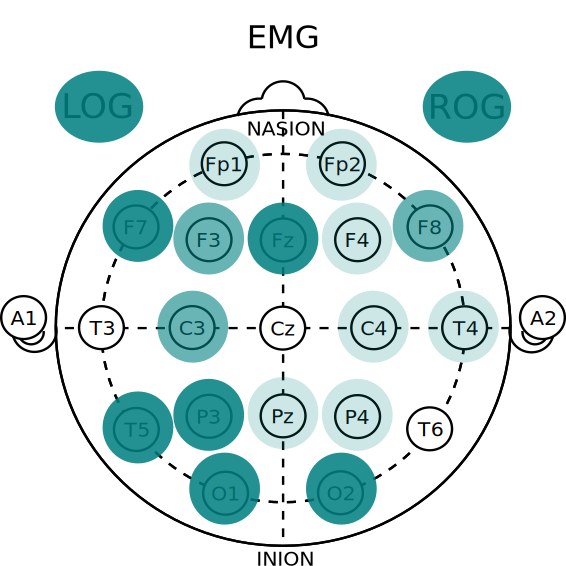
\includegraphics[width=0.15\textwidth]{./img_diagramas/cabecita_GHA.pdf} &
\includegraphics[width=0.15\textwidth]{./img_diagramas/cabecita_MFGR.pdf} \\
VCR & MJH & JAE & GHA & MFGR
\end{tabular}
\\
\begin{tabular}{cccc}
\includegraphics[width=0.15\textwidth]{./img_diagramas/cabecita_CLO.pdf} &
\includegraphics[width=0.15\textwidth]{./img_diagramas/cabecita_RLO.pdf} &
\includegraphics[width=0.15\textwidth]{./img_diagramas/cabecita_RRU.pdf} &
\includegraphics[width=0.15\textwidth]{./img_diagramas/cabecita_JGZ.pdf} \\
CLO & RLO & RRU & JGZ
\end{tabular}
\\
\begin{tabular}{ccc}
\includegraphics[width=0.15\textwidth]{./img_diagramas/cabecita_FGH.pdf} &
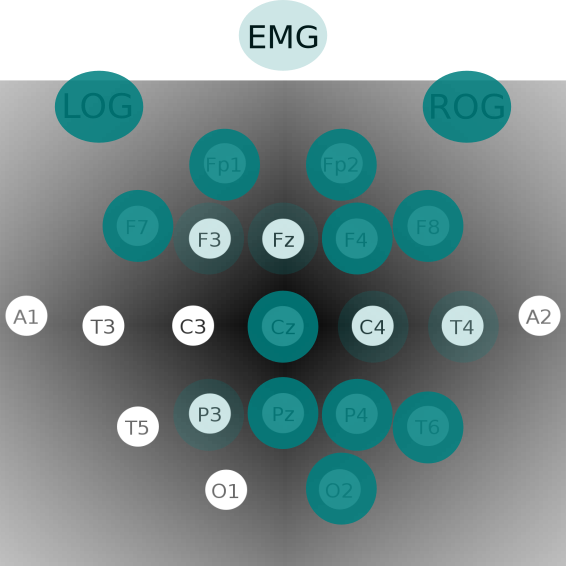
\includegraphics[width=0.15\textwidth]{./img_diagramas/cabecita_MGG.pdf} &
\includegraphics[width=0.15\textwidth]{./img_diagramas/cabecita_EMT.pdf} \\
FGH & MGG & EMT
\end{tabular}
\end{tabular}
\caption{Regiones donde se encontraron diferencias significativas al comparar las proporciones de 
épocas estacionarias durante sueño MOR y NMOR}
\label{cabecitas_munchas}
\end{figure}

Para corroborar la consistencia de las diferencias en LOG y ROG, se repitió la comparación a nivel 
grupal usando la prueba $U$ de  Mann-Whitney\footnote{Implementada en R como \texttt{wilcox.test}}
y se encontraron diferencias significativas ($p<0.05$) para el grupo Nn en los canales C4, F7, FP1, 
FP2, LOG y ROG, mientras que en el grupo Mn sólo se observaron tales diferencias en FP1, LOG y ROG 
(ver figura \ref{comparacion_verde});
las diferencias en la región frontal podrían ser fisiológicamente relevantes, ya que típicamente se 
asocia a la corteza frontal con la toma de decisiones.

El que se encontraran diferencias significativas para el grupo Nn, pero que no se encontraron en el
grupo Mn, sugiere que éstas pueden estar asociadas con el deterioro cognitivo.
Para probar tal hipótesis se comparó grupalmente la proporción de épocas estacionarias, tanto en
sueño MOR como NMOR (ver figura \ref{comparacion_graf}); no se encontraron diferencias
significativas ($p<0.05$).

\begin{figure}
\centering
\includegraphics[width=\linewidth]
{./img_ejemplos/Comparacion_etapas_normal_MOR_vs_NMOR_v2.pdf} \\
\includegraphics[width=\linewidth]
{./img_ejemplos/Comparacion_etapas_pdc_MOR_vs_NMOR_v2.pdf} \\
\caption{Comparación sobre las proporciones de épocas estacionarias durante sueño MOR y NMOR, para 
ambos grupos}
\label{comparacion_verde}
\end{figure}

\begin{figure}
\centering
\includegraphics[width=\linewidth]
{./img_ejemplos/Comparacion_gpos_MOR_v2.pdf} \\
\includegraphics[width=\linewidth]
{./img_ejemplos/Comparacion_gpos_NMOR_v2.pdf}
\caption{Comparación sobre las proporciones de épocas estacionarias entre los grupos Nn y Mn, 
durante sueño MOR y NMOR}
\label{comparacion_graf}
\end{figure}

%%%%%%%%%%%%%%%%%%%%%%%%%%%%%%%%%%%%%%%%%%%%%%%%%%%%%%%%%%%%%%%%%%%%%%%%%%%%%%%%%%%%%%%%%%%%%%%%%%%
%%%%%%%%%%%%%%%%%%%%%%%%%%%%%%%%%%%%%%%%%%%%%%%%%%%%%%%%%%%%%%%%%%%%%%%%%%%%%%%%%%%%%%%%%%%%%%%%%%%

\section{Patrones visuales}

Los resultados anteriores, aparentemente contradictorios, indican que la comparación directa no es 
una herramienta efectiva para entender los cambios que se esperan en la estacionariedad durante
sueño MOR.
Como auxiliar visual, se \textit{graficaron} en el tiempo las épocas
estacionarias indicando por cada canal la porción del registro que se comporta como débilmente 
estacionario, como en la figura \ref{patroncito}.

%\begin{figure}
%\includegraphics[width=\textwidth]
%{./img_ejemplos/MJNNVIGILOS_est.png}
%\caption{Disposición gráfica para los resultados de la prueba PSR en el sujeto MJH. Se han 
%resaltado con color verde las épocas clasificadas como de sueño MOR.}
%\label{ejemplo_graf}
%\end{figure}

Al construir estos gráficos, se hacen visibles \textit{bloques} de épocas con propiedades 
similares; ha parecido conveniente investigar este fenómeno porque su estructura es independiente 
de los métodos planteados. En principio, la aparición de estos bloques es consistente con la
caracterización del sueño por etapas; por ejemplo,
estos bloques aparecen relacionados con la aparición de sueño MOR en todos los 
sujetos del grupo Mn bajo el siguiente patrón:
\begin{itemize}
\item Bloque abundante en épocas estacionarias, visualmente oscuro
\item Bloque abundante en épocas no-estacionarias, visualmente claro
\item Sección que contiene el sueño MOR
\end{itemize}

\begin{figure}
\includegraphics[width=\textwidth]
{./img_ejemplos/zoom_VCR.pdf}
\caption{Patrón propuesto como asociado con el sueño MOR: épocas estacionarias 
(rojo), épocas no-estacionarias (azul), bloque que contiene al sueño MOR}
\label{patroncito}
\end{figure}

Debido a que estos \textit{patrones de estacionariedad} se basan primeramente en propiedades del
espectro de potencias, se graficó el mismo para poder compararlos. Se encontró que, visualmente,
los patrones en la estacionariedad están relacionados con las ondas Beta.

El hecho que estos patrones se encuentren definidos vagamente ha dificultado su análisis, motivo
por el cual su estudio es limitado y se pretende como trabajo futuro.

%%%%%%%%%%%%%%%%%%%%%%%%%%%%%%%%%%%%%%%%%%%%%%%%%%%%%%%%%%%%%%%%%%%%%%%%%%%%%%%%%%%%%%%%%%%%%%%%%%%
%%%%%%%%%%%%%%%%%%%%%%%%%%%%%%%%%%%%%%%%%%%%%%%%%%%%%%%%%%%%%%%%%%%%%%%%%%%%%%%%%%%%%%%%%%%%%%%%%%%
%%%%%%%%%%%%%%%%%%%%%%%%%%%%%%%%%%%%%%%%%%%%%%%%%%%%%%%%%%%%%%%%%%%%%%%%%%%%%%%%%%%%%%%%%%%%%%%%%%%
%%%%%%%%%%%%%%%%%%%%%%%%%%%%%%%%%%%%%%%%%%%%%%%%%%%%%%%%%%%%%%%%%%%%%%%%%%%%%%%%%%%%%%%%%%%%%%%%%%%

\section{Discusión}

Este trabajo parte de la hipótesis de que adultos mayores con PDC presentan en mayor medida 
estacionariedad débil en sus registros de PSG; al comparar sujetos de los grupo Nn (control) y Mn 
(PDC), no se observaron cambios significativos en la porción de tiempo durante la cual el registro 
de PSG se comporta como débilmente estacionario. 
Esto puede interpretarse como que los cambios en la corteza cerebral durante el deterioro 
cognitivo, no provocan que  la señal se vuelva más \textit{simple} en el sentido de 
\textit{volverse} estacionaria.

Comparando grupalmente la cantidad de épocas estacionarias durante MOR y NMOR, se encontró que en 
el grupo Nn había diferencias significativas en sitios de la región frontal y que no eran presentes
en el grupo Mn; para poder establecer una relación con el PDC haría falta un mayor grupo muestral, 
o bien nuevos registros de PSG para los mismos sujetos, o incluso analizar registros de EEG durante 
otro tipo de actividades y confirmar las diferencias encontradas.

Cabe destacar que la evidencia aportada indica que el PSG es un conjunto de señales que se comportan
como no-estacionarias durante la mayor parte del sueño, lo cual confirma el supuesto usual de que 
las señales de origen biológico son por naturaleza no-estacionarias. 

\subsection{Efecto del tamaño de las época}

Como se mencionó anteriormente, el uso de épocas de 30 segundos está motivado por las 
recomendaciones de la AASM para clasificar, de manera estandarizada, las etapas de sueño en
registros de PSG \cite{AASM07}. 
%No se discutirán en este trabajo motivaciones o evidencia para usar esta longitud de época en 
%particular, ni para el caso contrario, sino que se acepta por fines de comparabilidad. 
Debido a un error técnico, en una etapa temprana de este trabajo se usaron épocas de 10 segundos 
para algunos análisis, una inconsistencia que eventualmente fue corregida.
Al efectuar los análisis descritos con otro tamaño de época, se produjeron resultados que distan
bastante de los finales, razón por la cual pareció conveniente investigar más este fenómeno.

En el apéndice X se explica que si disminuye el tamaño de época el test de PSR disminuye su 
potencia, de modo que es más propensa a dar falsos negativos (rechazar la hipótesis de 
estacionariedad cuando debía aceptarse); entonces, en épocas más pequeñas debería haber más épocas 
clasificadas como no-estacionarias.
Sin embargo, al \textit{graficar} la estacionariedad para diferentes tamaños de época (figura
\ref{comp_VCR}) ocurre que es más frecuente el efecto contrario.

\begin{figure}
\centering
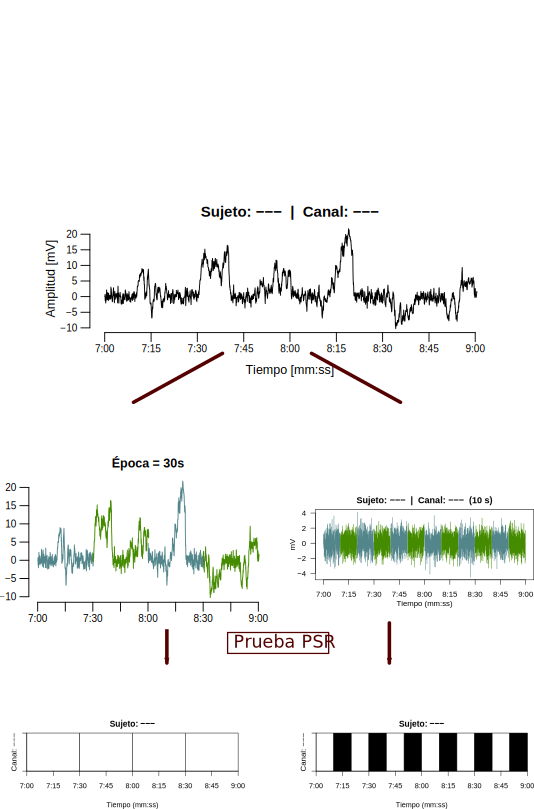
\includegraphics[width=\linewidth]{./img_diagramas/epocas_diferentes_v2.pdf}
\caption{Esquema de cómo se tomaron diferentes tamaños de época para estudiar los registros de 
PSG}
\label{epocas_diferentes}
\end{figure}

Se propone que este efecto puede ser explicado si los registros de PSG son \textbf{localmente
estacionarios}, una propiedad introducida por Dahlhaus \cite{Dahlhaus97} y que consiste en que un
proceso no-estacionario pueda ser aproximado a trozos \textit{ensamblando} procesos estacionarios
definidos para intervalos pequeños de tiempo.
Esta caracterización del EEG ha sido usada anteriormente de manera fructífera pero problemática
[??].

En el contexto particular del presente trabajo, la presencia de estacionariedad local puede ser
explicada fisiológicamente por el contenido heterogéneo de ritmos cerebrales de las etapas de 
sueño; como ejemplo, en la etapa N3 aparecen husos de sueño mezcladas con ritmos Alfa, de modo
que es posible hallar un fragmento de época en sueño N3 con únicamente un tren de ondas Alfa
o un tren de husos de sueño.
Este fenómeno es ilustrado de manera esquemática en la figura \ref{epocas_diferentes}.

\begin{figure}
\centering
\includegraphics[width=0.7\linewidth]
{./img_ejemplos/VCNNS1_comp_est_.png}
\caption{Compilación gráfica de las épocas clasificadas como PE, distribuidas en el tiempo
para cada uno de los canales. El registro corresponde al sujeto VCR, organizando el registro en
épocas de diferente duración}
\label{comp_VCR}
\end{figure}

Entonces, se propone que los registros de PSG se comportan como procesos localmente estacionarios; 
más aún, se propone que esta característica cambia cualitativamente en adultos mayores con PDC,
para los cuales el \textit{nivel de homogeneidad} del PSG es muy similar durante MOR y NMOR.

%%%%%%%%%%%%%%%%%%%%%%%%%%%%%%%%%%%%%%%%%%%%%%%%%%%%%%%%%%%%%%%%%%%%%%%%%%%%%%%%%%%%%%%%%%%%%%%%%%%
%%%%%%%%%%%%%%%%%%%%%%%%%%%%%%%%%%%%%%%%%%%%%%%%%%%%%%%%%%%%%%%%%%%%%%%%%%%%%%%%%%%%%%%%%%%%%%%%%%%

%\subsection{Sobre los sujetos excluidos}
%
%Durante el trabajo se mencionan tres sujetos (FGH, MGG, EMT) cuyos registros de PSG fueron 
%analizados pero que no son considerados estadísticamente; cada uno de ellos fue excluido, por 
%diversos motivos, del trabajo por Vázquez Tagle y colaboradores \cite{VazquezTagle16}, pero 
%dieron su consentimiento informado para el registro de PSG, debido a lo cual analizó el efecto de 
%su inclusión dentro de los análisis.
%Destaca el sujeto FGH, quien padece de parálisis facial, cataratas, y problemas no especificados 
%en hipotiroides y columna; según se reporta, el sujeto no informó de estos últimos 
%padecimientos sino hasta después del registro de PSG, por lo que su exclusión se efectuó a 
%posteriori.
%
%Un vistazo a los registros 'inusuales' de FGH (figura\ref{FGH_psg}, comparar con 
%\ref{ejemplos_mor}) pudiera haber advertido que en el registro no hay actividad cerebral en los 
%canales correspondientes a la región izquierda (aquella con parálisis) sino ruido amplificado 
%del polisomnógrafo.
%Dentro del marco de este trabajo, destacan las proporciones inusuales de épocas PE (cercanas a 1 
%o 0) para este sujeto en los canales F4, F7, F8, FP1, FP2, FZ, tanto en sueño MOR como NMOR; 
%usando la representación gráfica para FGH, es visible una inusual ausencia total de 
%estacionariedad en tales canales (figura \ref{FGH_especial}, comparar con \ref{ejemplo_graf}). 
%Si bien esta metodología no se diseñó para tal fin, aún así se pudo detectar la falta de 
%actividad cerebral.
%
%\begin{figure}
%\centering
%\includegraphics[width=0.95\linewidth]
%{./img_ejemplos/FGH_297_PDG_lucirse_PSG.pdf} 
%\caption{Una época típica del registro PSG para el sujeto FGH durante sueño MOR. Nótense 
%los patrones periódicos en los canales correspondientes a la región frontal, que no 
%corresponden a la actividad cerebral usual.}
%\label{FGH_psg}
%\end{figure}
%
%\begin{figure}
%\centering
%\includegraphics[width=0.95\linewidth]
%{./img_ejemplos/FGHSUE_est.png} 
%\caption{Compilado gráfico para el sujeto FGH; nótese el patrón inusual (completamente 
%blanco o negro) en los canales correspondientes a la región frontal}
%\label{FGH_especial}
%\end{figure}

%%%%%%%%%%%%%%%%%%%%%%%%%%%%%%%%%%%%%%%%%%%%%%%%%%%%%%%%%%%%%%%%%%%%%%%%%%%%%%%%%%%%%%%%%%%%%%%%%%%
%%%%%%%%%%%%%%%%%%%%%%%%%%%%%%%%%%%%%%%%%%%%%%%%%%%%%%%%%%%%%%%%%%%%%%%%%%%%%%%%%%%%%%%%%%%%%%%%%%%

%%%%%%%%%%%%%%%%%%%%%%%%%%%%%%%%%%%%%%%%%%%%%%%%%%%%%%%%%%%%%%%%%%%%%%%%%%%%%%%%%%%%%%%%%%%%%%%%%%%
%%%%%%%%%%%%%%%%%%%%%%%%%%%%%%%%%%%%%%%%%%%%%%%%%%%%%%%%%%%%%%%%%%%%%%%%%%%%%%%%%%%%%%%%%%%%%%%%%%%

\section{Conclusiones}

En registros de PSG para adultos mayores, segmentados en épocas de 30 segundos, la presencia 
proporcional de estacionariedad débil es significativamente diferente ($p<0.05$) durante el sueño 
MOR y NMOR;
Estas diferencia fueron presentes para el grupo Mn en los canales C4, F7, FP1, FP2, LOG, ROG, y 
para el grupo Mn en los canales LOG y ROG.
Estas diferencias pueden explicarse 
(1) en LOG y ROG por las características del sueño MOR y
(2) en los canales C4, F7, FP1, FP2, por tratarse del lóbulo frontal, típicamente asociado con la 
toma de decisiones.

%El análisis de estacionariedad sobre registros de PSG para un adulto mayor con parálisis facial 
%fue capaz de señalar este padecimiento, visto como una ausencia total de épocas estacionarias
%en una región concreta.

Estos resultados sugieren que el método de comparación es sensible a los cambios funcionales del 
cerebro al transitar entre etapas de sueño; tales cambios son menos \textit{visibles} en presencia
de PDC. Esta interpretación propuesta es consistente con \cite{Valeria}.

%En otro ámbito, los patrones visuales descritos, visibles al mostrar gráficamente la 
%distribución de épocas PE, predicen parcialmente con las épocas de sueño MOR clasificadas 
%por un experto (cuando menos en el grupo Control).
%Se propone que la representación gráfica pudiera ser usado como auxiliar en la clasificación 
%de segmentos de registro según la etapa de sueño.

Los datos recabados son evidencia que los registros de PSG en adultos mayores no pueden 
considerarse en general como series de tiempo estacionarias o no-estacionarias, sino que sus 
propiedades estadísticas cambian en el tiempo conforme se transita entre diferentes estados 
fisiológicos; 
%esta característica no puede ser ignoradaal modelar este tipo de señales.
esta característica ha sido considerada anteriormente \cite{Kaiser00}, pero usualmente es ignorada
en base al diseño experimental.

%%%%%%%%%%%%%%%%%%%%%%%%%%%%%%%%%%%%%%%%%%%%%%%%%%%%%%%%%%%%%%%%%%%%%%%%%%%%%%%%%%%%%%%%%%%%%%%%%%%
%%%%%%%%%%%%%%%%%%%%%%%%%%%%%%%%%%%%%%%%%%%%%%%%%%%%%%%%%%%%%%%%%%%%%%%%%%%%%%%%%%%%%%%%%%%%%%%%%%%

\section{Trabajo a futuro}

%Los resultados principales de este trabajo, con vista al trabajo futuro, consiste en las 
%diferencias encontradas entre el sueño MOR y NMOR, así como los patrones visuales asociados con 
%la aparición de sueño MOR; tales características sólo fueron presentes para el grupo 
%Control. Si bien no constituyen propiamente marcadores de deterioro cognitivo, esta metodología
%podría extenderse para identificar tales marcadores.
%Por ejemplo, un marcador conocido \cite{Becerra12} del deterioro cognitivo es el 'enlentecimiento' 
%de la actividad cerebral, entendido como un cambio en la concentración de energía desde ondas 
%rápidas a ondas lentas.
%Para detectar la estacionariedad débil se ha usado prueba de Priestley-Subba Rao, basada en 
%estimadores locales para la función de densidad espectral (FDE); estos mismos estimadores 
%podrían ser usados para corroborar si efectivamente existen diferencias en la FDE para registros 
%de adultos mayores con y sin deterioro cognitivo. 
%
%Finalmente, y como se mencionó anteriormente, los patrones visuales en la representación 
%gráfica pueden tener un uso como características auxiliares para la detección 
%semi-automática de épocas MOR en registros de PSG; en ese sentido, cabe mencionar el caso de 
%los sujetos excluidos del estudio, para los cuales estos patrones parecen no cumplirse. 
%Es en principio posible que la identificabilidad del sueño MOR, a través de estos patrones, 
%pudiera fungir como marcador clínico.

%%%%%%%%%%%%%%%%%%%%%%%%%%%%%%%%%%%%%%%%%%%%%%%%%%%%%%%%%%%%%%%%%%%%%%%%%%%%%%%%%%%%%%%%%%%%%%%%%%%
%%%%%%%%%%%%%%%%%%%%%%%%%%%%%%%%%%%%%%%%%%%%%%%%%%%%%%%%%%%%%%%%%%%%%%%%%%%%%%%%%%%%%%%%%%%%%%%%%%%
%%%%%%%%%%%%%%%%%%%%%%%%%%%%%%%%%%%%%%%%%%%%%%%%%%%%%%%%%%%%%%%%%%%%%%%%%%%%%%%%%%%%%%%%%%%%%%%%%%%
%%%%%%%%%%%%%%%%%%%%%%%%%%%%%%%%%%%%%%%%%%%%%%%%%%%%%%%%%%%%%%%%%%%%%%%%%%%%%%%%%%%%%%%%%%%%%%%%%%%


\appendix

%%%%%%%%%%%%%%%%%%%%%%%%%%%%%%%%%%%%%%%%%%%%%%%%%%%%%%%%%%%%%%%%%%%%%%%%%%%%%%%%%%%%%%%%%%%%%%%%%%%%
%%%%%%%%%%%%%%%%%%%%%%%%%%%%%%%%%%%%%%%%%%%%%%%%%%%%%%%%%%%%%%%%%%%%%%%%%%%%%%%%%%%%%%%%%%%%%%%%%%%
%%%%%%%%%%%%%%%%%%%%%%%%%%%%%%%%%%%%%%%%%%%%%%%%%%%%%%%%%%%%%%%%%%%%%%%%%%%%%%%%%%%%%%%%%%%%%%%%%%%
%%%%%%%%%%%%%%%%%%%%%%%%%%%%%%%%%%%%%%%%%%%%%%%%%%%%%%%%%%%%%%%%%%%%%%%%%%%%%%%%%%%%%%%%%%%%%%%%%%%
\chapter{Detalles}

Se exponen varios de los conceptos expuestos como preeliminares pero con las formalidades
pertinentes; cabe mencionar que todos estos resultados no son originales del presente trabajo,
razón por la cual fueron omitidos anteriormente.
%presentados como preeliminares, incluyendo demostraciones. 
%Esta informaci\'on fue cortada del 
%cuerpo principal del trabajo porque no son resultados originales, y si bien son sumamaente
%importantess e interesantes, se omitieron a favor de los resultados originales generados en el 
%trabajo.

%%%%%%%%%%%%%%%%%%%%%%%%%%%%%%%%%%%%%%%%%%%%%%%%%%%%%%%%%%%%%%%%%%%%%%%%%%%%%%%%%%%%%%%%%%%%%%%%%%%
%%%%%%%%%%%%%%%%%%%%%%%%%%%%%%%%%%%%%%%%%%%%%%%%%%%%%%%%%%%%%%%%%%%%%%%%%%%%%%%%%%%%%%%%%%%%%%%%%%%

\section{Variables aleatorias}

Un primer motivo para esta sección es enfatizar que formalmente una variable aleatoria se concibe 
no como un recuento de eventos sino como una función de medida. Esta segunda 
caracterización es relevante para varios resultados utilizados, por lo que
conviene no omitirla.

Antes de poder definir formalmente las variable aleatoria, debe definirse las medidas.

\begin{defn}[$\boldsymbol{\sigma}$-álgebra]
Sea $U$ un conjunto y $\mathcal{U}$ una colección de subconjuntos de $U$. Se dice que $\mathcal{U}$
es una $\sigma$-álgebra si comple que
\begin{itemize}
\item $U \in \mathcal{U}$
\item $A \in \mathcal{U}$ implica que $A^{C} \in \mathcal{U}$
\item Si $\{ A_n \}_{n\in \mathbb{N}}$ son conjuntos tales que $A_i \in \mathcal{U}$, entonces
$\displaystyle \cup_{n\in \mathbb{N}} A_n \in \mathcal{U}$
\end{itemize}
Donde $A^{C}$ es el complemento $\{ u \in U | u \notin A \} $
\end{defn}

Por simplicidad, en este trabajo sólo se usarán medidas para conjuntos de números reales derivadas 
de la $\sigma$-álgebra de Borel, que es definida como la $\sigma$-álgebra más pequeña que contiene a 
los intervalos abiertos abiertos\footnote{Si una $\sigma$-álgebra contiene a todos los
intervalos abiertos, entonces debe contener a todos los elementos de la $\sigma$-álgebra de Borel}.

\begin{defn}[Medida]
Sea $U$ un conjunto y $\mathcal{U}$ una $\sigma$-álgebra definida en $U$. Se dice que una función
$\mu : \mathcal{U} \rightarrow \R^{*}$ es una medida si cumple que
\begin{itemize}
\item $\mu(\emptyset) = 0$
\item $\mu(A) \geq 0$ para cualquier $A \in \mathcal{U}$
\item Si $\{ A_n \}_{n\in \mathbb{N}}$ son conjuntos disjuntos a pares y tales que 
$A_i \in \mathcal{U}$, entonces 
$\displaystyle \mu\left( \cup_{n\in \mathbb{N}} A_n \right) = \sum_{n\in \mathbb{N}} \mu(A_n)$
\end{itemize}
Donde $\R^{*}$ designa a los 'reales extendidos' $\R \cup \{-\infty,\infty \}$
\end{defn}

\begin{defn}[Medida de probabilidad en $\boldsymbol{\R}$]
Sea $\mathcal{B}$ la sigma álgebra de Borel definida para $\R$, se dice que una función
$P : \mathcal{B} \rightarrow [0.1]$ es una \textbf{medida de probabilidad} si cumple que
\begin{itemize}
\item $P(\emptyset) = 0$
\item $0 \leq P(A) \leq 1$ para cualquier $A \in \mathcal{B}$
\item Si $A, B \in \mathcal{B}$ y $A\cap B = \emptyset$, entonces $P(A \cup B) = P(A) + P(B)$ 
\item $P(\R) = 1$
\end{itemize}
\label{variable_aleatoria}
\end{defn}

%Cabe mencionar que cuando se usa una variable aleatoria para modelar un fenómeno, existe un paso
%intermedio en que los eventos relevantes se asocian con números reales

Una forma de entender mejor una variables aleatoria es a partir de su función de probabilidad
acumulada (FPA), que a su vez caracteriza a la variable: es equivalente referirse
a una variable aleatoria o a su FPA.

\begin{defn}[Función de Probabilidad Acumulada]
Sea 
\begin{equation*}
F_X (x) = P\left( (-\infty,x] \right)
\end{equation*}
\end{defn}

%%%%%%%%%%%%%%%%%%%%%%%%%%%%%%%%%%%%%%%%%%%%%%%%%%%%%%%%%%%%%%%%%%%%%%%%%%%%%%%%%%%%%%%%%%%%%%%%%%%
%%%%%%%%%%%%%%%%%%%%%%%%%%%%%%%%%%%%%%%%%%%%%%%%%%%%%%%%%%%%%%%%%%%%%%%%%%%%%%%%%%%%%%%%%%%%%%%%%%%

\section{Algunas consecuencias de la estacionariedad}

\begin{defn}[Estacionariedad de orden $\boldsymbol{m}$]
Un proceso estoc\'astico $\{ X(t) \}$ se dice estacionario de orden $m$ si, para cualquier conjunto 
de tiempos admisibles $t_1,t_2,\dots,t_n$ y cualquier $\tau \in \R$ se cumple que
\begin{equation*}
\E{ X^{m_1}(t_1)X^{m_2}(t_2)\cdots X^{m_n}(t_n) }
=
\E{ X^{m_1}(t_1+\tau)X^{m_2}(t_2+\tau)\cdots X^{m_n}(t_n+\tau) }
\end{equation*}
Para cualesquiera enteros $m_1,m_2,\dots,m_n$ tales que $m_1+m_2+\dots+m_n \leq m$
\label{est_orden_m}
\end{defn}

Para entender mejor la definici\'on \ref{est_orden_m} y sus limitaciones frente a la 
estacionariedad fuerte, consid\'erense tres procesos: $\{X(t)\}$ fuertemente estacionario, 
$\{Y_1(t)\}$ estacionario de orden 1, y $\{Y_2(t)\}$ estacionario de orden 2. Luego
\begin{itemize}
\item Las medias\footnote{La media de una variable aleatoria $V$ se define como $ \mu_V := \E{V}$} 
$ \mu_{X(t)}$, $ \mu_{Y_1(t)}$ y $ \mu_{Y_2(t)}$ no dependen de $t$

\item Las varianzas\footnote{La varianza de una variable aleatoria $V$ se define como 
$ \Var{V} := \E{\left(V - \mu_V \right)^{2}}$} $ \Var{Y_1(t)}$ y $ \Var{Y_2(t)}$ no dependen de 
$t$, pero no se puede garantizar lo mismo para $\Var{X(t)}$

\item El coeficiente de asimetr\'ia\footnote{El coeficiente de asimetr\'ia para una variable 
aleatoria $V$ se define como 
$\gamma_V = \frac{\E{\left(V-\mu_V\right)^{3}}}{\Var{V}^{\nicefrac{3}{2}}}$}
$ \gamma_{X(t)}$ no depende de $t$, pero no se puede garantizar lo mismo para $ \gamma_{Y_1(t)}$ ni 
para $ \gamma_{Y_2(t)}$
\end{itemize}

Cabe mencionar que hay una relaci\'on de contenci\'on clara en familia de los conjuntos de procesos 
estacionarios de orden finito (si un proceso es estacionario de orden $m$, entonces es estacionario 
de orden $n$ para todo $n \leq m$); es posible definir procesos estacionarios de orden 'infinito' 
seg\'un \ref{est_orden_m}, que intuitivamente ser\'ian fuertemente estacionarios. 
De manera pragm\'atica, en este trabajo no se discuten tales interrogantes, sino que se usar\'a 
\'unicamente la definici\'on correspondiente al caso $m=2$, referida como estacionariedad d\'ebil o 
de orden 2, y repetida en la definici\'on \ref{est_orden_2}.

-----------------

Cabe comentar  sobre la existencia de procesos que son fuertemente estacionarios pero que no son 
estacionarios de ning\'un orden: por ejemplo, un proceso de variables aleatorias independientes con 
distribuci\'on de Cauchy\footnote{Una variable aleatoria tiene distribuci\'on de Cauchy si su 
funci\'on de probabilidad acumulada es de la forma 
$\displaystyle F(x) = \frac{1}{\pi} \int_{-\infty}^{x} \frac{1}{1+y^{2}} dy$}.
Una condici\'on suficiente para que un proceso fuertemente estacionario sea estacionario de orden 
$m$ es que tenga sus primeros $m$ momentos bien definidos.
Con respecto a las se\~nales registradas en el EEG, entendidas como procesos estoc\'asticos, se 
espera que tengan (cuando menos) segundos momentos bien definidos; m\'as adelante se presentan 
argumentos, desde una interpretaci\'on f\'isica, sobre por qu\'e se espera que ocurra lo anterior.



-------------------

Como ejemplos, un proceso ruido blanco (definici\'on \ref{r_blanco}) no es estoc\'asticamente 
continuo, mientras que un proceso de Wiener (definici\'on \ref{r_wiener}) s\'i lo es.

\begin{defn}[Proceso ruido blanco]
Se dice de un proceso estoc\'astico $\{ R(t) \}$ que cumple, para cualesquiera tiempos admisibles
$t$ y $s$, las siguientes propiedades:
\begin{itemize}
\item $\E{R(t)}=0$
\item $\Cov{R(t),R(s)}=0 \Leftrightarrow t=s$ 
\end{itemize}
\label{r_blanco}
\end{defn}

\begin{defn}[Proceso de Wiener]
Se dice de un proceso estoc\'astico $\{ W(t) \}$ que cumple, para cualesquiera tiempos admisibles
$t$ y $s$ (con $s>t$) las siguientes propiedades:
\begin{itemize}
\item $W(0) = 0$ ($W(0)$ es constante)
\item $W(s)-W(t)$ es independiente de $W(u)$, para todo $u<t$ admisible
\item $W(s)-W(t) \sim N(0,\abso{t-s})$  (los incrementos tienen distribuci\'on normal)
\end{itemize}
\label{r_wiener}
\end{defn}

--------------------------

En la definici\'on \ref{fourier_stieltjes}, si $F$ es derivable en todas partes entonces $F\prima$ 
cumple el mismo papel que la integral de Fourier; en cambio, si $k$ es una funci\'on peri\'odica 
entonces $F$ toma una forma escalonada cuyos aumentos coinciden con la serie de Fourier para $k$. 
M\'as a\'un, existen funciones que no son ni peri\'odicas ni absolutamente sumables pero poseen 
una transformada de Fourier-Stieltjes, como $k(x)=\SEN{x}+\SEN{\sqrt{2}x}$, 
$k(x)=\COS{x} + (1+x^{2})^{-1}$.

%\begin{comment}
\begin{thrm}[Descomposici\'on de Lebesgue]
Sea $f:I\rightarrow \R$ una funci\'on de variaci\'on acotada, con $I$ un intervalo. Entonces pueden 
hallarse funciones $f_j, f_c, f_a :I\rightarrow \R$ tales que
\begin{itemize}
\item $f = f_j+ f_c+ f_a$
\item $f_j = \sum_{y \leq x} f(x-0) + f(x+0)$
\item $f_a$ es absolutamente continua\footnote{Para que una funci\'on sea absolutamente continua,
basta que sea de variaci\'on acotada y que mapee conjuntos de medida cero en conjuntos de medida
cero} en $I$
\item $f_c$ es una funci\'on singular\footnote{Una funci\'on es singular si es continua, de 
variaci\'on acotada y no-constante, y se cumple que tiene derivada cero casi en todas partes} en 
$I$
\end{itemize}
Estas funciones son \'unicas excepto por constantes, y en conjunto son llamados la 
\textit{descomposici\'on de Lebesgue} de $f$
\label{Lebesgue_decomp}
\end{thrm}
%\end{comment}

%%%%%%%%%%%%%%%%%%%%%%%%%%%%%%%%%%%%%%%%%%%%%%%%%%%%%%%%%%%%%%%%%%%%%%%%%%%%%%%%%%%%%%%%%%%%%%%%%%%
%%%%%%%%%%%%%%%%%%%%%%%%%%%%%%%%%%%%%%%%%%%%%%%%%%%%%%%%%%%%%%%%%%%%%%%%%%%%%%%%%%%%%%%%%%%%%%%%%%%

\section{Transformada R\'apida de Fourier}

Como se mostró en el texto, la transformada de Fourier es un operador clave para la definición y el
estudio del \textit{dominio de las frecuencias}. Sin embargo, su aplicación a series de tiempo grandes se ve
dificultada porque es un proceso lento: si se toma una serie de tiempo 
$\{s_n\}_{n=0,\dots,N}$ y se calcula su transformada finita de Fourier según su definición
\begin{equation*}
\mathfrak{F}_s(\omega) = \sum_{n=0}^{N} s_n e^{i \omega n}
\end{equation*}
entonces para cada frecuencia $\omega$ se requerirán $N$ multiplicaciones y $N-1$ sumas, siendo que
usualmente se analizan las frecuencias de la forma $\omega_k = \nicefrac{2 \pi k}{N}$ 
con $k = 0, 1, \dots, \nicefrac{N}{2}$.
Usando la notación de Landau (definición \ref{orden}) se deduce que obtener la transformada discreta
de Fourier de una serie de tiempo de longitud $N$, usando este método, 
ocupa un tiempo de orden $\mathcal{O}(N^{2})$.

\begin{defn}[Orden $\mathcal{O}$]
Sean $f, g$ dos funciones en $\R$ con $g(x)\neq 0$ para $x\in \R$. Se dice que $f = \mathcal{O}(g)$,
que $f$ tiene orden $g$, si existe una constante $k\in \R$ tal que
\begin{equation*}
\lim_{x\rightarrow \infty} \frac{f(x)}{g(x)} = k
\end{equation*}
\label{orden}
\end{defn}

El algoritmo presentado por  transformada Rápida de Fourier (TRF) 

%%%%%%%%%%%%%%%%%%%%%%%%%%%%%%%%%%%%%%%%%%%%%%%%%%%%%%%%%%%%%%%%%%%%%%%%%%%%%%%%%%%%%%%%%%%%%%%%%%%
%%%%%%%%%%%%%%%%%%%%%%%%%%%%%%%%%%%%%%%%%%%%%%%%%%%%%%%%%%%%%%%%%%%%%%%%%%%%%%%%%%%%%%%%%%%%%%%%%%%

\section{Efecto del filtro STL}

En el texto se menciona al filtro STL como un algoritmo para eliminar los efectos de tendencias
deterministas sobre los registros, con lo cual se puede argumentar que los registros tienen
valor esperado cero y que admiten una representaci\'on de Wold-Cram\'er. Sin embargo, se omiti\'o
una descripci\'on m\'as adecuada por motivos narrativos.

El algoritmo, introducido por Cleveland y colaboradores en 1990 \cite{Cleveland1990} toma sus siglas
del ingl\'es \textit{Seasonal-Trend decomposition based on Loess} (descomposici\'on en tendencia y
periodicidad basada en loess)

%%%%%%%%%%%%%%%%%%%%%%%%%%%%%%%%%%%%%%%%%%%%%%%%%%%%%%%%%%%%%%%%%%%%%%%%%%%%%%%%%%%%%%%%%%%%%%%%%%%
%%%%%%%%%%%%%%%%%%%%%%%%%%%%%%%%%%%%%%%%%%%%%%%%%%%%%%%%%%%%%%%%%%%%%%%%%%%%%%%%%%%%%%%%%%%%%%%%%%%
%%%%%%%%%%%%%%%%%%%%%%%%%%%%%%%%%%%%%%%%%%%%%%%%%%%%%%%%%%%%%%%%%%%%%%%%%%%%%%%%%%%%%%%%%%%%%%%%%%%
%%%%%%%%%%%%%%%%%%%%%%%%%%%%%%%%%%%%%%%%%%%%%%%%%%%%%%%%%%%%%%%%%%%%%%%%%%%%%%%%%%%%%%%%%%%%%%%%%%%

\input{./texto/anexo_frecuencias.tex}

%%%%%%%%%%%%%%%%%%%%%%%%%%%%%%%%%%%%%%%%%%%%%%%%%%%%%%%%%%%%%%%%%%%%%%%%%%%%%%%%%%%%%%%%%%%%%%%%%%%
%%%%%%%%%%%%%%%%%%%%%%%%%%%%%%%%%%%%%%%%%%%%%%%%%%%%%%%%%%%%%%%%%%%%%%%%%%%%%%%%%%%%%%%%%%%%%%%%%%%
%%%%%%%%%%%%%%%%%%%%%%%%%%%%%%%%%%%%%%%%%%%%%%%%%%%%%%%%%%%%%%%%%%%%%%%%%%%%%%%%%%%%%%%%%%%%%%%%%%%
%%%%%%%%%%%%%%%%%%%%%%%%%%%%%%%%%%%%%%%%%%%%%%%%%%%%%%%%%%%%%%%%%%%%%%%%%%%%%%%%%%%%%%%%%%%%%%%%%%%
\chapter{Detalles}


%%%%%%%%%%%%%%%%%%%%%%%%%%%%%%%%%%%%%%%%%%%%%%%%%%%%%%%%%%%%%%%%%%%%%%%%%%%%%%%%%%%%%%%%%%%%%%%%%%%
%%%%%%%%%%%%%%%%%%%%%%%%%%%%%%%%%%%%%%%%%%%%%%%%%%%%%%%%%%%%%%%%%%%%%%%%%%%%%%%%%%%%%%%%%%%%%%%%%%%

\section{Variable aleatoria}


%%%%%%%%%%%%%%%%%%%%%%%%%%%%%%%%%%%%%%%%%%%%%%%%%%%%%%%%%%%%%%%%%%%%%%%%%%%%%%%%%%%%%%%%%%%%%%%%%%%
%%%%%%%%%%%%%%%%%%%%%%%%%%%%%%%%%%%%%%%%%%%%%%%%%%%%%%%%%%%%%%%%%%%%%%%%%%%%%%%%%%%%%%%%%%%%%%%%%%%

\section{Notas sobre la estacionariedad}

%%%%%%%%%%%%%%%%%%%%%%%%%%%%%%%%%%%%%%%%%%%%%%%%%%%%%%%%%%%%%%%%%%%%%%%%%%%%%%%%%%%%%%%%%%%%%%%%%%%
%%%%%%%%%%%%%%%%%%%%%%%%%%%%%%%%%%%%%%%%%%%%%%%%%%%%%%%%%%%%%%%%%%%%%%%%%%%%%%%%%%%%%%%%%%%%%%%%%%%

\section{Transformada R\'apida de Fourier}


%%%%%%%%%%%%%%%%%%%%%%%%%%%%%%%%%%%%%%%%%%%%%%%%%%%%%%%%%%%%%%%%%%%%%%%%%%%%%%%%%%%%%%%%%%%%%%%%%%%
%%%%%%%%%%%%%%%%%%%%%%%%%%%%%%%%%%%%%%%%%%%%%%%%%%%%%%%%%%%%%%%%%%%%%%%%%%%%%%%%%%%%%%%%%%%%%%%%%%%

%\section{Efecto del filtro STL}

%%%%%%%%%%%%%%%%%%%%%%%%%%%%%%%%%%%%%%%%%%%%%%%%%%%%%%%%%%%%%%%%%%%%%%%%%%%%%%%%%%%%%%%%%%%%%%%%%%%
%%%%%%%%%%%%%%%%%%%%%%%%%%%%%%%%%%%%%%%%%%%%%%%%%%%%%%%%%%%%%%%%%%%%%%%%%%%%%%%%%%%%%%%%%%%%%%%%%%%
%%%%%%%%%%%%%%%%%%%%%%%%%%%%%%%%%%%%%%%%%%%%%%%%%%%%%%%%%%%%%%%%%%%%%%%%%%%%%%%%%%%%%%%%%%%%%%%%%%%
%%%%%%%%%%%%%%%%%%%%%%%%%%%%%%%%%%%%%%%%%%%%%%%%%%%%%%%%%%%%%%%%%%%%%%%%%%%%%%%%%%%%%%%%%%%%%%%%%%%

%%%%%%%%%%%%%%%%%%%%%%%%%%%%%%%%%%%%%%%%%%%%%%%%%%%%%%%%%%%%%%%%%%%%%%%%%%%%%%%%%%%%%%%%%%%%%%%%%%%
%%%%%%%%%%%%%%%%%%%%%%%%%%%%%%%%%%%%%%%%%%%%%%%%%%%%%%%%%%%%%%%%%%%%%%%%%%%%%%%%%%%%%%%%%%%%%%%%%%%
%%%%%%%%%%%%%%%%%%%%%%%%%%%%%%%%%%%%%%%%%%%%%%%%%%%%%%%%%%%%%%%%%%%%%%%%%%%%%%%%%%%%%%%%%%%%%%%%%%%
%%%%%%%%%%%%%%%%%%%%%%%%%%%%%%%%%%%%%%%%%%%%%%%%%%%%%%%%%%%%%%%%%%%%%%%%%%%%%%%%%%%%%%%%%%%%%%%%%%%

\chapter{Espectro evolutivo}

%%%%%%%%%%%%%%%%%%%%%%%%%%%%%%%%%%%%%%%%%%%%%%%%%%%%%%%%%%%%%%%%%%%%%%%%%%%%%%%%%%%%%%%%%%%%%%%%%%%

\section{Espectro evolutivo}

%%%%%%%%%%%%%%%%%%%%%%%%%%%%%%%%%%%%%%%%%%%%%%%%%%%%%%%%%%%%%%%%%%%%%%%%%%%%%%%%%%%%%%%%%%%%%%%%%%%

\section{Estimación del espectro evolutivo}

Una vez definido el espectro evolutivo para procesos no-estacionarios con varianza finita, cabe 
preguntarse sobre le estimación de esta cantidad a partir de una realización del proceso usando, 
por ejemplo, periodogramas modificados; tal pregunta no tiene, en general, una respuesta 
satisfactoria.
Es por ello que se define una colección, más restringida, de procesos no-estacionarios cuyo 
espectro evolutivo pueda ser estimado efectivamente usando la técnica de ventanas.

Considerando un proceso no-estacionario \xt que admite una representación de la forma 
$X(t) = \intR A(t,\omega) e^{i \omega t} dZ(\omega)$, entonces el espectro evolutivo queda definido 
como
\begin{equation}
dF_t(\omega) = \abso{A(t,\omega)}^{2} d\mu(\omega)
\label{esp_evolutivo}
\end{equation}

Antes de poder usar la proposición \ref{pseudo_d} para estimar $F_t$ (con respecto a $t$) usando 
una ventana espectral, hay que medir la dispersión de $F_t$ en el tiempo; más aún, hay que pedir 
que esa dispersión sea finita.
Con vista a la ecuación \ref{esp_evolutivo}, se puede usar la conexión entre $F$ y $A$ para 
establecer condiciones respecto a la segunda; se define entonces a $H_\omega$, la transformada de
Fourier de $A$ en el tiempo
\begin{equation}
A(t,\omega) = \intR e^{i t \theta} dH_\omega(\theta)
\end{equation}

Un motivo muy fuerte para definir un objeto tan rebuscado es que (...)

Posteriormente se define a $B_{\mathbf{F}}$, el ancho de banda para $H_\omega$ con respecto a la 
familia de funciones $\mathbf{F}$, como
%
\begin{equation}
B_{\mathbf{F}}(\omega) = \intR \abso{\theta} \abso{dH_\omega(\theta)}
\end{equation}

Se dice que el proceso es semi-estacionario con respecto a $\mathbf{F}$ si 
$\sup_\omega B_{\mathbf{F}} < \infty$. El proceso se dice simplemente \textbf{semi-estacionario} 
si esta cantidad es acotada para cualquier familia de funciones admisibles 
$\mathbf{F} \in \mathbf{C}$; entonces se puede definir la constante $B_X$, el \textit{ancho de 
banda característico de} \xt, como

\begin{equation}
B_X = \sup_{\mathbf{F}\in \mathbf{C}} \left[ \sup_\omega B_{\mathbf{F}}(\omega) \right]^{-1}
\end{equation}

Muy vagamente, $B_X$ indica el tiempo máximo en el cual el proceso, representado en la forma
\ref{esp_evolutivo}, (...)

Una vez definida la cantidad $B_X$, y habiendo supuesto que no es 0, es demostrado en 
\cite{Priestley65} que el estimador $U$ definido como en ... satisface que
%
\begin{equation}
\E{\abso{U(t,\omega)}^{2}} = \intR \abso{\Gamma(\omega)}^{2} f(t,\omega+\omega_0) d\omega
+ \orden\left( \nicefrac{B_g}{B_X} \right)
\end{equation}

De esta última expresión es evidente que el estimador es mejor conforme 
\begin{itemize}
\item  $B_X$, el tiempo máximo para el cual el proceso es \textit{básicamente estacionario}, es 
mayor
\item $B_g$, la dispersión en el tiempo para la ventana $g$, es menor
\end{itemize}

---

Entonces se ha probado en \cite{Priestley66,Priestley69} que bajo ciertas
condiciones p

\section{Estimador de doble ventana}

Respecto a la estimación del espectro local se usa el \textbf{estimador de doble ventana}, 
técnica introducida por Priestley \cite{Priestley69} y que requiere dos funciones, $w_\tau$ y 
$g$, que funcionan como ventana de retrasos y como filtro lineal, respectivamente.
%
En cuando a $g$, se define a $\Gamma(u) = \intR g(u) e^{i u \omega} du$ y se les pide que
\begin{equation*}
2\pi \int_{-\infty}^{\infty} \lvert g(u) \lvert^{2} du 
= 
\int_{-\infty}^{\infty} \lvert \Gamma(\omega) \lvert^{2} d\omega
= 1
\end{equation*}

Cabe mencionar que las ventanas espectrales mostradas en la tabla \ref{ventanas} bien 
pueden cumplir las propiedades requeridas para ser filtros.
Posteriormente se define el estimador $U$ con el objetivo de asignar pesos en el tiempo para estimar
a la FDE
% en el tiempo dado; más aún, $U$ sirve 
%como una aproximación de la representación de Wold-Cramér para 
%el proceso.
\begin{equation*}
U(t,\omega) = \int_{t-T}^{t} g(u) X({t-u}) e^{i \omega (t-u)} du
\end{equation*}

Bajo el entendido que la función $\Gamma$ converge a una función tipo \dirac, puede 
considerarse que 
$\E{\abso{U(t,\omega)}^{2}} \approx f_t(\omega)$; sin embargo, se demuestra en \cite{Priestley66} 
que $\Var{\abso{U(t,\omega)}^{2}} \nrightarrow 0$.
%
Debido a ello se usa una segunda función tipo ventana,
%, para 'suavizar' el estimador y hacerlo consistente (
de forma similar al periodograma.
Se considera la función $W_\tau$, ventana de retrasos, y su respectiva ventana espectral 
$w_\tau$; deben satisfacer las siguientes propiedades:
\begin{itemize}
\item $w_{\tau}(t) \geq 0$ para cualesquiera $t$, $\tau$
\item $w_{\tau}(t) \rightarrow 0$ cuando $\lvert t \lvert \rightarrow \infty$, para todo $\tau$
\item $\displaystyle \int_{-\infty}^{\infty} w_{\tau}(t) dt = 1$ para todo $\tau$
\item $\displaystyle \int_{-\infty}^{\infty} \left( w_{\tau}(t) \right)^{2} dt < \infty$ para todo $\tau$
\item $\exists C$ tal que  
$\displaystyle \lim_{\tau\rightarrow\infty} \tau \int_{-\infty}^{t} \abso{ W_{\tau}(\lambda) }^{2} d\lambda = C$
\end{itemize}

%Por ejemplo, la ventana de Daniell satisface estas propiedades; para ello, conviene calcular que
%$\lim_{\tau\rightarrow\infty} \tau \int_{t-T}^{t} \lvert W_{\tau}(\lambda) \lvert^{2} d\lambda = 2\pi$;
%más aún, 
Cabe mencionar que todas las ventanas mostradas en \ref{ventanas} satisfacen las propiedades 
anteriores.
Finalmente, se define el estimador $\est{f}$ para las FDE normalizada, $f_t$, como
\begin{equation*}
\widehat{f}(t,\omega) = \int_{t-T}^{t} w_{T'}(u) \lvert U(t-u,\omega) \lvert^{2} du
\label{estimador_doble_ventana}
\end{equation*}

Fue demostrado por Priestley \cite{Priestley65} que los estimadores de doble ventana son 
asintóticamente insesgados y consistentes, y propone las siguientes aproximaciones:
%conviene exhibir las siguientes expresiones aproximadas propuestas en aquél trabajo
\begin{itemize}
\item $\displaystyle
\E{\est{f}(t,\omega)} \approx 
\intR \widetilde{f}(t,\omega+\theta) \abso{\Gamma(\theta)}^{2} d\theta$
\item $\displaystyle
\Var{\est{f}(t,\omega)} \approx \frac{C}{\tau} \left( \overline{f}^{2}(\omega) \right)
\intR \abso{\Gamma(\theta)}^{4} d\theta $
\end{itemize}

donde las funciones $\widetilde{f}$ y $\overline{f}$ son versiones 'suavizadas' de la FDE 
normalizada, $f$, y están definidas de la siguiente manera
\begin{equation*}
\widetilde{f}(t,\omega+\theta) = 
\intR W_{\tau}(u) f(t-u,\omega+\theta) du
\end{equation*}
\begin{equation*}
\overline{f}^{2} (t,\omega) =
\frac{\intR f^{2}\left(t-u,W_{\tau}^{2}(u)\right) du}
{\intR \left( W_{\tau}(u) \right)^{2} du}
\end{equation*}

Como $W_{\tau}$ funciona como ventana espectral, converge a una 
función tipo \dirac; luego $\widetilde{f}$ es aproximadamente la convolución 
$\widetilde{f}(t,\omega+\theta) \approx \delta_t \ast f(\bullet,\omega+\theta)$. 
Una aproximación muy similar 
puede hacerse respecto al segundo término, de modo que $\widetilde{f}\approx f$ y 
$\overline{f}^{2}\approx f^{2}$.
Tales aproximaciones serán mejores en tanto las ventanas $w_{\tau}$ y $W_{\tau}$ sean más 
cercanas a funciones tipo \dirac.
%; más aún, una condición adecuada es que estas funciones 
%tengan una forma 'más delgada' que el espacio entre los tiempos y frecuencias donde se estimará 
%$f$.
Dicho esto, se pueden hacer las siguientes aproximaciones, un poco más arriesgadas:
\begin{itemize}
\item $\displaystyle \E{\est{f}(t,\omega)} \approx f(t,\omega)$
\item $\displaystyle \Var{\est{f}(t,\omega)} \approx 
\frac{C}{\tau} f^{2}(t,\omega) \intR \abso{\Gamma (\theta)}^{4} d\theta$
\end{itemize}

%%%%%%%%%%%%%%%%%%%%%%%%%%%%%%%%%%%%%%%%%%%%%%%%%%%%%%%%%%%%%%%%%%%%%%%%%%%%%%%%%%%%%%%%%%%%%%%%%%%
%%%%%%%%%%%%%%%%%%%%%%%%%%%%%%%%%%%%%%%%%%%%%%%%%%%%%%%%%%%%%%%%%%%%%%%%%%%%%%%%%%%%%%%%%%%%%%%%%%%

%\section{Efecto del filtro STL}

%%%%%%%%%%%%%%%%%%%%%%%%%%%%%%%%%%%%%%%%%%%%%%%%%%%%%%%%%%%%%%%%%%%%%%%%%%%%%%%%%%%%%%%%%%%%%%%%%%%
%%%%%%%%%%%%%%%%%%%%%%%%%%%%%%%%%%%%%%%%%%%%%%%%%%%%%%%%%%%%%%%%%%%%%%%%%%%%%%%%%%%%%%%%%%%%%%%%%%%
%%%%%%%%%%%%%%%%%%%%%%%%%%%%%%%%%%%%%%%%%%%%%%%%%%%%%%%%%%%%%%%%%%%%%%%%%%%%%%%%%%%%%%%%%%%%%%%%%%%
%%%%%%%%%%%%%%%%%%%%%%%%%%%%%%%%%%%%%%%%%%%%%%%%%%%%%%%%%%%%%%%%%%%%%%%%%%%%%%%%%%%%%%%%%%%%%%%%%%%

%\input{./texto/anexo_fisio.tex}

%\input{./texto/eeg.tex}

%\input{./texto/tablas_graficos.tex}
%%%%%%%%%%%%%%%%%%%%%%%%%%%%%%%%%%%%%%%%%%%%%%%%%%%%%%%%%%%%%%%%%%%%%%%%%%%%%%%%%%%%%%%%%%%%%%%%%%%
%%%%%%%%%%%%%%%%%%%%%%%%%%%%%%%%%%%%%%%%%%%%%%%%%%%%%%%%%%%%%%%%%%%%%%%%%%%%%%%%%%%%%%%%%%%%%%%%%%%
%%%%%%%%%%%%%%%%%%%%%%%%%%%%%%%%%%%%%%%%%%%%%%%%%%%%%%%%%%%%%%%%%%%%%%%%%%%%%%%%%%%%%%%%%%%%%%%%%%%
%%%%%%%%%%%%%%%%%%%%%%%%%%%%%%%%%%%%%%%%%%%%%%%%%%%%%%%%%%%%%%%%%%%%%%%%%%%%%%%%%%%%%%%%%%%%%%%%%%%

\chapter{Compilados gráficos}

En este apéndice se muestran los compilados gráficos mencionados en la parte de resultados,
y que representan la
distribución temporal y pseudo-espacial de las ocurrencia de épocas PSG dentro de los registros 
para cada paciente. 

Primeramente se presentan los compilados gráficos en los que se ha destacado el sueño MOR;
posteriormente se presentan los mismos gráficos resaltando los patrones visuales
propuestos, que parecen estar relacionados con la aparición de sueño MOR.


% parche de relleno
\begin{figure}
\centering
\includegraphics[width=.9\linewidth]{./img_resultados/cabeza_VCR.pdf}
%\caption{Porcentajes de épocas estacionarias, VCR (VCNNS1)}
\end{figure}

%%%%%%%%%%%%%%%%%%%%%%%%%%%%%%%%%%%%%%%%%%%%%%%%%%%%%%%%%%%%%%%%%%%%%%%%%%%%%%%%%%%%%%%%%%%%%%%%%%%
%%%%%%%%%%%%%%%%%%%%%%%%%%%%%%%%%%%%%%%%%%%%%%%%%%%%%%%%%%%%%%%%%%%%%%%%%%%%%%%%%%%%%%%%%%%%%%%%%%%

\begin{figure}
\centering
\includegraphics[width=0.9\linewidth]
{./img_ejemplos/VCNNS1_comp_est_.png} 
\end{figure}

\begin{figure}
\centering
\includegraphics[width=0.9\linewidth]
{./img_resultados/VCNNS1_espectral_total.png} 
\end{figure}

\begin{figure}
\centering
\includegraphics[width=0.9\linewidth]
{./img_resultados/VCNNS1_combinado_.png} 
\end{figure}

\begin{figure}
\centering
\includegraphics[width=.9\linewidth]{./img_resultados/cabeza_VCR.pdf}
%\caption{Porcentajes de épocas estacionarias, VCR (VCNNS1)}
\end{figure}

%%%%%%%%%%%%%%%%%%%%%%%%%%%%%%%%%%%%%%%%%%%%%%%%%

\begin{figure}
\centering
\includegraphics[width=0.9\linewidth]
{./img_ejemplos/MJNNVIGILOS_comp_est_.png} 
\end{figure}

\begin{figure}
\centering
\includegraphics[width=0.9\linewidth]
{./img_resultados/MJNNVIGILOS_espectral_total.png} 
\end{figure}

\begin{figure}
\centering
\includegraphics[width=0.9\linewidth]
{./img_resultados/MJNNVIGILOS_combinado_.png} 
\end{figure}

\begin{figure}
\centering
\includegraphics[width=.9\linewidth]{./img_resultados/cabeza_MJH.pdf}
%\caption{Porcentajes de épocas estacionarias, MJH (MJNNVIGILOS)}
\end{figure}

%%%%%%%%%%%%%%%%%%%%%%%%%%%%%%%%%%%%%%%%%%%%%%%%%

\begin{figure}
\centering
\includegraphics[width=0.9\linewidth]
{./img_ejemplos/JANASUE_comp_est_.png} 
\end{figure}
\begin{figure}
\centering
\includegraphics[width=0.9\linewidth]
{./img_resultados/JANASUE_espectral_total.png} 
\end{figure}
\begin{figure}
\centering
\includegraphics[width=0.9\linewidth]
{./img_resultados/JANASUE_combinado_.png} 
\end{figure}

\begin{figure}
\centering
\includegraphics[width=.9\linewidth]{./img_resultados/cabeza_JAE.pdf}
%\caption{Porcentajes de épocas estacionarias, JAE (JANASUE)}
\end{figure}

%%%%%%%%%%%%%%%%%%%%%%%%%%%%%%%%%%%%%%%%%%%%%%%%%

\begin{figure}
\centering
\includegraphics[width=0.9\linewidth]
{./img_ejemplos/GH24031950SUENO_comp_est_.png} 
\end{figure}
\begin{figure}
\centering
\includegraphics[width=0.9\linewidth]
{./img_resultados/GH24031950SUENO_espectral_total.png} 
\end{figure}
\begin{figure}
\centering
\includegraphics[width=0.9\linewidth]
{./img_resultados/GH24031950SUENO_combinado_.png} 
\end{figure}

\begin{figure}
\centering
\includegraphics[width=.9\linewidth]{./img_resultados/cabeza_GHA.pdf}
%\caption{Porcentajes de épocas estacionarias, GHA (GH24031950SUEÑO)}
\end{figure}

%%%%%%%%%%%%%%%%%%%%%%%%%%%%%%%%%%%%%%%%%%%%%%%%%

\begin{figure}
\centering
\includegraphics[width=0.9\linewidth]
{./img_ejemplos/GURM251148SUE_comp_est_.png} 
\end{figure}
\begin{figure}
\centering
\includegraphics[width=0.9\linewidth]
{./img_ejemplos/GURM251148SUE_comp_est_.png} 
\end{figure}
\begin{figure}
\centering
\includegraphics[width=0.9\linewidth]
{./img_ejemplos/GURM251148SUE_comp_est_.png} 
\end{figure}

\begin{figure}
\centering
\includegraphics[width=.9\linewidth]{./img_resultados/cabeza_MFGR.pdf}
%\caption{Porcentajes de épocas estacionarias MFGR (GURM251148SUE)}
\end{figure}

%%%%%%%%%%%%%%%%%%%%%%%%%%%%%%%%%%%%%
%%%%%%%%%%%%%%%%%%%%%%%%%%%%%%%%%%%%%
%%%%%%%%%%%%%%%%%%%%%%%%%%%%%%%%%%%%%

\begin{figure}
\centering
\includegraphics[width=0.9\linewidth]
{./img_ejemplos/CLMN10SUE_comp_est_.png} 
\end{figure}

\begin{figure}
\centering
\includegraphics[width=0.9\linewidth]
{./img_resultados/CLMN10SUE_espectral_total.png} 
\end{figure}

\begin{figure}
\centering
\includegraphics[width=0.9\linewidth]
{./img_resultados/CLMN10SUE_combinado_.png} 
\end{figure}

\begin{figure}
\centering
\includegraphics[width=.9\linewidth]{./img_resultados/cabeza_CLO.pdf}
%\caption{Porcentajes de épocas estacionarias, CLO (CLMN10SUE)}
\end{figure}

%%%%%%%%%%%%%%%%%%%%%%%%%%%%%%%%%%%%%

\begin{figure}
\centering
\includegraphics[width=0.9\linewidth]
{./img_ejemplos/RLMN10SUE_comp_est_.png} 
\end{figure}
\begin{figure}
\centering
\includegraphics[width=0.9\linewidth]
{./img_ejemplos/RLMN10SUE_comp_est_.png} 
\end{figure}
\begin{figure}
\centering
\includegraphics[width=0.9\linewidth]
{./img_ejemplos/RLMN10SUE_comp_est_.png} 
\end{figure}

\begin{figure}
\centering
\includegraphics[width=.9\linewidth]{./img_resultados/cabeza_RLO.pdf}
%\caption{Porcentajes de épocas estacionarias, RLO (RLMN10SUE)}
\end{figure}

%%%%%%%%%%%%%%%%%%%%%%%%%%%%%%%%%%%%%

\begin{figure}
\centering
\includegraphics[width=0.9\linewidth]
{./img_ejemplos/RRMNS_comp_est_.png} 
\end{figure}

\begin{figure}
\centering
\includegraphics[width=0.9\linewidth]
{./img_resultados/RRMNS_espectral_total.png} 
\end{figure}

\begin{figure}
\centering
\includegraphics[width=0.9\linewidth]
{./img_resultados/RRMNS_combinado_.png} 
\end{figure}

\begin{figure}
\centering
\includegraphics[width=.9\linewidth]{./img_resultados/cabeza_RRU.pdf}
%\caption{Porcentajes de épocas estacionarias, RRU (RRMNS)}
\end{figure}

%%%%%%%%%%%%%%%%%%%%%%%%%%%%%%%%%%%%%

\begin{figure}
\centering
\includegraphics[width=0.9\linewidth]
{./img_ejemplos/JGMN6SUE_comp_est_.png} 
\end{figure}

\begin{figure}
\centering
\includegraphics[width=0.9\linewidth]
{./img_resultados/JGMN6SUE_espectral_total.png} 
\end{figure}

\begin{figure}
\centering
\includegraphics[width=0.9\linewidth]
{./img_resultados/JGMN6SUE_combinado_.png} 
\end{figure}

\begin{figure}
\centering
\includegraphics[width=.9\linewidth]{./img_resultados/cabeza_JGZ.pdf}
%\caption{Porcentajes de épocas estacionarias, JGZ (JGMN6SUE)}
\end{figure}

%%%%%%%%%%%%%%%%%%%%%%%%%%%%%%%%%%%%%
%%%%%%%%%%%%%%%%%%%%%%%%%%%%%%%%%%%%%
%%%%%%%%%%%%%%%%%%%%%%%%%%%%%%%%%%%%%

\begin{figure}
\centering
\includegraphics[width=0.9\linewidth]
{./img_ejemplos/FGHSUE_comp_est_.png} 
\end{figure}
\begin{figure}
\centering
\includegraphics[width=0.9\linewidth]
{./img_resultados/FGHSUE_espectral_total.png} 
\end{figure}
\begin{figure}
\centering
\includegraphics[width=0.9\linewidth]
{./img_resultados/FGHSUE_combinado_.png} 
\end{figure}

\begin{figure}
\centering
\includegraphics[width=.9\linewidth]{./img_resultados/cabeza_FGH.pdf}
%\caption{Porcentajes de épocas estacionarias, FGH (FGHSUE)}
\end{figure}

%%%%%%%%%%%%%%%%%%%%%%%%%%%%%%%%%%%%%

\begin{figure}
\centering
\includegraphics[width=0.9\linewidth]
{./img_ejemplos/MGNA5SUE_comp_est_.png} 
\end{figure}
\begin{figure}
\centering
\includegraphics[width=0.9\linewidth]
{./img_ejemplos/MGNA5SUE_comp_est_.png} 
\end{figure}
\begin{figure}
\centering
\includegraphics[width=0.9\linewidth]
{./img_ejemplos/MGNA5SUE_comp_est_.png} 
\end{figure}

\begin{figure}
\centering
\includegraphics[width=.9\linewidth]{./img_resultados/cabeza_MGG.pdf}
%\caption{Porcentajes de épocas estacionarias, MGG (MGNA5SUE)}
\end{figure}

%%%%%%%%%%%%%%%%%%%%%%%%%%%%%%%%%%%%%

\begin{figure}
\centering
\includegraphics[width=0.9\linewidth]
{./img_ejemplos/EMNNS_comp_est_.png} 
\end{figure}
\begin{figure}
\centering
\includegraphics[width=0.9\linewidth]
{./img_ejemplos/EMNNS_comp_est_.png} 
\end{figure}
\begin{figure}
\centering
\includegraphics[width=0.9\linewidth]
{./img_ejemplos/EMNNS_comp_est_.png} 
\end{figure}

\begin{figure}
\centering
\includegraphics[width=.9\linewidth]{./img_resultados/cabeza_EMT.pdf}
%\caption{Porcentajes de épocas estacionarias EMT (EMNNS)}
\end{figure}

%%%%%%%%%%%%%%%%%%%%%%%%%%%%%%%%%%%%%

%\begin{figure}
%\bordes{1.5}
%\begin{tabular}{l}
%\Large{{Patrones visuales}}\\
%\begin{tabular}{c}
%\includegraphics[width=0.45\textwidth]
%{./img_ejemplos/zoom_VCR.pdf}
%\includegraphics[width=0.45\textwidth]
%{./img_ejemplos/zoom_MJH.pdf}
%\\
%\includegraphics[width=0.45\textwidth]
%{./img_ejemplos/zoom_JAE.pdf}
%\includegraphics[width=0.45\textwidth]
%{./img_ejemplos/zoom_GHA.pdf}
%\\
%\includegraphics[width=0.45\textwidth]
%{./img_ejemplos/zoom_MFGR.pdf}
%\end{tabular}
%\end{tabular}
%\end{figure}

%%%%%%%%%%%%%%%%%%%%%%%%%%%%%%%%%%%%%%%%%%%%%%%%%%%%%%%%%%%%%%%%%%%%%%%%%%%%%%%%%%%%%%%%%%%%%%%%%%%
%%%%%%%%%%%%%%%%%%%%%%%%%%%%%%%%%%%%%%%%%%%%%%%%%%%%%%%%%%%%%%%%%%%%%%%%%%%%%%%%%%%%%%%%%%%%%%%%%%%
%%%%%%%%%%%%%%%%%%%%%%%%%%%%%%%%%%%%%%%%%%%%%%%%%%%%%%%%%%%%%%%%%%%%%%%%%%%%%%%%%%%%%%%%%%%%%%%%%%%
%%%%%%%%%%%%%%%%%%%%%%%%%%%%%%%%%%%%%%%%%%%%%%%%%%%%%%%%%%%%%%%%%%%%%%%%%%%%%%%%%%%%%%%%%%%%%%%%%%%


%%%%%%%%%%%%%%%%%%%%%%%%%%%%%%%%%%%%%%%%%%%%%%%%%%%%%%%%%%%%%%%%%%%%%%%%%%%%%%%%%%%%%%%%%%%%%%%%%%%
%%%%%%%%%%%%%%%%%%%%%%%%%%%%%%%%%%%%%%%%%%%%%%%%%%%%%%%%%%%%%%%%%%%%%%%%%%%%%%%%%%%%%%%%%%%%%%%%%%%

{%\small
%\bibliographystyle{abbrv_esp}
%\bibliographystyle{abbrv}
\bibliographystyle{bababbrv}
\bibliography{referencias_estacionariedad,referencias_fisiologia,referencias_otros,referencias_mixto}{}
%\bibliographystyle{apalike-es}
}

%%%%%%%%%%%%%%%%%%%%%%%%%%%%%%%%%%%%%%%%%%%%%%%%%%%%%%%%%%%%%%%%%%%%%%%%%%%%%%%%%%%%%%%%%%%%%%%%%%%
%%%%%%%%%%%%%%%%%%%%%%%%%%%%%%%%%%%%%%%%%%%%%%%%%%%%%%%%%%%%%%%%%%%%%%%%%%%%%%%%%%%%%%%%%%%%%%%%%%%

\end{document}

%%%%%%%%%%%%%%%%%%%%%%%%%%%%%%%%%%%%%%%%%%%%%%%%%%%%%%%%%%%%%%%%%%%%%%%%%%%%%%%%%%%%%%%%%%%%%%%%%%%
%%%%%%%%%%%%%%%%%%%%%%%%%%%%%%%%%%%%%%%%%%%%%%%%%%%%%%%%%%%%%%%%%%%%%%%%%%%%%%%%%%%%%%%%%%%%%%%%%%%
%%%%%%%%%%%%%%%%%%%%%%%%%%%%%%%%%%%%%%%%%%%%%%%%%%%%%%%%%%%%%%%%%%%%%%%%%%%%%%%%%%%%%%%%%%%%%%%%%%%
%%%%%%%%%%%%%%%%%%%%%%%%%%%%%%%%%%%%%%%%%%%%%%%%%%%%%%%%%%%%%%%%%%%%%%%%%%%%%%%%%%%%%%%%%%%%%%%%%%%